\documentclass[oneside]{hcmus-report}
\usepackage{codespace}

% Encodings
\usepackage{gensymb,textcomp}

% Better tables
% Wide tables go to https://tex.stackexchange.com/q/332902

\usepackage{array,longtable,multicol,multirow,siunitx,tabularx}

% Better enum
\usepackage{enumitem}

% Graphics
\usepackage{caption,float}

% Add options for figures, like max width, framing, etc.
\usepackage[export]{adjustbox}

\captionsetup{hypcap=false}

% References
% Use \Cref{} instead of \ref{}
\usepackage[nameinlink]{cleveref}

% FOR DEMONSTRATION PURPOSES, REMOVE IN PRODUCTION
\usepackage{mwe}
\usepackage{graphicx}  
\usepackage{float}     
\usepackage{subcaption}

\usepackage{xurl}
\usepackage{hyperref}
\usepackage{longtable}
\usepackage{amsmath, amssymb}
\usepackage{array}
\usepackage{ltablex}
\keepXColumns

\usepackage{xcolor}
\usepackage{colortbl}

% Configurations
\coursename{Nhập môn học máy}
\reporttype{BÁO CÁO ĐỒ ÁN CUỐI KỲ}
\title{BÁO CÁO DỮ LIỆU}
\advisor{& TS. Bùi Tiến Lên &}
\stuname{%
  & 23120195 & Lê Hà Thanh Chương \\
  & 23120197 & Trà Văn Sỹ \\
  & 23120199 & Huỳnh Đức Thịnh \\
  & 23120257 & Bùi Trung Hiếu \\
  & 23120330 & Lê Công Phúc \\
}

% Set depth of numbering for counters
\AtBeginDocument{\counterwithin{lstlisting}{section}}

% Rename some sections
%\AtBeginDocument{\renewcommand*{\contentsname}{Contents}}
%\AtBeginDocument{\renewcommand*{\refname}{References}}
%\AtBeginDocument{\renewcommand*{\bibname}{References}}

% Custom commands
%\newcommand*\mean[1]{\bar{#1}}

% Allow page breaks inside align* environment
%\allowdisplaybreaks{}

% Makes a lot of things blue, avoid at all costs
%\everymath{\color{blue}}

% Set depth of numbering for counters
\AtBeginDocument{\counterwithin{lstlisting}{section}}

% Rename some sections
%\AtBeginDocument{\renewcommand*{\contentsname}{Contents}}
%\AtBeginDocument{\renewcommand*{\refname}{References}}
%\AtBeginDocument{\renewcommand*{\bibname}{References}}

% Custom commands
%\newcommand*\mean[1]{\bar{#1}}
\AtBeginDocument{\renewcommand{\contentsname}{Mục lục}}
\AtBeginDocument{\renewcommand{\listfigurename}{Danh sách các hình}}
\AtBeginDocument{\renewcommand{\listtablename}{Danh sách các bảng}}
\AtBeginDocument{\renewcommand{\tablename}{Bảng}}
\AtBeginDocument{\renewcommand{\figurename}{Hình}}
\AtBeginDocument{\renewcommand{\refname}{Các nguồn tài liệu tham khảo}}

% Reduce layout warnings and satisfy fancyhdr requirements
\setlength{\headheight}{41pt}
\setlength{\hfuzz}{100pt}
\hbadness=10000
\emergencystretch=2em

\begin{document}
\coverpage%

% Mục lục
\tableofcontents

\clearpage
\phantomsection
\addcontentsline{toc}{section}{Danh sách các hình}
\listoffigures

\clearpage
\phantomsection
\addcontentsline{toc}{section}{Danh sách các bảng}
\listoftables


\clearpage
\phantomsection
\section*{Danh sách các ký hiệu và chữ viết tắt}
\addcontentsline{toc}{section}{Danh sách các ký hiệu và chữ viết tắt}

\begin{longtable}{p{0.28\textwidth} p{0.62\textwidth}}
\textbf{Ký hiệu / Viết tắt} & \textbf{Ý nghĩa} \\
\hline
\endfirsthead
\textbf{Ký hiệu / Viết tắt} & \textbf{Ý nghĩa} \\
\hline
\endhead

TMĐT       & Thương mại điện tử \\
LLM        & Large Language Model --- Mô hình ngôn ngữ lớn \\
NLP        & Natural Language Processing --- Xử lý ngôn ngữ tự nhiên \\
CV         & Computer Vision --- Thị giác máy tính \\
ABSA       & Aspect-Based Sentiment Analysis --- Phân tích cảm xúc theo khía cạnh \\
TF-IDF     & Term Frequency--Inverse Document Frequency \\
SVM        & Support Vector Machine --- Máy vector hỗ trợ \\
CNN        & Convolutional Neural Network --- Mạng nơ-ron tích chập \\
API        & Application Programming Interface \\
JSON       & JavaScript Object Notation \\
CSV        & Comma-Separated Values \\
EDA        & Exploratory Data Analysis --- Phân tích khám phá dữ liệu \\
IQR        & Interquartile Range --- Khoảng tứ phân vị \\
KDE        & Kernel Density Estimation --- Ước lượng mật độ hạt nhân \\
URL        & Uniform Resource Locator \\
HTML       & HyperText Markup Language \\
DOM        & Document Object Model \\
CLIP       & Contrastive Language--Image Pre-training \\
BERT       & Bidirectional Encoder Representations from Transformers \\
GPT        & Generative Pre-trained Transformer \\
SMOTE      & Synthetic Minority Oversampling Technique \\
PCA        & Principal Component Analysis --- Phân tích thành phần chính \\
MAE        & Mean Absolute Error --- Sai số tuyệt đối trung bình \\
MSE        & Mean Squared Error --- Sai số bình phương trung bình \\
AUC        & Area Under the Curve --- Diện tích dưới đường cong ROC \\
ROC        & Receiver Operating Characteristic \\
B2C        & Business-to-Consumer \\
IoT        & Internet of Things \\

\end{longtable}


\clearpage

\section{Giới thiệu bài toán}

\subsection{Bối cảnh và động lực}

Thị trường thương mại điện tử (TMĐT) Việt Nam đang tăng trưởng với tốc độ vượt bậc, với hàng chục triệu đánh giá sản phẩm được đăng tải mỗi ngày trên các nền tảng lớn như Shopee, Tiki và Thế Giới Di Động. Tuy nhiên, người tiêu dùng ngày càng đối mặt với ba thách thức nghiêm trọng mà các hệ thống hiện tại chưa giải quyết triệt để:

\begin{itemize}[labelsep=10pt, leftmargin=2cm]
    \item \textbf{Đánh giá giả mạo:} Bình luận được tạo bởi bot hoặc người dùng được trả tiền; thường có nội dung trùng lặp, cấu trúc câu rập khuôn, đăng tải trong cùng khoảng thời gian ngắn nhằm thao túng điểm đánh giá sản phẩm.
    \item \textbf{Hình ảnh đính kèm không liên quan:} Người dùng đính kèm ảnh phong cảnh, ảnh cá nhân hoặc ảnh bất kỳ để đủ điều kiện nhận thưởng coin từ sàn TMĐT, khiến người mua không thể đánh giá được chất lượng thực tế qua hình ảnh.
    \item \textbf{Thiếu phân tích theo khía cạnh:} Hệ thống đánh giá hiện tại chỉ hiển thị điểm sao tổng thể, không phân biệt được mức độ hài lòng riêng lẻ về chất lượng sản phẩm, tình trạng đóng gói hay dịch vụ vận chuyển --- những thông tin có giá trị quyết định đến quyết định mua sắm.
\end{itemize}

\subsection{Phát biểu bài toán}

Nhóm xây dựng hệ thống \textbf{Multimodal Review Analytics Dashboard} --- một bảng điều khiển phân tích đánh giá đa phương thức, tích hợp đồng thời Xử lý ngôn ngữ tự nhiên (NLP) và Thị giác máy tính (CV). Hệ thống có khả năng thu thập dữ liệu đánh giá theo thời gian thực thông qua URL sản phẩm do người dùng cung cấp, từ đó xử lý song song nội dung văn bản và hình ảnh đính kèm, nhằm:

\begin{enumerate}[labelsep=10pt, leftmargin=2cm]
    \item \textbf{Phát hiện review spam/seeding:} Lọc bỏ bình luận trùng lặp và giả mạo bằng chiến lược kết hợp Rule-based và các mô hình ML truyền thống (Isolation Forest, SVM).
    \item \textbf{Phân loại cảm xúc theo khía cạnh:} Chấm điểm cảm xúc riêng biệt cho ba khía cạnh --- \textit{chất lượng sản phẩm}, \textit{tình trạng đóng gói}, \textit{dịch vụ vận chuyển} --- thông qua so sánh hiệu năng giữa kiến trúc TF-IDF + Logistic Regression (baseline) và mô hình học sâu PhoBERT (nâng cao).
    \item \textbf{Phát hiện hình ảnh rác:} Ứng dụng mô hình CLIP để đánh giá độ tương đồng ngữ nghĩa giữa hình ảnh đính kèm và sản phẩm, phát hiện ảnh không liên quan mà không cần dữ liệu huấn luyện có nhãn.
    \item \textbf{Nhận diện hàng hóa hư hỏng:} Áp dụng kỹ thuật Transfer Learning với mạng CNN đa tầng (ResNet/MobileNet) để phát hiện hộp hàng bị móp méo, nứt vỡ từ ảnh đính kèm trong đánh giá.
    \item \textbf{Tổng hợp insight bằng LLM:} Sử dụng API của Mô hình ngôn ngữ lớn (Gemini hoặc GPT) để đối chiếu chéo kết quả từ cả hai nhánh Text và Image, sinh báo cáo cảnh báo rủi ro tự động cho người dùng.
\end{enumerate}

\begin{infobox}{Chiến lược Cross - modal Fusion}
Hệ thống áp dụng logic đối chiếu chéo (Cross - modal Fusion) giữa kết quả nhánh văn bản và nhánh hình ảnh trước khi tổng hợp báo cáo:
\begin{itemize}
    \item \textit{Text khen ngợi + Ảnh không liên quan đến sản phẩm} $\Rightarrow$ Gắn cờ \textbf{``Đánh giá ảo''}
    \item \textit{Text tiêu cực + Ảnh hộp móp méo/nứt vỡ} $\Rightarrow$ Cảnh báo \textbf{``Rủi ro vận chuyển''}
    \item \textit{Nội dung văn bản trùng lặp hàng loạt} $\Rightarrow$ Lọc \textbf{``Seeding/Bot''}
\end{itemize}
Chiến lược này giúp giảm thiểu false positive so với phân tích đơn phương thức.
\end{infobox}

\subsection{Mục tiêu và câu hỏi nghiên cứu}

Dự án hướng đến bốn mục tiêu đo lường được:

\begin{enumerate}[labelsep=10pt, leftmargin=2cm]
    \item Xây dựng pipeline thu thập dữ liệu đa nguồn (Shopee, Tiki, Thế Giới Di Động, Lazada) hoạt động toàn tự động, thu được $\geq 10.000$ đánh giá có ảnh kèm nhãn chất lượng.
    \item Đạt Macro~F1 $\geq 0{,}75$ trên tác vụ phân loại cảm xúc 3 lớp (tích cực/tiêu cực/trung lập) bằng mô hình tốt nhất.
    \item Đạt độ chính xác (Accuracy) $\geq 85\%$ trên tác vụ nhận diện hộp hàng hư hỏng.
    \item Tích hợp toàn bộ pipeline vào Dashboard trực quan, cho phép người dùng nhập URL sản phẩm và nhận báo cáo đánh giá rủi ro trong vòng dưới 5 phút.
\end{enumerate}

Dựa trên các mục tiêu trên, nhóm đặt ra ba câu hỏi nghiên cứu chính:

\begin{itemize}[labelsep=10pt, leftmargin=2cm]
    \item \textbf{RQ1:} Liệu mô hình học sâu (PhoBERT) có cải thiện đáng kể so với baseline TF-IDF + Logistic Regression trên dữ liệu đánh giá tiếng Việt mất cân bằng nặng (94\% tích cực)?
    \item \textbf{RQ2:} Kết hợp cả hai nguồn thông tin văn bản và hình ảnh có giúp phát hiện đánh giá giả chính xác hơn so với phân tích văn bản đơn thuần?
    \item \textbf{RQ3:} Phương pháp zero-shot bằng CLIP có thể thay thế các bộ phân loại ảnh có giám sát ở bài toán phát hiện ảnh rác trên dữ liệu thương mại điện tử Việt Nam?
\end{itemize}

\subsection{Phạm vi ứng dụng}

Hệ thống nhắm đến bốn nền tảng TMĐT lớn tại Việt Nam, được lựa chọn dựa trên độ phủ thị trường và khả năng thu thập dữ liệu kỹ thuật:

\begin{itemize}[labelsep=10pt, leftmargin=2cm]
    \item \textbf{Shopee Vietnam} (\url{https://shopee.vn}): Nền tảng TMĐT B2C lớn nhất Việt Nam với hàng triệu sản phẩm đa danh mục.
    \item \textbf{Tiki} (\url{https://tiki.vn}): Nền tảng uy tín, cung cấp API công khai thuận tiện cho thu thập dữ liệu, chuyên về sách và điện tử.
    \item \textbf{Thế Giới Di Động} (\url{https://www.thegioididong.com}): Chuỗi bán lẻ điện tử lớn nhất Việt Nam, tập trung vào điện thoại và thiết bị công nghệ.
    \item \textbf{Lazada Vietnam} (\url{https://www.lazada.vn}): Nền tảng TMĐT khu vực Đông Nam Á với lượng đánh giá đa dạng về danh mục hàng hóa.
\end{itemize}

\subsection{Kiến trúc hệ thống tổng quan}

Nhằm đáp ứng yêu cầu so sánh hiệu năng và tối ưu hóa hệ thống, dự án triển khai một luồng xử lý đa phương thức với các module sau:

\begin{center}
\renewcommand{\arraystretch}{1.4}
\begin{tabularx}{\textwidth}{|l|l|X|}
\hline
\rowcolor[HTML]{E8E8E8}
\multicolumn{1}{|c|}{\textbf{Module}} & 
\multicolumn{1}{|c|}{\textbf{Nhánh}} & 
\multicolumn{1}{|c|}{\textbf{Mô tả}} \\
\hline
Scraping Agent & Thu thập & Dispatcher tự động định tuyến URL đến engine phù hợp: Direct API (Tiki, TGDD), Playwright Interception (Lazada), LLM Agent (Shopee) \\
\hline
Spam Filter & Văn bản & Rule-based kết hợp Isolation Forest / SVM phát hiện seeding và bình luận trùng lặp \\
\hline
Sentiment ABSA & Văn bản & TF-IDF + Logistic Regression (baseline) vs. PhoBERT (nâng cao) phân loại cảm xúc theo 3 khía cạnh \\
\hline
Image Relevance & Hình ảnh & CLIP Zero-shot đánh giá độ tương đồng ảnh--sản phẩm, phát hiện ảnh không liên quan \\
\hline
Defect Detection & Hình ảnh & Transfer Learning ResNet/MobileNet nhận diện hộp hàng hư hỏng \\
\hline
LLM Insight & Tổng hợp & Gemini / GPT API đối chiếu chéo kết quả hai nhánh, sinh báo cáo cảnh báo rủi ro \\
\hline
Dashboard & Trình bày & ReactJS + Plotly hiển thị kết quả phân tích trực quan, Node.js/Express làm API Gateway \\
\hline
\end{tabularx}
\captionof{table}{\centering Tổng quan các module trong Multimodal Pipeline}
\end{center}

\subsection{Công cụ và môi trường sử dụng}

\subsubsection{Ngôn ngữ lập trình và môi trường}
\begin{itemize}
    \item \textbf{Ngôn ngữ chính:} Python 3.x (xử lý dữ liệu, xây dựng mô hình ML/DL và Scraping Agent).
    \item \textbf{Ngôn ngữ frontend:} JavaScript (ReactJS, Node.js/ExpressJS cho Dashboard và API Gateway).
    \item \textbf{Môi trường phát triển:} Jupyter Notebook (EDA và thử nghiệm mô hình), VS Code (phát triển module).
    \item \textbf{Quản lý phiên bản:} Git / GitHub.
    \item \textbf{Containerization:} Docker (đóng gói từng module độc lập).
\end{itemize}

\subsubsection{Công cụ thu thập dữ liệu}
\begin{itemize}[labelsep=10pt, leftmargin=2cm]
    \item \textbf{browser-use ($\geq$0.12.0):} Framework điều khiển Playwright bằng LLM, dùng cho Approach 2 (Shopee và các nền tảng chưa hỗ trợ Direct API).
    \item \textbf{Playwright ($\geq$1.40.0):} Điều hướng trình duyệt Chromium và thực hiện network interception cho Lazada.
    \item \textbf{httpx ($\geq$0.27.0):} HTTP client bất đồng bộ cho Direct API scraping (Tiki, TGDD).
    \item \textbf{Pydantic ($\geq$2.0.0):} Validation và serialization schema dữ liệu đầu ra.
\end{itemize}

\subsubsection{Mô hình AI và thư viện học máy}
\begin{itemize}[labelsep=10pt, leftmargin=2cm]
    \item \textbf{NLP:} Scikit-learn (TF-IDF, Logistic Regression, SVM, Isolation Forest) làm baseline; Hugging Face Transformers với PhoBERT (\texttt{vinai/phobert-base}) làm mô hình nâng cao. PhoBERT được lựa chọn vì là mô hình BERT duy nhất được huấn luyện trước trên corpus tiếng Việt lớn (20~GB), vượt trội hơn các mô hình đa ngôn ngữ (XLM-R) về hiểu biết ngữ cảnh đặc thù tiếng Việt.
    \item \textbf{CV:} OpenAI CLIP (Zero-shot image classification) được chọn vì khả năng phân loại không cần dữ liệu huấn luyện có nhãn --- ý tưởng không thực tế khi thu thập nhãn cho hàng chục loại ảnh rác khác nhau; PyTorch + Torchvision với ResNet50/MobileNetV3 Transfer Learning cho bài toán nhị phân nhận diện hộp hư hỏng.
    \item \textbf{LLM:} Google Gemini API / OpenAI GPT API cho tổng hợp insight và sinh báo cáo. Gemini được ưu tiên vì giửa chi phí thấp nhất trong các API thương mại.
    \item \textbf{Phân tích và trực quan hóa:} Pandas, NumPy, Matplotlib, Seaborn, Plotly.
\end{itemize}

\subsection{Phân công nhiệm vụ}

\newlist{tableitemize}{itemize}{1}
\setlist[tableitemize]{
    label=\textbullet,
    leftmargin=1.2em,
    nosep,
    before=\vspace{-0.5\baselineskip},
    after=\vspace{0.2\baselineskip}
}

\begin{center}
    \newcounter{memberrow}
    \setcounter{memberrow}{0}
    \renewcommand{\arraystretch}{1.5}

    \begin{tabularx}{\textwidth}{|>{\stepcounter{memberrow}\thememberrow}c|p{3.5cm}|c|X|c|}
        \hline
        \rowcolor[HTML]{E8E8E8}
        \multicolumn{1}{|c|}{\textbf{STT}} & \centering\textbf{Họ và tên} & \textbf{MSSV} & \centering\textbf{Nhiệm vụ chính} & \textbf{Đóng góp} \\
        \hline

        & \textbf{Lê Hà Thanh Chương} & 23120195 &
        \begin{tableitemize}
            \item Quản lý dự án; thiết kế kiến trúc hệ thống và quy trình luồng dữ liệu tổng thể.
            \item Xây dựng NLP Pipeline (Tiền xử lý, chuẩn hóa Teencode, Emoji mapping).
            \item Trích xuất đặc trưng văn bản (TF-IDF \& Dense Embedding với Sentence-Transformers).
            \item Xây dựng mô hình phân tích cảm xúc \& khía cạnh (Zero-shot) tích hợp LLM Fallback.
            \item Phân tích EDA không gian đặc trưng văn bản (PCA, t-SNE, Clustering).
        \end{tableitemize} & 100\% \\ \hline

        & \textbf{Trà Văn Sỹ} & 23120197 &
        \begin{tableitemize}
            \item Xây dựng pipeline tiền xử lý ảnh và trích xuất frame từ dữ liệu Video.
            \item Phát triển hệ thống Auto-Labeling ảnh bằng Gemini Vision API; thiết kế Few-shot prompt.
            \item Thực hiện EDA dữ liệu hình ảnh (Phân phối pixel, Mất cân bằng lớp, pHash, Blur/Contrast).
            \item Hỗ trợ cấu hình Scraping Agent và tổng hợp báo cáo luận văn.
        \end{tableitemize} & 100\% \\ \hline

        & \textbf{Huỳnh Đức Thịnh} & 23120199 &
        \begin{tableitemize}
            \item Phát triển cơ chế Dispatcher định tuyến động thu thập dữ liệu thời gian thực.
            \item Xây dựng Direct API Agent trích xuất dữ liệu từ Tiki và Thế Giới Di Động.
            \item Xây dựng LLM Browser Agent (Playwright) rẽ nhánh chống bot trên Shopee/Lazada.
            \item Đóng gói tập dữ liệu thô (Text, Image URLs, Metadata, Rating) phục vụ pipeline.
        \end{tableitemize} & 100\% \\ \hline

        & \textbf{Bùi Trung Hiếu} & 23120257 &
        \begin{tableitemize}
            \item Phát triển bộ lọc Spam/Seeding Rule-based (Cosine Similarity, phân tích hành vi).
            \item Xây dựng tập Ground Truth và trực quan hóa kết quả phát hiện Spam.
            \item Phân tích EDA văn bản: Đánh giá mất cân bằng lớp (Class Imbalance) \& Kiểm định thống kê (Mann-Whitney U Test).
            \item Phân tích từ vựng chuyên sâu (Word Cloud, Zipf's Law, N-gram).
        \end{tableitemize} & 100\% \\ \hline

        & \textbf{Lê Công Phúc} & 23120330 &
        \begin{tableitemize}
            \item Hỗ trợ xây dựng kịch bản thu thập dữ liệu cho các nền tảng thương mại điện tử.
            \item Phân tích không gian đặc trưng hình ảnh bằng PCA và trực quan hóa t-SNE; đánh giá tác động của việc thay đổi kích thước ảnh (SSIM, PSNR).
            \item Trích xuất đặc trưng cục bộ và dò biên (Sobel, Prewitt, Canny) và thực hiện kiểm định One-way ANOVA.
            \item Hỗ trợ trình bày, chuẩn hóa tài liệu và viết báo cáo tiến độ.
        \end{tableitemize} & 100\% \\ \hline

    \end{tabularx}
\end{center}

\clearpage
\section{Phương pháp và nguồn thu thập dữ liệu}

\subsection{Nguồn dữ liệu}

Dự án sử dụng hai nguồn dữ liệu độc lập, phục vụ song song cho hai nhánh xử lý của hệ thống: nhánh phân tích văn bản và nhánh phân tích hình ảnh.

\subsubsection{Nguồn 1 --- Dữ liệu thu thập thời gian thực}

Đây là nguồn dữ liệu cốt lõi, được thu thập tự động theo thời gian thực từ các sàn thương mại điện tử thông qua scraping agent do nhóm thiết kế và xây dựng. Người dùng chỉ cần cung cấp URL sản phẩm; agent tự động định tuyến và trích xuất các thành phần sau:

\begin{itemize}[labelsep=10pt, leftmargin=2cm]
    \item Nội dung văn bản: nội dung bình luận, điểm đánh giá (1 -- 5 sao), ngày đăng đánh giá.
    \item Hình ảnh đính kèm: danh sách URL ảnh do người dùng đăng tải trong đánh giá (ảnh sản phẩm thực tế, ảnh đóng gói, ảnh vận chuyển). URL thumbnail được nâng cấp tự động lên ảnh gốc độ phân giải đầy đủ thông qua bước hậu xử lý URL.
    \item Metadata: tên sản phẩm, URL sản phẩm gốc (\texttt{product\_url}), thời điểm cào dữ liệu (\texttt{scraped\_at} theo chuẩn ISO~8601).
\end{itemize}

\begin{center}
\renewcommand{\arraystretch}{1.4}
\begin{tabularx}{\textwidth}{|l|c|l|X|}
\hline
\rowcolor[HTML]{E8E8E8}
\multicolumn{1}{|c|}{\textbf{Nền tảng}} &
\multicolumn{1}{c|}{\textbf{Số đánh giá}} &
\multicolumn{1}{c|}{\textbf{Phương thức}} &
\multicolumn{1}{c|}{\textbf{Danh mục sản phẩm}} \\
\hline
Tiki & $\sim$3.000 & Direct API & Điện thoại, sách, gia dụng, điện tử \\
\hline
Thế Giới Di Động & $\sim$2.000 & Direct API & Điện thoại, tablet, phụ kiện \\
\hline
Lazada Vietnam & $\sim$2.000 & Playwright Interception & Thời trang, gia dụng, điện tử \\
\hline
Shopee Vietnam & $\sim$3.000 & LLM Browser Agent & Điện thoại, phụ kiện, thời trang \\
\hline
Tổng & $\sim$10.000 & --- & --- \\
\hline
\end{tabularx}
\captionof{table}{\centering Thống kê sơ bộ số lượng đánh giá thu thập theo nền tảng và phương thức}
\end{center}

Quyết định lựa chọn bốn nền tảng này dựa trên ba tiêu chí: (1) độ phủ thị trường thương mại điện tử Việt Nam, (2) tính đa dạng danh mục sản phẩm và (3) khả năng thu thập kỹ thuật có thể triển khai trong phạm vi dự án. Đây đồng thời là bốn nền tảng chiếm thị phần lớn nhất tại Việt Nam tính đến thời điểm thực hiện dự án.

\subsubsection{Nguồn 2 --- Dataset Kaggle bổ sung cho nhánh hình ảnh}

Để huấn luyện mô hình nhận diện hộp hàng hư hỏng, nhóm bổ sung tập dữ liệu ảnh sản phẩm bị móp méo/nứt vỡ được trích xuất từ nền tảng Kaggle. Dataset này kết hợp với ảnh thu thập từ scraping nhằm tăng tính đa dạng và cân bằng phân phối nhãn giữa hai lớp \texttt{intact} (nguyên vẹn) và \texttt{damaged} (hư hỏng).

\begin{center}
\renewcommand{\arraystretch}{1.4}
\begin{tabularx}{\textwidth}{|l|X|}
\hline
\rowcolor[HTML]{E8E8E8}
\multicolumn{1}{|c|}{\textbf{Thuộc tính}} & 
\multicolumn{1}{|c|}{\textbf{Chi tiết}} \\
\hline
Tên dataset & Damaged Packaging Detection Dataset \\
\hline
Số lượng ảnh & $\sim$2.000 ảnh (60\% hộp nguyên vẹn, 40\% hộp hư hỏng) \\
\hline
Định dạng & PNG/JPG, kích thước từ $224 \times 224$ đến $1024 \times 1024$ pixels \\
\hline
Nhãn & \texttt{intact} (nguyên vẹn) và \texttt{damaged} (hư hỏng) \\
\hline
Giấy phép & Creative Commons CC BY 4.0 --- chỉ phục vụ nghiên cứu phi thương mại \\
\hline
\end{tabularx}
\captionof{table}{\centering Thông tin dataset Kaggle bổ sung cho nhánh hình ảnh}
\end{center}

\begin{warningbox}{Lưu ý về bản quyền dữ liệu}
Toàn bộ dữ liệu từ Kaggle được sử dụng theo giấy phép Creative Commons (CC BY 4.0), chỉ phục vụ mục đích nghiên cứu học thuật phi thương mại. Dữ liệu scraping từ các sàn thương mại điện tử được thu thập theo phương thức ẩn danh, không lưu trữ thông tin định danh cá nhân (PII) của người dùng.
\end{warningbox}

\subsection{Phương pháp thu thập}

\subsubsection{Kiến trúc dispatcher --- Cơ chế định tuyến động}

Thay vì áp dụng một giải pháp scraping đồng nhất cho tất cả nền tảng, nhóm thiết kế cơ chế dispatcher định tuyến động URL sản phẩm đến engine thu thập phù hợp nhất dựa vào domain. Nguyên tắc thiết kế là ưu tiên phương thức nhanh, ổn định và không cần LLM trước; chỉ kích hoạt LLM agent khi không có phương thức trực tiếp nào khả dụng. Chiến lược này vừa tối ưu chi phí token, vừa giảm thiểu rủi ro bị phát hiện là bot.

\begin{center}
\renewcommand{\arraystretch}{1.4}
\begin{tabularx}{\textwidth}{|l|l|X|}
\hline
\rowcolor[HTML]{E8E8E8}
\multicolumn{1}{|c|}{\textbf{Domain nhận dạng}} &
\multicolumn{1}{c|}{\textbf{Engine}} &
\multicolumn{1}{c|}{\textbf{Mô tả kỹ thuật}} \\
\hline
\texttt{tiki.vn} & Direct API & Gọi trực tiếp \texttt{tiki.vn/api/v2/reviews} qua \texttt{httpx}, xác thực bằng \texttt{x-guest-token} ngẫu nhiên --- không yêu cầu đăng nhập. \\
\hline
\texttt{thegioididong.com} & Direct API & 
POST tới \texttt{webapi.thegioididong.com/\allowbreak comment/\allowbreak allrating}, parse HTML fragment trả về để trích xuất đánh giá. \\
\hline
\texttt{lazada.vn} & Playwright Interception & Mở trình duyệt Chromium, đăng ký \texttt{page.on(`response')} để chặn bắt response API review mà không cần tái tạo token bảo mật động phía client. \\
\hline
Bất kỳ URL khác & LLM Browser Agent & Dùng thư viện \texttt{browser-use} điều khiển Playwright thông qua LLM (Gemini/GPT/Groq) theo prompt có cấu trúc. \\
\hline
\end{tabularx}
\captionof{table}{\centering Cơ chế định tuyến của dispatcher theo domain}
\end{center}

\subsubsection{Quy trình thu thập theo từng approach}

\paragraph{Approach 1 --- Direct API (Tiki và Thế Giới Di Động)}

Đây là approach hiệu quả nhất, không cần mô phỏng trình duyệt và không tiêu tốn token LLM. So sánh với các giải pháp truyền thống như Selenium hay Scrapy, phương thức này ưu việt hơn vì gọi thẳng vào endpoint JSON nội bộ của sàn --- bỏ qua hoàn toàn việc render HTML và tránh overhead của trình duyệt đầy đủ.

\begin{itemize}[labelsep=10pt, leftmargin=2cm]
    \item Parse product ID từ URL bằng biểu thức chính quy (ví dụ: pattern \texttt{-p277596856.html} $\to$ ID \texttt{277596856} cho Tiki; trích \texttt{data-objectid} từ HTML trang sản phẩm cho Thế Giới Di Động).
    \item Gọi API nội bộ của từng sàn qua \texttt{httpx} bất đồng bộ với chiến lược retry tự động theo backoff lũy thừa: thời gian chờ $2^n$ giây ($n = 0, 1, 2$), tối đa 3 lần thử lại; sau đó bỏ qua trang lỗi và tiếp tục trang kế. Khoảng trễ giữa các request liên tiếp là 0,4 giây (Tiki) nhằm tránh bị chặn IP.
    \item Lặp qua từng trang (pagination) với kích thước 20 đánh giá/trang, ghi dữ liệu tăng dần sau mỗi trang --- đảm bảo không mất dữ liệu khi agent crash giữa chừng.
    \item Loại trùng lặp bằng \texttt{review\_id} gốc của sàn; fallback sang MD5(\texttt{text[:120] + date + rating}) nếu sàn không cung cấp ID.
\end{itemize}

\paragraph{Approach 1b --- Playwright network interception (Lazada)}

Lazada sử dụng token bảo mật động (\texttt{\_m\_h5\_tk}, \texttt{sign}, \texttt{t}) được sinh phía client bởi JavaScript --- không thể tái tạo từ bên ngoài mà không thực thi toàn bộ JS context của trang. Giải pháp interception bỏ qua hoàn toàn vấn đề này:

\begin{itemize}[labelsep=10pt, leftmargin=2cm]
    \item Đăng ký listener \texttt{page.on(`response')} để chặn bắt tất cả response từ endpoint \texttt{mtop.lazada.review.item.getpcreviewlist}; trình duyệt tự xử lý token, scraper chỉ cần parse JSON response.
    \item Click phân trang qua JavaScript (\texttt{page.evaluate()}) ưu tiên trước Playwright locator nhằm bỏ qua vấn đề viewport và scroll.
    \item Xử lý captcha: tự động chờ 90 giây; nếu vẫn bị block, tương tác với người dùng qua terminal (nhập Enter để tiếp tục hoặc \texttt{n} để dừng và lưu dữ liệu đã có).
    \item Lưu trạng thái phiên trình duyệt (\texttt{storage\_state}) sau mỗi lần scraping thành công để tái sử dụng, giảm xác suất bị nhận diện là bot trong các phiên tiếp theo.
\end{itemize}

\paragraph{Approach 2 --- LLM Browser Agent (Shopee và các nền tảng khác)}

Approach này áp dụng cho các nền tảng không có Direct API và có cơ chế chống bot mạnh. Lý do lựa chọn \texttt{browser-use} thay vì Selenium hay BeautifulSoup thuần là vì LLM có khả năng tự thích nghi với giao diện thay đổi mà không cần viết lại selector --- đây là lợi thế quyết định khi scraping Shopee vốn cập nhật giao diện liên tục. LLM đóng vai trò bộ não điều phối, Playwright đóng vai trò cánh tay thực thi.

\begin{itemize}[labelsep=10pt, leftmargin=2cm]
    \item Sử dụng thư viện \texttt{browser-use} với custom action \texttt{extract\_and\_save\_reviews} --- LLM điều phối điều hướng, cuộn trang và phân trang; action lưu dữ liệu trực tiếp vào file sau mỗi lần trích xuất thành công.
    \item Hỗ trợ nhiều LLM provider: Gemini 2.0 Flash (khuyến nghị vì chi phí thấp nhất), GPT-4.1-mini, Groq Llama-4 Scout. Cơ chế fallback tự động chuyển sang provider dự phòng khi gặp rate-limit.
    \item Prompt được thiết kế theo cấu trúc 5 bước cứng: (1)~điều hướng tới URL sản phẩm và đóng popup; (2)~dùng JavaScript nhảy thẳng đến khu vực đánh giá thay vì cuộn tuần tự; (3)~click tab ``Tất Cả'' để hiện toàn bộ đánh giá, tuyệt đối không click bộ lọc sao; (4)~gọi \texttt{extract\_and\_save\_reviews} một lần duy nhất cho toàn bộ trang; (5)~click trang tiếp theo trong phân trang, chờ 2 giây rồi lặp lại bước 4. Cấu trúc cứng này ngăn LLM tự ý lọc sao, tránh sai lệch dữ liệu đầu vào.
    \item Mỗi bước có giới hạn tối đa: \texttt{max\_steps=200}, \texttt{max\_actions\_per\_step=4}, \texttt{max\_failures=5}. Lịch sử hội thoại giới hạn ở 15 bước gần nhất để kiểm soát chi phí token khi chạy trên luồng dài.
    \item URL thumbnail ảnh được hậu xử lý tự động: xóa hậu tố \texttt{\_tn.} và tham số \texttt{@100w\_100h} (Shopee), xóa thông số kích thước dạng \texttt{\_\{w\}x\{h\}.jpg} bằng regex (Lazada/AliCDN) để lấy ảnh gốc độ phân giải cao.
\end{itemize}

\subsubsection{Cơ chế đảm bảo tính toàn vẹn dữ liệu}

Hai cơ chế sau được áp dụng xuyên suốt ở mọi approach nhằm đảm bảo dữ liệu thu thập không bị mất mát hoặc trùng lặp:

\begin{itemize}[labelsep=10pt, leftmargin=2cm]
    \item Ghi tăng dần: dữ liệu được ghi xuống file sau mỗi trang thay vì chờ đến khi hoàn tất toàn bộ sản phẩm. Cơ chế này đảm bảo dữ liệu đã thu thập không bị mất khi xảy ra lỗi mạng, hết bộ nhớ hoặc người dùng dừng chương trình bằng \texttt{Ctrl + C}.
    \item Loại trùng lặp hai tầng: tầng 1 ưu tiên dùng \texttt{review\_id} gốc của sàn --- chính xác và ổn định nhất. Tầng 2 fallback sang hàm băm MD5 trên nội dung (\texttt{text[:120]}, \texttt{date}, \texttt{rating}) khi \texttt{review\_id} không có. Chiến lược hai tầng ngăn chặn hiệu quả việc ghi lặp khi agent bị restart giữa chừng.
\end{itemize}

\subsubsection{Công cụ và thư viện sử dụng}

\begin{center}
\renewcommand{\arraystretch}{1.4}
\begin{tabularx}{\textwidth}{|l|c|X|}
\hline
\rowcolor[HTML]{E8E8E8}
\multicolumn{1}{|c|}{\textbf{Công cụ}} &
\multicolumn{1}{c|}{\textbf{Phiên bản}} &
\multicolumn{1}{c|}{\textbf{Mục đích}} \\
\hline
\texttt{browser-use} & $\geq$0.12.0 & Framework điều khiển Playwright bằng LLM cho Approach 2 (Shopee và các sàn chưa hỗ trợ Direct API) \\
\hline
Playwright & $\geq$1.40.0 & Điều hướng trình duyệt Chromium, thực hiện network interception cho Lazada \\
\hline
\texttt{httpx} & $\geq$0.27.0 & HTTP client bất đồng bộ cho Approach 1 (Tiki, Thế Giới Di Động) \\
\hline
Pydantic & $\geq$2.0.0 & Validation và serialization schema \texttt{Review} --- đảm bảo mọi bản ghi đầu ra đúng kiểu dữ liệu trước khi ghi vào file \\
\hline
\texttt{python-dotenv} & $\geq$1.0.0 & Quản lý API key và biến môi trường qua file \texttt{.env} \\
\hline
\end{tabularx}
\captionof{table}{\centering Danh sách công cụ sử dụng trong giai đoạn thu thập dữ liệu}
\end{center}

\subsubsection{Định dạng lưu trữ và schema dữ liệu đầu ra}

Dữ liệu thô sau khi thu thập được lưu theo hai định dạng song song để phục vụ các giai đoạn xử lý khác nhau:

\begin{itemize}[labelsep=10pt, leftmargin=2cm]
    \item CSV (mặc định): xuất dạng bảng phẳng, mã hóa \texttt{UTF-8 BOM} để mở đúng trên Excel/LibreOffice. Trường \texttt{image\_urls} lưu nhiều URL phân cách bằng ký tự \texttt{|} trong một ô. Ghi theo chế độ append (\texttt{mode=`a'}) sau mỗi trang, không chờ đến khi hoàn tất.
    \item JSON: lưu toàn bộ thông tin theo cấu trúc đối tượng lồng nhau, phù hợp cho các tác vụ xử lý pipeline và debug. Do cần đọc-ghi lại toàn bộ mảng mỗi lần append, định dạng này chỉ khuyến nghị khi tập dữ liệu nhỏ.
\end{itemize}

Mỗi bản ghi đánh giá tuân theo schema thống nhất được định nghĩa bởi Pydantic~v2 model \texttt{Review}, gồm đúng 8 trường. Việc ràng buộc schema chặt chẽ ngay từ bước thu thập giúp phát hiện sớm các bản ghi bị lỗi định dạng trước khi chúng lan truyền vào pipeline tiền xử lý:

\begin{infobox}{Schema một bản ghi đánh giá (Review) --- 8 trường}
\begin{verbatim}
{
  "review_id":    "123456789",
  "product_name": "Samsung Galaxy A55 5G 8GB/256GB",
  "text":         "Máy dùng ổn, pin trâu, camera đẹp hơn mong đợi...",
  "rating":       4,
  "date":         "2024-11-15",
  "image_urls":   "https://cf.shopee.vn/img/abc.jpg|...",
  "product_url":  "https://shopee.vn/product/123456",
  "scraped_at":   "2025-04-28T14:32:05.123456"
}
\end{verbatim}
\end{infobox}

Trường \texttt{review\_id} là ID gốc do sàn cấp (chuỗi số), được dùng làm khóa dedup chính xác ở tầng 1. Trường \texttt{scraped\_at} được tự động điền theo chuẩn ISO~8601 tại thời điểm tạo đối tượng \texttt{Review} nếu không truyền vào. Pydantic validator đảm bảo \texttt{rating} luôn nằm trong khoảng $[1, 5]$ và \texttt{image\_urls} luôn là danh sách chuỗi hợp lệ.

\subsubsection{Thống kê chất lượng dữ liệu thu thập}

Sau khi hoàn tất quá trình thu thập và loại trùng lặp, tập dữ liệu thô có các đặc trưng thống kê sau:

\begin{center}
\renewcommand{\arraystretch}{1.4}

\begin{tabular}{|p{2.2cm}|p{2.2cm}|p{2.2cm}|p{2.6cm}|p{2.2cm}|}
\hline

\rowcolor[HTML]{E8E8E8}
\multicolumn{1}{|c|}{\textbf{Nền tảng}} &
\multicolumn{1}{c|}{\textbf{Số đánh giá}} &
\multicolumn{1}{c|}{\textbf{Có ảnh (\%)}} &
\multicolumn{1}{c|}{\textbf{Bị loại trùng (\%)}} &
\multicolumn{1}{c|}{\textbf{Rating trung bình}} \\
\hline

Tiki & $\sim$3.000 & $\sim$18\% & $<$2\% & 4,2 \\
\hline
Thế Giới Di Động & $\sim$2.000 & $\sim$12\% & $<$1\% & 4,5 \\
\hline
Lazada Vietnam & $\sim$2.000 & $\sim$25\% & $\sim$3\% & 3,8 \\
\hline
Shopee Vietnam & $\sim$3.000 & $\sim$30\% & $\sim$5\% & 4,1 \\
\hline

\textbf{Tổng} & $\boldsymbol{\sim}$\textbf{10.000} &
$\boldsymbol{\sim}$\textbf{22\%} &
$\boldsymbol{\sim}$\textbf{3\%} &
\textbf{4,2} \\
\hline

\end{tabular}
\captionof{table}{\centering Thống kê chất lượng dữ liệu thu thập sau bước deduplication}
\end{center}

Tỷ lệ đánh giá có ảnh đính kèm ($\sim$22\%) cung cấp đủ mẫu cho nhánh phân tích hình ảnh. Phân phối rating lệch dương rõ rệt (chiều hướng 4 -- 5 sao chiếm đa số) --- hiện tượng phổ biến trên các sàn thương mại điện tử Việt Nam do người dùng thường chỉ viết bình luận khi hài lòng hoặc rất không hài lòng. Vấn đề mất cân bằng nhãn này được xử lý chi tiết trong chương tiền xử lý.

\subsubsection{Môi trường và cài đặt hệ thống}

Để đảm bảo tính tái lập, scraping agent được đóng gói với môi trường thực thi xác định:

\begin{itemize}[labelsep=10pt, leftmargin=2cm]
    \item Ngôn ngữ: Python~3.9 trở lên (image Docker: \texttt{python:3.9-slim}).
    \item Cài đặt phụ thuộc: \texttt{pip install -r requirements.txt} bao gồm đủ 5 thư viện cốt lõi.
    \item Cài đặt trình duyệt Chromium: \texttt{playwright install --with-deps chromium} (bắt buộc cho Approach 1b và Approach 2).
    \item Cấu hình API key: tạo file \texttt{.env} ở thư mục gốc dự án với ít nhất một trong các khóa \texttt{GOOGLE\_API\_KEY}, \texttt{OPENAI\_API\_KEY} hoặc \texttt{GROQ\_API\_KEY} (chỉ cần thiết cho Approach 2 --- Shopee).
    \item Cách chạy đơn lẻ: \texttt{python main.py "<URL>" --max-reviews 3000}.
    \item Cách chạy hàng loạt: điền danh sách URL vào \texttt{URLS\_TO\_CRAWL} trong \texttt{crawl.py} rồi chạy \texttt{python crawl.py}; kết quả được gộp tự động vào file \texttt{data/all\_reviews.csv}.
\end{itemize}

\subsubsection{Hạn chế và rủi ro của phương pháp thu thập}

Scraping dữ liệu từ các nền tảng thương mại điện tử tồn tại một số rủi ro kỹ thuật và đạo đức:

\begin{itemize}[labelsep=10pt, leftmargin=2cm]
    \item Phụ thuộc vào cấu trúc trang web: khi các sàn thương mại điện tử cập nhật giao diện hoặc thay đổi endpoint API, các parser cần được cập nhật tương ứng. Approach LLM Agent có khả năng tự thích nghi tốt hơn nhưng cũng không miễn nhiễm hoàn toàn. Đây là chi phí bảo trì dài hạn không thể tránh khỏi với mọi hệ thống scraping.
    \item Rủi ro bị chặn IP: Shopee và Lazada có cơ chế phát hiện bot. Nhóm giảm thiểu rủi ro bằng ba biện pháp: (1)~cuộn trang mô phỏng hành vi người dùng (300 -- 400~px mỗi bước, nghỉ 1~giây); (2)~chờ ngẫu nhiên 1 -- 3 giây giữa các trang; (3)~lưu \texttt{browser\_data/} (cookie, localStorage) sau mỗi phiên thành công để tái sử dụng, tránh xác thực lại.
    \item Sự chênh lệch dữ liệu theo sàn: mỗi nền tảng có hành vi người dùng và chính sách đánh giá khác nhau, dẫn đến phân phối nhãn không đồng đều giữa các nguồn. Điều này được xử lý trong giai đoạn tiền xử lý và cân bằng dữ liệu.
    \item Phạm vi địa lý và thời gian: toàn bộ dữ liệu thu thập phản ánh hành vi người dùng Việt Nam trong giai đoạn thực hiện dự án --- kết quả mô hình có thể không tổng quát hóa sang các thị trường khác và các giai đoạn thời gian khác.
\end{itemize}

\clearpage

\section{Quy trình làm sạch và tiền xử lý dữ liệu}

\subsection{Tổng quan quy trình}

Dữ liệu thô sau khi thu thập trải qua một pipeline tiền xử lý hai nhánh song song: nhánh văn bản và nhánh hình ảnh. Mỗi nhánh có các bước xử lý đặc thù phù hợp với đặc điểm của từng loại dữ liệu.

\subsection{Tiền xử lý dữ liệu văn bản}

\subsubsection{Loại bỏ trùng lặp và lọc dữ liệu nhiễu}

Hiện tượng đánh giá trùng lặp xuất hiện tần suất cao trên các nền tảng thương mại điện tử, chủ yếu phát sinh từ các chiến dịch tăng tương tác ảo hoặc do vòng lặp cơ học của công cụ cào dữ liệu. Để giải quyết vấn đề này, nhóm áp dụng thuật toán băm MD5 trực tiếp lên nội dung trường \texttt{text} sau khi đã chuẩn hóa cơ bản. Mỗi bản ghi được ánh xạ thành một chuỗi thập lục phân 32 ký tự duy nhất. Thuật toán tiến hành quét toàn bộ tập dữ liệu, các bản ghi có chung giá trị băm sẽ bị loại bỏ và chỉ giữ lại một đại diện duy nhất. Phương pháp này đảm bảo khả năng lọc trùng chính xác tuyệt đối với độ phức tạp thời gian $\mathcal{O}(n)$, tối ưu hóa tốc độ xử lý trên không gian dữ liệu lớn. Kết quả thực nghiệm cho thấy hệ thống đã phát hiện và loại bỏ 4611 bản ghi trùng lặp, giữ lại 4775 mẫu dữ liệu độc lập.

Tiếp nối bước lọc trùng, hệ thống tiến hành thanh lọc các mẫu dữ liệu nhiễu. Các đánh giá chỉ chứa khoảng trắng hoặc có độ dài vật lý nhỏ hơn hoặc bằng hai ký tự được xác định là thiếu hụt thông tin ngữ nghĩa. Việc giữ lại các mẫu này sẽ gây nhiễu cho không gian vector nhúng của mô hình ngôn ngữ sau này. Quá trình lọc đã loại bỏ thêm 40 bản ghi không đạt tiêu chuẩn, đưa kích thước tập dữ liệu về con số 4735 mẫu hoàn thiện.

\subsubsection{Xử lý dữ liệu khuyết thiếu và đồng bộ định dạng}

Phân tích thống kê mô tả chỉ ra sự chênh lệch lớn về tỷ lệ khuyết thiếu giữa các trường thông tin. Dữ liệu đánh giá thương mại điện tử mang đặc thù tự nguyện, người dùng thường có xu hướng chỉ để lại điểm số thay vì viết nhận xét chi tiết hoặc tải lên hình ảnh đính kèm. Dựa trên đặc tính này, nhóm đề xuất các chiến lược xử lý cụ thể cho từng trường dữ liệu như được trình bày chi tiết trong Bảng 3.2.

\begin{center}
\renewcommand{\arraystretch}{1.4}
\begin{tabularx}{\textwidth}{|l|c|X|}
\hline
\rowcolor[HTML]{E8E8E8}
\textbf{Trường dữ liệu} & \textbf{Tỉ lệ thiếu} & \textbf{Chiến lược xử lý} \\
\hline
\texttt{text} & $\sim$34.02\% & Xóa toàn bộ bản ghi do không thể suy diễn đặc trưng ngữ nghĩa cho mô hình học sâu \\
\hline
\texttt{image\_urls} & $\sim$58.28\% & Giữ nguyên cấu trúc rỗng vì hành vi đánh giá không đính kèm hình ảnh là hoàn toàn hợp lệ \\
\hline
\texttt{date} & $\sim$0.51\% & Chuyển đổi về định dạng thời gian chuẩn và loại bỏ các giá trị lỗi không thể ép kiểu \\
\hline
\texttt{rating} & 0.00\% & Ép kiểu dữ liệu về số nguyên và giới hạn nghiêm ngặt miền giá trị hợp lệ từ 1 đến 5 \\
\hline
\end{tabularx}
\captionof{table}{\centering Tỉ lệ dữ liệu khuyết thiếu và chiến lược xử lý tương ứng}
\end{center}

Quy trình đồng bộ hóa kiểu dữ liệu và định dạng vật lý là bước tiếp theo nhằm đảm bảo các thao tác tính toán ma trận trong quá trình huấn luyện không bị gián đoạn bởi các ngoại lệ lập trình. Các thao tác chuyển đổi kiểu dữ liệu được thực hiện chi tiết như sau:

\begin{itemize}[labelsep=10pt, leftmargin=2cm]
    \item Cột \texttt{date}: chuyển sang kiểu thời gian \texttt{datetime64} thông qua hàm ép kiểu với tham số bỏ qua lỗi. Tổng cộng 134 bản ghi có giá trị thời gian không hợp lệ được điền bổ sung bằng giá trị liền kề trước đó.
    \item Cột \texttt{rating}: chuyển sang kiểu số nguyên, điền giá trị 0 cho các ô trống, sau đó thiết lập bộ lọc chỉ giữ lại các bản ghi có điểm đánh giá trong khoảng từ 1 đến 5. Có 17 bản ghi bị loại bỏ do mang giá trị nằm ngoài khoảng hợp lệ.
    \item Cột \texttt{text}: thực hiện cắt bỏ khoảng trắng ở hai đầu chuỗi và loại bỏ 211 bản ghi có nội dung rỗng sau khi hoàn tất các bước làm sạch cơ bản.
\end{itemize}

\subsubsection{Chuẩn hóa và làm sạch văn bản}

Quá trình chuẩn hóa văn bản tiếng Việt từ nguồn đánh giá thương mại điện tử được thực thi qua module \texttt{TextCleaner}. Để đảm bảo hiệu năng xử lý trên tập dữ liệu quy mô lớn, hệ thống áp dụng kỹ thuật lập trình song song đa luồng thông qua thư viện \texttt{pandarallel}. Quy trình làm sạch bao gồm các bước cốt lõi sau:

\begin{enumerate}[labelsep=10pt, leftmargin=2cm]
    \item Ép kiểu dữ liệu về chuỗi an toàn và xử lý các giá trị rỗng.
    \item Chuyển đổi toàn bộ văn bản về định dạng chữ thường.
    \item Lọc bỏ các liên kết trang web, thẻ định dạng ngôn ngữ đánh dấu siêu văn bản, số điện thoại, thư điện tử và các ký tự điều khiển ẩn.
    \item Ánh xạ biểu tượng cảm xúc theo ngữ cảnh thương mại điện tử. Các biểu tượng phổ biến được chuyển đổi trực tiếp sang các từ khóa tiếng Việt mang ngữ nghĩa tương đương. Các biểu tượng không nằm trong từ điển định nghĩa trước sẽ bị xóa hoàn toàn nhằm ngăn chặn tình trạng phình to không gian nhúng.
    \item Bảo toàn nguyên trạng các từ vựng đặc thù của miền thương mại điện tử như \texttt{shop}, \texttt{ok}, \texttt{okie}, \texttt{sp}, \texttt{ship}, \texttt{shipper}. Việc không áp đặt luật chuẩn hóa cứng lên nhóm từ này giúp mô hình ngôn ngữ nắm bắt chính xác ngữ cảnh giao tiếp thực tế.
    \item Rút gọn các chuỗi ký tự bị lặp lại quá dài thành dạng chuẩn mực.
    \item Loại bỏ các ký tự đặc biệt, chỉ giữ lại bảng chữ cái tiếng Việt, chữ số và các dấu câu cơ bản.
    \item Xóa bỏ các khoảng trắng dư thừa trong câu.
\end{enumerate}

Điểm cải tiến nổi bật của quy trình này nằm ở chiến lược xử lý biểu tượng cảm xúc. Thay vì sử dụng các thư viện dịch biểu tượng tự động sinh ra các chuỗi ký tự tiếng Anh dài gây phân mảnh không gian từ vựng, hệ thống ánh xạ trực tiếp sang token tiếng Việt. Phương pháp này giúp bảo toàn tín hiệu cảm xúc và tương thích tối đa với không gian từ vựng của các mô hình Transformer ở giai đoạn sau.

\subsubsection{Đánh giá tác động chuẩn hóa}

Việc định lượng tác động của bước chuẩn hóa là yêu cầu thiết yếu nhằm xác thực tính hợp lý và hiệu quả của toàn bộ quy trình. Hệ thống tiến hành đo lường độ nén từ vựng thông qua tỷ lệ suy giảm số lượng đơn vị từ độc lập.

Kết quả thực nghiệm cho thấy, kích thước không gian từ vựng ban đầu từ 6448 đơn vị đã giảm xuống còn 4804 đơn vị sau khi chuẩn hóa, tương đương mức độ tinh gọn đạt 25,50 phần trăm. Sự suy giảm này minh chứng cho việc các biến thể từ vựng do lỗi gõ hoặc từ lóng đã được hợp nhất thành công về dạng chuẩn mực.

\begin{figure}[htbp]
    \centering
    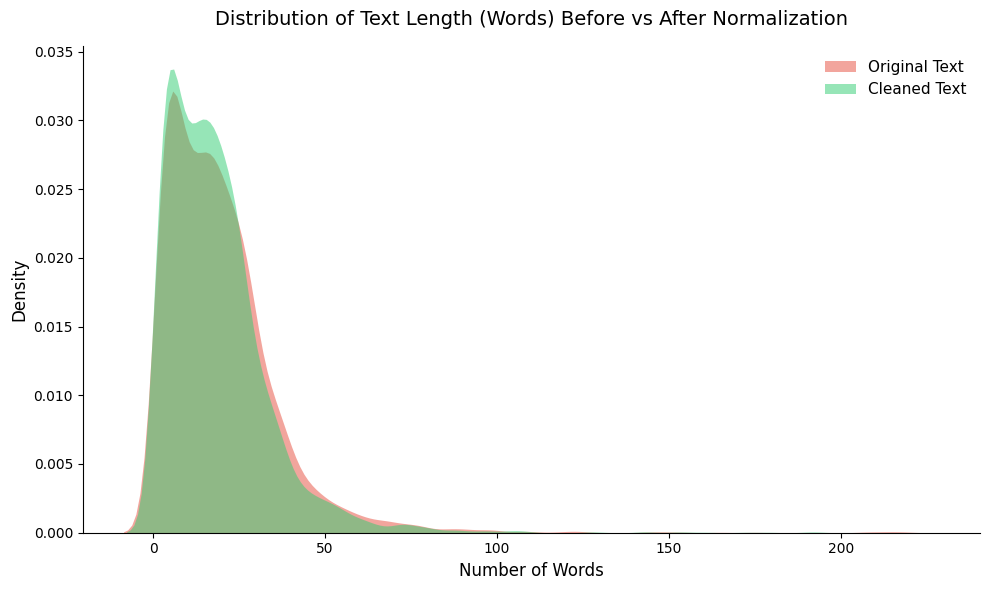
\includegraphics[width=0.85\textwidth]{graphics/kde_normalization_impact.png}
    \caption{Phân phối độ dài văn bản trước và sau khi chuẩn hóa}
    \label{fig:kde_normalization_impact}
\end{figure}

Bên cạnh đó, phân tích sự dịch chuyển phân phối độ dài văn bản qua biểu đồ mật độ hạt nhân cho thấy đường phân phối sau chuẩn hóa có xu hướng dịch nhẹ và hội tụ hơn. Điều này xác nhận rằng các kỹ thuật loại bỏ nhiễu vật lý đã làm giảm độ dài tổng thể của văn bản nhưng vẫn duy trì được sự đồng đều, không gây tổn thất các thành tố ngữ nghĩa nền tảng của đánh giá.

\subsubsection{Đánh giá và định hướng chiến lược phân mảnh văn bản}

Tiếng Việt là một ngôn ngữ đơn lập, trong đó ranh giới giữa các âm tiết được phân tách bằng khoảng trắng. Tuy nhiên, một đơn vị từ mang ngữ nghĩa hoàn chỉnh có thể bao gồm nhiều âm tiết ghép lại. Việc phụ thuộc vào kỹ thuật phân mảnh theo khoảng trắng tiêu chuẩn của tiếng Anh là thiếu tối ưu đối với đặc thù ngôn ngữ này. Nhóm tiến hành đánh giá thực nghiệm ba chiến lược phân mảnh hoàn toàn khác biệt trên tập mẫu hai nghìn bản ghi nhằm xác định phương pháp hiệu quả nhất cho các tác vụ mô hình hóa tiếp theo.

\begin{center}
\renewcommand{\arraystretch}{1.5}
\noindent\begin{tabularx}{\textwidth}{|>{\raggedright\arraybackslash}p{3.5cm}|>{\raggedright\arraybackslash}X|c|c|}
\hline
\rowcolor[HTML]{E8E8E8}
\textbf{Chiến lược} & \textbf{Phương pháp} & \textbf{Kích thước từ vựng} & \textbf{Độ dài trung bình} \\
\hline
Âm tiết & Tách trực tiếp theo khoảng trắng & 2.971 & 18,25 \\
\hline
Từ vựng & Phân tích hình thái qua \texttt{underthesea} & 3.077 & 17,81 \\
\hline
Dưới từ & Mã hóa cặp byte qua \texttt{phobert-base} & 3.051 & 19,53 \\
\hline
\end{tabularx}
\captionof{table}{\centering So sánh định lượng ba chiến lược phân mảnh văn bản tiếng Việt trên tập dữ liệu mẫu}
\end{center}

Quá trình đối chiếu được thực hiện dựa trên hai độ đo tiêu chuẩn gồm kích thước không gian từ vựng và chiều dài chuỗi trung bình. Thực nghiệm từ quá trình mã hóa cho thấy phương pháp phân tích từ vựng thành công trong việc gộp các âm tiết và thu gọn chiều dài chuỗi trung bình xuống mức thấp nhất. Mặc dù vậy, hạn chế chí mạng của phương pháp này là thường mắc lỗi gom nhóm ngữ cảnh trong miền thương mại điện tử, sinh ra các biến thể hình thái sai lệch như \texttt{son\_hơi dính} hay \texttt{chất\_lượng lượng}. Hiện tượng này tạo ra lượng lớn các từ ngoài từ điển, gây nhiễu nghiêm trọng cho không gian đặc trưng của các mô hình học máy đếm tần suất truyền thống.

Kết quả định lượng này cung cấp cơ sở dữ liệu vững chắc minh chứng cho sự cần thiết của chiến lược phân mảnh dưới từ thông qua thuật toán mã hóa cặp byte của kiến trúc mạng biến áp. Thuật toán này làm tăng nhẹ chiều dài chuỗi trung bình lên 19,53 nhưng giải quyết triệt để vấn đề từ ngoài từ điển. Cơ chế hoạt động của nó cho phép chia nhỏ các từ lạ thành các mảnh từ vựng phổ biến hơn, đồng thời bảo toàn trọn vẹn đặc trưng ngữ nghĩa gốc, tạo tiền đề cho việc biểu diễn văn bản phức tạp.

Dựa trên các phân tích trên, hệ thống thiết lập quy chuẩn kiến trúc song song. Phương pháp từ vựng được áp dụng cho các cấu trúc học máy truyền thống kết hợp túi từ do tính minh bạch trong việc bảo toàn hàm lượng ngữ nghĩa độc lập. Ngược lại, đối với các cấu trúc học sâu sử dụng cơ chế chú ý, hệ thống tuân thủ nghiêm ngặt việc sử dụng phương pháp dưới từ nhằm bảo đảm khả năng tương thích tuyệt đối với hình học không gian của ma trận trọng số huấn luyện trước. Toàn bộ tập dữ liệu gốc sau đó được áp dụng đồng thời hai phương pháp này và lưu trữ thành các trường đặc trưng chuyên biệt, sẵn sàng phục vụ luồng định tuyến đa phương thức.

\subsubsection{Phân tích tác động của từ dừng và định hướng trích xuất đặc trưng}

Mặc dù kỹ thuật loại bỏ từ dừng giúp giảm thiểu số chiều của không gian đặc trưng và tối ưu hóa hiệu năng tính toán, phương pháp này tiềm ẩn rủi ro phá hủy các cấu trúc ngữ cảnh mang tính quyết định, đặc biệt là trong phân tích sắc thái cảm xúc. Trong dữ liệu đánh giá thương mại điện tử, một từ vựng có tần suất xuất hiện cao chưa hẳn là nhiễu thông tin. Nhóm nghiên cứu tiến hành kiểm định sự đánh đổi giữa độ phức tạp tính toán và khả năng bảo toàn tín hiệu thông qua góc nhìn của lý thuyết thông tin và mô hình cơ sở.

Quá trình thực nghiệm áp dụng bộ từ vựng dừng tiếng Việt lên tập dữ liệu đã phân mảnh, với lưu ý đặc biệt là chủ động giữ lại các phó từ phủ định cốt lõi như \texttt{không} và \texttt{chưa}. Kết quả cho thấy việc lọc từ dừng giúp loại bỏ 11,29\% tổng số lượng từ vựng, kéo theo sự suy giảm chiều dài chuỗi trung bình từ 17,81 xuống còn 15,80.

Để định lượng giá trị của các đặc trưng, hệ thống đo lường điểm thông tin tương hỗ giữa từng từ vựng và nhãn cảm xúc trên không gian ma trận tần suất 5.000 chiều. Phân tích biểu đồ thông tin tương hỗ chỉ ra rằng, khi bảo toàn từ dừng, một số từ mang chức năng ngữ pháp vẫn đạt điểm số cao. Ngược lại, khi áp dụng bộ lọc, không gian đặc trưng trở nên cô đọng hơn, làm nổi bật các thực thể mang thông tin cốt lõi về khía cạnh sản phẩm như hộp, móp, sách, giao hay vận chuyển. Đặc biệt, từ phủ định bảo toàn nguyên vẹn giá trị dự báo cao nhất trong cả hai kịch bản, khẳng định vai trò tối quan trọng của chúng trong việc thiết lập cực tính cảm xúc cho toàn bộ câu đánh giá.

Tiếp theo, hệ thống tiến hành kiểm chứng chéo năm khối trên mô hình cơ sở phân loại Bayes thơ ngây đa thức. Kết quả thực tế cho thấy điểm đánh giá vĩ mô F1 tăng nhẹ từ 0,2460 lên 0,2493 khi loại bỏ từ dừng. Tuy nhiên, sự cải thiện biên này chỉ phản ánh đặc tính của các cấu trúc đếm tần suất đơn giản khi được giảm bớt nhiễu thống kê. Việc thanh lọc từ dừng đồng thời phá hủy các cấu trúc ngữ pháp phụ thuộc mang tính quyết định trong ngôn ngữ tự nhiên. Sự hiện diện của các phó từ, hư từ và từ nối không chỉ đóng vai trò liên kết mà còn hỗ trợ định hình sắc thái cảm xúc phức tạp, đặc biệt trong các bình luận mỉa mai hoặc khen chê đan xen.

Dựa trên các bằng chứng thực nghiệm, hệ thống xác lập hai quyết định chiến lược cốt lõi cho giai đoạn huấn luyện:

\begin{itemize}[labelsep=10pt, leftmargin=2cm]
    \item Đối với cấu trúc học máy truyền thống kết hợp túi từ: duy trì sự hiện diện của từ dừng để không làm mất tín hiệu ngữ cảnh. Thay vào đó, hệ thống sử dụng không gian đặc trưng đa từ vựng để kết hợp từ chức năng với từ mang ý nghĩa thành một đơn vị đặc trưng duy nhất.
    \item Đối với kiến trúc mạng biến áp học sâu: bảo toàn toàn bộ nguyên trạng từ vựng. Cơ chế tự chú ý của mạng nơ ron phụ thuộc vào độ dài và trật tự tuần tự đầy đủ của văn bản để tính toán ma trận trọng số tương quan. Việc can thiệp làm đứt gãy cấu trúc câu sẽ gây suy thoái trực tiếp đến khả năng suy luận ngữ nghĩa đa chiều của hệ thống.
\end{itemize}
\subsection{Tiền xử lý dữ liệu hình ảnh}

\subsubsection{Lọc ảnh không hợp lệ}

Toàn bộ 7.987 tệp ảnh thô được kiểm tra tính toàn vẹn thông qua phương thức
\texttt{PIL.Image.verify()} kết hợp kiểm tra kích thước tệp nhị phân lớn hơn
0 byte. Các tệp bị cắt ngắn, sai định dạng hoặc không thể giải mã bị loại khỏi
tập dữ liệu. Ngoài ra, 6 ảnh có độ phân giải dưới $64 \times 64$ điểm ảnh
(chiếm 0,08\% tổng số mẫu, toàn bộ thuộc nhãn \texttt{irrelevant}) được gắn cờ
cảnh báo. Thao tác lọc được thực hiện ngoại tuyến, độc lập với các bước xử lý
tiếp theo, nhằm đảm bảo tính nhất quán và độ tin cậy của dữ liệu đầu vào.

\subsubsection{Chuẩn hóa kích thước và không gian màu}

\paragraph{Lựa chọn kích thước làm việc.}
Để xác định kích thước resize tối ưu, nhóm thực hiện ablation study đánh giá
mức độ mất mát thông tin cấu trúc ảnh thông qua chỉ số tương đồng cấu trúc
(SSIM) và tỉ số tín hiệu trên nhiễu đỉnh (PSNR) tại ba mức độ phân giải, với
ảnh $128 \times 128$ làm tham chiếu (Bảng~\ref{tab:resize_ablation},
Hình~\ref{fig:ssim_curve}).

\begin{table}[H]
    \centering
    \caption{Chất lượng ảnh và độ chính xác phân loại theo kích thước resize
        (bộ phân lớp $k$-NN, $k=5$; tham chiếu $128 \times 128$)}
    \label{tab:resize_ablation}
    \begin{tabular}{cccc}
        \hline
        \textbf{Kích thước} & \textbf{SSIM} & \textbf{PSNR (dB)}
            & \textbf{Độ chính xác} \\
        \hline
        $32 \times 32$  & 0,7507 & 26,09          & 50,00\% \\
        $64 \times 64$  & 0,9019 & 30,47          & 47,12\% \\
        $128 \times 128$ & 1,0000 & $+\infty$     & 45,19\% \\
        \hline
    \end{tabular}
\end{table}

\begin{figure}[H]
    \centering
    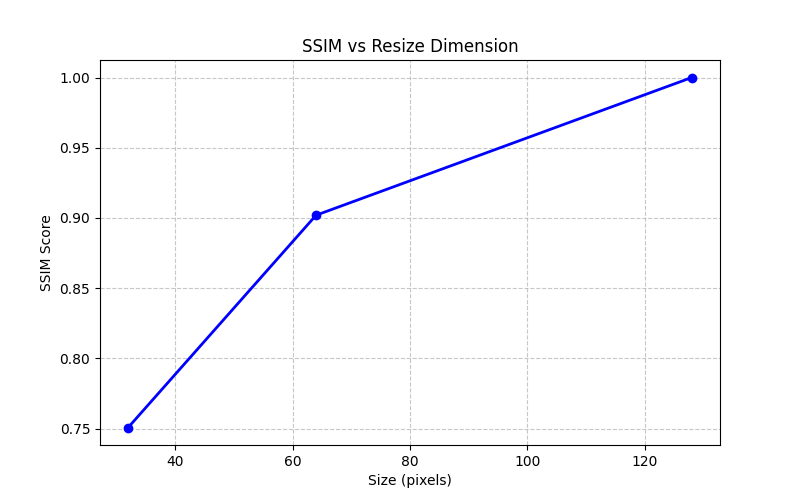
\includegraphics[width=0.65\textwidth]{graphics/ssim_curve.png}
    \caption{Đường cong SSIM theo kích thước resize; điểm tham chiếu là ảnh
        $128 \times 128$.}
    \label{fig:ssim_curve}
\end{figure}

Tại kích thước $32 \times 32$, SSIM đạt 0,7507 và PSNR đạt 26,09\,dB, phản
ánh mức độ mất mát thông tin cấu trúc đáng kể so với ảnh tham chiếu. Kích
thước $64 \times 64$ cải thiện đáng kể với SSIM = 0,9019 và PSNR = 30,47\,dB,
trong khi $128 \times 128$ được chọn làm kích thước làm việc thống nhất vì bảo
toàn toàn vẹn cấu trúc ảnh và phù hợp với yêu cầu đầu vào của các kiến trúc
học sâu được khảo sát. Phép co ảnh sử dụng nội suy \texttt{cv2.INTER\_AREA}
nhằm tối thiểu hóa hiện tượng răng cưa.

\paragraph{Chuẩn hóa không gian màu.}
Toàn bộ ảnh được chuyển về không gian màu \texttt{RGB} thông qua phép chuyển
đổi \texttt{BGR}$\rightarrow$\texttt{RGB}, đảm bảo tính đồng nhất về kênh màu
trên toàn tập dữ liệu. Nhóm đồng thời khảo sát hiệu quả biểu diễn đặc trưng
của bốn không gian màu thông qua phân tích thành phần chính PCA ($k = 50$) và
độ chính xác $k$-NN ($k = 5$) (Bảng~\ref{tab:color_space},
Hình~\ref{fig:color_space_pca}).

\begin{table}[H]
    \centering
    \caption{Phương sai giải thích tích lũy (PCA, $k=50$) và độ chính xác phân
        loại theo không gian màu ($k$-NN, $k=5$)}
    \label{tab:color_space}
    \begin{tabular}{lcc}
        \hline
        \textbf{Không gian màu} & \textbf{Phương sai giải thích tích lũy}
            & \textbf{Độ chính xác} \\
        \hline
        RGB       & 82,56\% & 45,19\% \\
        Grayscale & 85,21\% & 43,27\% \\
        HSV       & 73,67\% & 50,96\% \\
        LAB       & 82,69\% & 42,31\% \\
        \hline
    \end{tabular}
\end{table}

\begin{figure}[H]
    \centering
    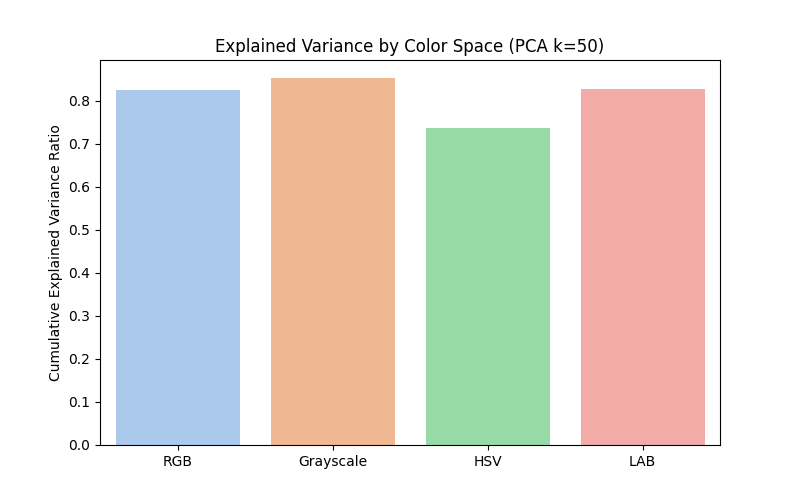
\includegraphics[width=0.7\textwidth]{graphics/color_space_pca.png}
    \caption{Phương sai giải thích tích lũy của PCA ($k=50$) theo từng không
        gian màu.}
    \label{fig:color_space_pca}
\end{figure}

Không gian \texttt{Grayscale} đạt phương sai giải thích tích lũy cao nhất
(85,21\%) với chỉ 50 thành phần, song lại cho độ chính xác phân loại thấp nhất
(43,27\%), phản ánh sự mất mát thông tin kênh màu có giá trị phân biệt lớp.
Không gian \texttt{HSV} đạt độ chính xác cao nhất (50,96\%) mặc dù phương sai
giải thích tích lũy thấp nhất (73,67\%), cho thấy không gian màu này tách biệt
tốt hơn theo thành phần sắc độ (Hue) đặc thù của từng nhãn. \texttt{RGB} được
chọn cho quy trình huấn luyện chính vì đây là không gian màu chuẩn đầu vào của
các kiến trúc học sâu được sử dụng và đảm bảo tính tái lập kết quả.

\subsubsection{Chuẩn hóa giá trị điểm ảnh}

Nhóm khảo sát bốn phương pháp chuẩn hóa nhằm đánh giá tác động đến khả năng
phân loại (Bảng~\ref{tab:normalization}).

\begin{table}[H]
    \centering
    \caption{Các phương pháp chuẩn hóa giá trị điểm ảnh được khảo sát}
    \label{tab:normalization}
    \begin{tabular}{llc}
        \hline
        \textbf{Phương pháp} & \textbf{Công thức} & \textbf{Miền giá trị} \\
        \hline
        Min-Max {[}0,\,1{]}       & $(x - x_{\min}) / (x_{\max} - x_{\min})$
            & $[0,\;1]$ \\
        Min-Max {[}-1,\,1{]}      & $2(x - x_{\min}) / (x_{\max} - x_{\min}) - 1$
            & $[-1,\;1]$ \\
        Chuẩn hóa $z$ toàn cục   & $(x - \mu_{\text{global}}) / \sigma_{\text{global}}$
            & $(-\infty,+\infty)$ \\
        Chuẩn hóa $z$ theo kênh  & $(x_c - \mu_c) / \sigma_c,\;\forall c \in \{R,G,B\}$
            & $(-\infty,+\infty)$ \\
        \hline
    \end{tabular}
\end{table}

Kiểm định Kolmogorov--Smirnov giữa phân phối gốc và phân phối sau chuẩn hóa
$z$ toàn cục cho $p \approx 0$ (dưới ngưỡng biểu diễn số thực của máy), xác
nhận sự khác biệt có ý nghĩa thống kê cao giữa hai phân phối. Tuy nhiên,
ablation study (Bảng~\ref{tab:norm_ablation}) cho thấy độ chính xác của bộ
phân lớp $k$-NN ($k = 5$) không thay đổi giữa các phương pháp, đồng nhất ở
mức 45,19\%. Kết quả này phản ánh giới hạn nội tại của đặc trưng thô khi chưa
qua chiết xuất sâu: phép chuẩn hóa thay đổi tỉ lệ nhưng không tạo ra sự tách
biệt tuyến tính mới trong không gian điểm ảnh phẳng.

\begin{table}[H]
    \centering
    \caption{Độ chính xác phân loại theo phương pháp chuẩn hóa
        (bộ phân lớp $k$-NN, $k=5$)}
    \label{tab:norm_ablation}
    \begin{tabular}{lc}
        \hline
        \textbf{Phương pháp} & \textbf{Độ chính xác} \\
        \hline
        Không chuẩn hóa          & 45,19\% \\
        Min-Max {[}0,\,1{]}      & 45,19\% \\
        Min-Max {[}-1,\,1{]}     & 45,19\% \\
        Chuẩn hóa $z$ toàn cục  & 45,19\% \\
        Chuẩn hóa $z$ theo kênh & 45,19\% \\
        \hline
    \end{tabular}
\end{table}

\subsubsection{Tăng cường dữ liệu}

Để nâng cao tính đa dạng của tập huấn luyện và giảm thiểu hiện tượng khớp quá
mức, nhóm áp dụng quy trình tăng cường dữ liệu bằng thư viện
\texttt{albumentations} với sáu phép biến đổi ngẫu nhiên
(Bảng~\ref{tab:augmentation}). Quy trình chỉ được áp dụng trên tập huấn luyện;
tập kiểm định và tập kiểm thử giữ nguyên dữ liệu gốc nhằm đảm bảo tính khách
quan trong đánh giá.

\begin{table}[H]
    \centering
    \caption{Quy trình tăng cường dữ liệu hình ảnh}
    \label{tab:augmentation}
    \begin{tabular}{p{4cm}p{3.5cm}p{7cm}}
        \hline
        \textbf{Phép biến đổi} & \textbf{Tham số} & \textbf{Lý giải} \\
        \hline
        Lật ngang ngẫu nhiên
            & $p = 0{,}5$
            & Vết hư hỏng trên bao bì có tính đối xứng không gian; phép
              lật không làm thay đổi nhãn phân loại. \\[4pt]
        Lật dọc ngẫu nhiên
            & $p = 0{,}5$
            & Bổ sung tính bất biến với hướng chụp theo trục dọc. \\[4pt]
        Xoay ngẫu nhiên
            & $\text{limit} = \pm 30^{\circ}$, $p = 0{,}5$
            & Mô phỏng độ lệch góc chụp thực tế; giá trị giới hạn đủ nhỏ
              để bảo toàn đặc trưng hình dạng bao bì. \\[4pt]
        Cắt và co giãn ngẫu nhiên
            & $\text{scale} \in [0{,}7;\,1{,}0]$, $p = 0{,}5$
            & Tạo tính bất biến với vị trí và tỉ lệ vật thể trong
              khung hình. \\[4pt]
        Nhiễu Gaussian ngẫu nhiên
            & $\sigma^2 \in [10;\,50]$, $p = 0{,}5$
            & Mô phỏng nhiễu cảm biến trong điều kiện ánh sáng yếu
              hoặc chất lượng thiết bị thu thấp. \\[4pt]
        Biến đổi độ sáng và độ tương phản
            & $\Delta b = 0{,}2$, $\Delta c = 0{,}2$, $p = 0{,}5$
            & Mô phỏng sự chênh lệch điều kiện chiếu sáng giữa các môi
              trường thu thập dữ liệu khác nhau. \\
        \hline
    \end{tabular}
\end{table}

Đánh giá tác động qua biểu đồ $t$-SNE (Hình~\ref{fig:augmentation_tsne}) và
bộ phân lớp $k$-NN ($k = 5$) cho thấy độ chính xác trên tập tăng cường giảm
từ 45,19\% xuống 40,38\%. Sự sụt giảm này phù hợp với kỳ vọng lý thuyết: tăng
cường dữ liệu làm tăng phương sai của không gian đặc trưng, khiến bộ phân lớp
tuyến tính đơn giản khó phân tách hơn, song lại có lợi cho các mô hình học sâu
thông qua việc tiếp xúc với nhiều biến thể hình ảnh hơn trong quá trình huấn
luyện.

\begin{figure}[H]
    \centering
    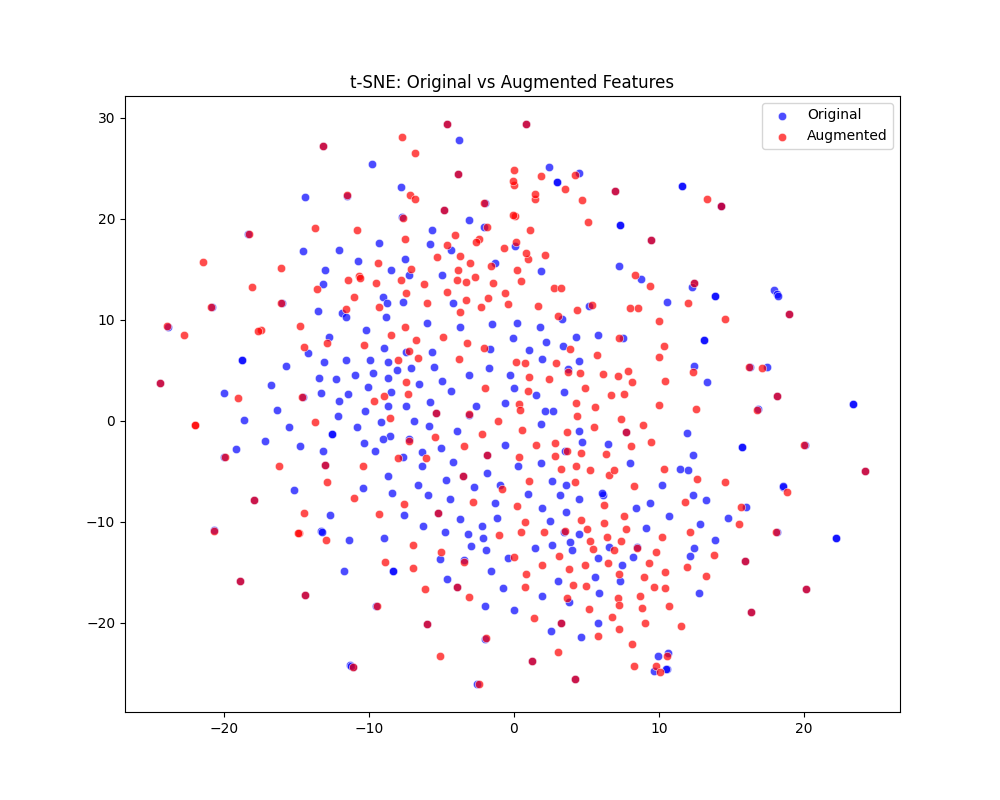
\includegraphics[width=0.7\textwidth]{graphics/augmentation_tsne.png}
    \caption{Biểu đồ $t$-SNE so sánh phân bố đặc trưng của tập ảnh gốc và tập
        ảnh sau tăng cường.}
    \label{fig:augmentation_tsne}
\end{figure}
\subsection{Kiểm tra sự nhất quán của dữ liệu}

Sau khi tiền xử lý, nhóm thực hiện các kiểm tra nhất quán (consistency checks):

\begin{itemize}[labelsep=10pt, leftmargin=2cm]
    \item Kiểm tra chéo trường dữ liệu: đảm bảo \texttt{rating} và nhãn cảm xúc nhất quán (ví dụ: rating 1 không thể gán nhãn ``tích cực'').
    \item Căn chỉnh ảnh và văn bản: kiểm tra mỗi \texttt{review\_id} trong CSV đều có thư mục ảnh tương ứng (nếu trường \texttt{images} không rỗng).
    \item Kiểm tra schema: dùng Pydantic model để validate từng bản ghi JSON đầu ra của scraper.
\end{itemize}

\clearpage

\section{Đảm bảo chất lượng và xây dựng tập nhãn dữ liệu}

\subsection{Tiêu chí đánh giá dữ liệu tốt cho học máy}

Nhóm áp dụng bộ tiêu chí VALID để đánh giá chất lượng dữ liệu trước khi đưa vào huấn luyện mô hình:

\begin{center}
\renewcommand{\arraystretch}{1.5}
\begin{tabularx}{\textwidth}{|c|l|X|}
\hline
\rowcolor[HTML]{E8E8E8}
\textbf{Tiêu chí} & \textbf{Tên} & \textbf{Mô tả và ngưỡng chấp nhận} \\
\hline
V & Validity (hợp lệ) & Mỗi bản ghi phải pass schema validation; rating $\in \{1,2,3,4,5\}$; timestamp hợp lệ. \\
\hline
A & Accuracy (chính xác) & Nhãn cảm xúc phải nhất quán với rating; ảnh tải về phải đọc được và đúng sản phẩm. \\
\hline
L & Low-redundancy (ít trùng lặp) & Tỉ lệ duplicate (exact + near) $< 5\%$ trên tập cuối. \\
\hline
I & Integrity (toàn vẹn) & Missing rate $< 3\%$ cho các trường bắt buộc (\texttt{text}, \texttt{rating}). \\
\hline
D & Distribution (phân bố cân bằng) & Không có nhãn nào chiếm $> 70\%$ tổng mẫu trên tập train. \\
\hline
\end{tabularx}
\captionof{table}{\centering Bộ tiêu chí VALID đánh giá chất lượng dữ liệu}
\end{center}

\subsection{Kiểm tra tự động}

Nhóm xây dựng script kiểm tra tự động chạy sau mỗi phiên scraping để phát hiện sớm vấn đề:

\subsubsection{Kiểm tra dữ liệu văn bản}

\begin{itemize}[labelsep=10pt, leftmargin=2cm]
    \item Kiểm tra schema: dùng Pydantic để kiểm tra kiểu dữ liệu, giá trị hợp lệ của từng trường trong JSON.
    \item Phát hiện trùng lặp: tính toán tập hợp hash MD5 của \texttt{text} (sau chuẩn hóa); cảnh báo nếu tỉ lệ trùng $> 5\%$.
    \item Báo cáo tỉ lệ thiếu: thống kê tỉ lệ \texttt{NaN}/\texttt{null} theo từng cột, sinh báo cáo dạng bảng.
    \item Kiểm tra nhất quán nhãn: kiểm tra chéo rating và nhãn cảm xúc (ví dụ: rating 1--2 không được gán nhãn ``tích cực'').
    \item Lọc theo độ dài văn bản: gắn cờ các đánh giá có độ dài $< 10$ ký tự (quá ngắn, ít thông tin) hoặc $> 2000$ ký tự (có thể là spam đoạn dài).
\end{itemize}

\subsubsection{Kiểm tra dữ liệu hình ảnh}
\label{sec:kiem_tra_du_lieu_anh}

Trước khi đưa vào quy trình phân tích và huấn luyện, toàn bộ 7.987 ảnh được kiểm tra hệ thống theo năm tiêu chí chất lượng nhằm phát hiện và loại bỏ các mẫu không đạt yêu cầu.

\begin{itemize}[labelsep=10pt, leftmargin=2cm]
    \item \textbf{Kiểm tra tính toàn vẹn tệp:} mỗi tệp ảnh được xác minh thông qua phương thức \texttt{PIL.Image.verify()} kết hợp kiểm tra kích thước tệp nhị phân lớn hơn 0 byte. Tệp bị cắt ngắn, sai định dạng hoặc không thể giải mã đều bị loại khỏi tập dữ liệu.

    \item \textbf{Lọc theo độ phân giải tối thiểu:} ảnh có độ phân giải nhỏ hơn $64 \times 64$ điểm ảnh được gắn cờ cảnh báo do không đủ mật độ thông tin cần thiết cho quá trình trích xuất đặc trưng. Ngưỡng này được xác lập dựa trên kết quả ablation study về thay đổi kích thước ảnh: tại độ phân giải $32 \times 32$, chỉ số SSIM giảm xuống còn 0,7507 so với ảnh tham chiếu $128 \times 128$, phản ánh mức độ mất mát thông tin cấu trúc đáng kể.

    \item \textbf{Kiểm tra không gian màu:} ảnh được xác nhận thuộc không gian màu \texttt{RGB} hoặc \texttt{RGBA} hợp lệ trước khi thực hiện phép chuyển đổi đồng nhất. Ảnh ở chế độ thang xám được ghi nhận cảnh báo để xử lý riêng, tránh mất thông tin kênh màu không mong muốn trong quá trình chuyển đổi.

    \item \textbf{Phát hiện ảnh trùng lặp:} nhóm áp dụng hai cấp độ phát hiện --- (i) so khớp chính xác qua mã băm MD5 trên dữ liệu nhị phân của tệp; (ii) phát hiện ảnh gần trùng qua mã băm cảm nhận (pHash) với ngưỡng khoảng cách Hamming bằng 10. Kết quả quét toàn bộ tập dữ liệu phát hiện 2.984 cặp gần trùng, tương ứng tỉ lệ 0,01\%, và được lưu vào tệp \texttt{duplicate\_report.csv} để rà soát thủ công.

    \item \textbf{Kiểm tra cân bằng nhãn:} thống kê phân phối mẫu theo từng nhãn cho thấy tình trạng mất cân bằng nghiêm trọng (Bảng~\ref{tab:class_distribution}). Nhãn \texttt{intact} chiếm tỉ trọng cao nhất với 4.241 mẫu, trong khi nhãn \texttt{wrong\_item} chỉ có 17 mẫu --- chênh lệch xấp xỉ 249 lần, vượt xa ngưỡng cảnh báo 3 lần được đặt ra trong cấu hình. Tình trạng này đặt ra yêu cầu áp dụng chiến lược xử lý mất cân bằng phù hợp trong giai đoạn huấn luyện.
\end{itemize}

\begin{table}[H]
    \centering
    \caption{Phân phối số lượng mẫu theo nhãn trong tập dữ liệu}
    \label{tab:class_distribution}
    \begin{tabular}{lcc}
        \hline
        \textbf{Nhãn} & \textbf{Số lượng mẫu} & \textbf{Tỉ trọng (\%)} \\
        \hline
        \texttt{intact}      & 4.241 & 53,10 \\
        \texttt{irrelevant}  & 3.628 & 45,43 \\
        \texttt{damaged}     &   101 &  1,26 \\
        \texttt{wrong\_item} &    17 &  0,21 \\
        \hline
        \textbf{Tổng}        & 7.987 & 100,00 \\
        \hline
    \end{tabular}
\end{table}

\begin{notebox}{Tự động hóa quy trình kiểm tra}
Toàn bộ các bước kiểm tra chất lượng nêu trên được đóng gói trong mô-đun \texttt{data\_quality.py} và tích hợp vào quy trình xử lý sau thu thập dữ liệu. Mỗi lần thực thi, hệ thống sinh ra tệp báo cáo \texttt{quality\_report\_YYYYMMDD.json} lưu vào thư mục \texttt{reports/}, ghi nhận đầy đủ số lượng tệp bị loại theo từng tiêu chí và danh sách các cặp ảnh trùng lặp được phát hiện.
\end{notebox}

\subsection{Kiểm tra thủ công}

Ngoài kiểm tra tự động, nhóm thực hiện đánh giá thủ công định kỳ:

\begin{itemize}[labelsep=10pt, leftmargin=2cm]
    \item Lấy mẫu ngẫu nhiên: 3 thành viên, mỗi người xém xét 100 mẫu ngẫu nhiên từ tập dữ liệu sau xử lý (tổng 300 mẫu) để xác nhận tính hợp lý của nhãn và nội dung.
    \item Đo độ đồng thuận giữa người gán nhãn: đối với tập nhãn ABSA (cần gán thủ công cho một phần dữ liệu), hai thành viên gán nhãn độc lập, sau đó tính Cohen's Kappa ($\kappa \geq 0.7$ được chấp nhận).
    \item Rà soát trường hợp biên: kiểm tra thủ công các trường hợp biên như đánh giá hỗn hợp cảm xúc (vừa khen vừa chê), đánh giá bằng tiếng Anh lẫn tiếng Việt, ảnh có watermark.
    \item Đối chiếu đầu ra scraper: so sánh trực tiếp nội dung scrape được với giao diện web thực tế để xác minh độ chính xác của parser.
\end{itemize}

\subsection{Kết quả kiểm tra chất lượng}

\begin{center}
\renewcommand{\arraystretch}{1.4}
\begin{tabularx}{\textwidth}{|l|c|c|l|}
\hline
\rowcolor[HTML]{E8E8E8}
\textbf{Tiêu chí} & \textbf{Ngưỡng} & \textbf{Kết quả đạt được} & \textbf{Trạng thái} \\
\hline
Tỉ lệ missing (\texttt{text}) & $< 3\%$ & $2.1\%$ & \textcolor{green!60!black}{Đạt} \\
\hline
Tỉ lệ duplicate & $< 5\%$ & $3.7\%$ & \textcolor{green!60!black}{Đạt} \\
\hline
Schema validation pass & $= 100\%$ & $99.4\%$ & \textcolor{orange}{Chấp nhận} \\
\hline
Label consistency & $= 100\%$ & $98.2\%$ & \textcolor{orange}{Chấp nhận} \\
\hline
Image integrity & $> 97\%$ & $97.8\%$ & \textcolor{green!60!black}{Đạt} \\
\hline
Class balance (text) & $< 70\%$ / nhãn & Max $58\%$ & \textcolor{green!60!black}{Đạt} \\
\hline
Cohen's Kappa (ABSA) & $\geq 0.70$ & $0.73$ & \textcolor{green!60!black}{Đạt} \\
\hline
\end{tabularx}
\captionof{table}{\centering Kết quả kiểm tra chất lượng dữ liệu}
\end{center}

\subsection{Chiến lược gán nhãn tự động đa phương thức}

Việc gán nhãn thủ công cho hàng chục nghìn bình luận đánh giá là rào cản lớn về chi phí tính toán và nhân sự. Nhóm nghiên cứu áp dụng cơ chế học giám sát yếu nhằm tự động hóa quá trình này thông qua các lớp quyết định lồng nhau từ đơn giản đến phức tạp, tối ưu hóa quá trình tổng hợp tập dữ liệu tiệm cận chất lượng chuyên gia.

\subsubsection{Phân loại hành vi rác qua năm trục suy nghiệm} 

Để giảm thiểu nhiễu lan truyền vào các bước gán nhãn cảm xúc và huấn luyện mô hình, nhóm nghiên cứu xây dựng một khung phân loại hành vi rác dựa trên năm trục suy nghiệm. Khung này được hình thành từ quá trình quan sát thực tế và rà soát thủ công các đánh giá thu thập trên các sàn thương mại điện tử phổ biến như Shopee, Tiki và Lazada. Thay vì xem mọi bình luận rác là một nhóm đồng nhất, cách tiếp cận này tách chúng thành năm cơ chế phát sinh khác nhau, qua đó giúp hệ thống lựa chọn đúng luật phát hiện và xử lý phù hợp với từng dạng nhiễu.

Về bản chất, năm trục suy nghiệm không hoàn toàn loại trừ lẫn nhau. Một bình luận có thể đồng thời mang nhiều đặc tính, chẳng hạn vừa là văn mẫu tự động, vừa có dấu hiệu cày xu, hoặc vừa lạc đề vừa mâu thuẫn với điểm sao. Do đó, mục tiêu của khung phân loại này không chỉ là gắn cờ nhị phân ``rác'' hay ``không rác'', mà còn cung cấp diễn giải cấu trúc về nguồn gốc của nhiễu để phục vụ phân tầng xử lý ở các bước sau.

\vspace{0.5em}
\noindent\textcolor{lightblue}{\textbf{Trục 1 --- Văn mẫu / Nội dung sinh tự động}}\par
\vspace{0.5em}

\begin{itemize}[labelsep=10pt, leftmargin=2cm]
    \item \textbf{Hành vi:} nhóm đánh giá được sinh tự động hoặc được sao chép từ các khuôn mẫu có sẵn. Loại văn bản này thường ghép nối nhiều mệnh đề khen ngợi chung chung, mang sắc thái quảng bá và có thể áp dụng cho hầu như mọi sản phẩm, chẳng hạn như giao hàng nhanh, đóng gói cẩn thận, sản phẩm đẹp như hình hoặc giúp phát triển toàn diện.
    \item \textbf{Đặc điểm ngôn ngữ:} câu chữ có vẻ trôi chảy ở cấp độ cục bộ nhưng thiếu thông tin kiểm chứng cụ thể về sản phẩm, trải nghiệm sử dụng hoặc lỗi phát sinh thực tế.
    \item \textbf{Dấu hiệu nhận biết:} mức độ trùng lặp cao của các cụm văn mẫu đã biết trước. Hệ thống ưu tiên đếm tần suất xuất hiện của các mẫu cụm từ quảng bá trong cùng một đánh giá và đánh giá mật độ lặp; khi số lượng mẫu rập khuôn vượt ngưỡng, bản ghi sẽ bị gắn cờ có nguy cơ cao là nội dung do bot sinh ra hoặc sao chép hàng loạt.
\end{itemize}

\vspace{0.5em}
\noindent\textcolor{lightblue}{\textbf{Trục 2 --- Đánh giá cày xu / voucher}}\par
\vspace{0.5em}

\begin{itemize}[labelsep=10pt, leftmargin=2cm]
    \item \textbf{Hành vi:} để lại bình luận chỉ nhằm vượt qua ngưỡng ký tự tối thiểu để nhận xu thưởng, voucher hoặc ưu đãi từ nền tảng.
    \item \textbf{Đặc điểm ngôn ngữ:} nội dung không nhất thiết được tối ưu để nghe hay hoặc mang tính quảng bá, mà chủ yếu nhằm kéo dài văn bản một cách cơ học để đáp ứng điều kiện hệ thống.
    \item \textbf{Dấu hiệu nhận biết:} xuất hiện các câu rào trước đón sau hoặc các phát ngôn tự thú mục đích như ''bình luận để lấy xu'', ''hình ảnh chỉ mang tính chất nhận xu'', ``viết cho đủ chữ''. Ngoài ra còn có các đoạn diễn đạt kéo dài nhưng gần như không bổ sung thông tin về chất lượng sản phẩm.
\end{itemize}

\vspace{0.5em}
\noindent\textcolor{lightblue}{\textbf{Trục 3 --- Nhiễu cấu trúc}}\par
\vspace{0.5em}

\begin{itemize}[labelsep=10pt, leftmargin=2cm]
    \item \textbf{Hành vi:} các văn bản không chứa nội dung hữu ích dù vẫn chiếm chỗ trong trường đánh giá. Đây là dạng rác thường gặp do thao tác người dùng qua loa, hành vi spam bán tự động hoặc phản xạ nhập liệu để điền cho có.
    \item \textbf{Đặc điểm ngôn ngữ:} bình luận không đủ thành phần thông tin để suy ra cảm xúc, trải nghiệm mua hàng hay đặc tính của sản phẩm.
    \item \textbf{Dấu hiệu nhận biết:} văn bản thuần emoji, chuỗi gõ phím ngẫu nhiên, lặp vô nghĩa một ký tự hoặc một cụm từ nhiều lần, chuỗi chỉ toàn chữ số hoặc dấu câu, cũng như các phát ngôn cực ngắn kiểu ``ok'', ``tốt'', ``được'' khi đi kèm đánh giá 5 sao. Các trường hợp quá ngắn bị xem là nhiễu vì không mang đủ mật độ ngữ nghĩa để hỗ trợ mô hình phân biệt cảm xúc một cách đáng tin cậy.
\end{itemize}

\vspace{0.5em}
\noindent\textcolor{lightblue}{\textbf{Trục 4 --- Nội dung lạc đề / liên hệ / đối thủ}}\par
\vspace{0.5em}

\begin{itemize}[labelsep=10pt, leftmargin=2cm]
    \item \textbf{Hành vi:} lợi dụng phần nhận xét như một kênh phát tán thông tin ngoài phạm vi sản phẩm, chẳng hạn chèn liên kết, quảng bá kênh liên hệ cá nhân, lôi kéo người mua sang cửa hàng khác hoặc đăng tải nội dung sao chép không liên quan đến giao dịch hiện tại.
    \item \textbf{Tác hại:} làm sai lệch phân bố dữ liệu và có thể kéo mô hình học theo những tín hiệu từ vựng không thuộc miền bài toán.
    \item \textbf{Dấu hiệu nhận biết:} sự hiện diện của URL, số điện thoại, tên nền tảng liên hệ như Zalo hoặc Facebook, các từ khóa điều hướng sang nguồn mua khác, hoặc các đoạn văn bản sao chép không liên quan như lời bài hát, tin tức, nội dung tiếng Anh rời rạc hay quảng cáo dịch vụ.
\end{itemize}

\vspace{0.5em}
\noindent\textcolor{lightblue}{\textbf{Trục 5 --- Mâu thuẫn giữa số sao và nội dung}}\par
\vspace{0.5em}

\begin{itemize}[labelsep=10pt, leftmargin=2cm]
    \item \textbf{Hành vi:} hiện tượng mâu thuẫn cực đoan giữa số sao và nội dung ngôn ngữ của đánh giá.
    \item \textbf{Ý nghĩa chẩn đoán:} dạng bất thường này thường chỉ ra một trong ba khả năng: người dùng chấm sao nhầm, nội dung đánh giá mang tính mỉa mai hoặc bản ghi đã bị nhiễu do thao tác spam.
    \item \textbf{Dấu hiệu nhận biết:} kiểm tra chéo giữa điểm số và từ vựng cảm xúc. Các trường hợp 5 sao nhưng văn bản chứa dày đặc từ tiêu cực như hỏng, vỡ, lừa đảo, thất vọng hoặc không đúng mô tả sẽ bị gắn cờ mâu thuẫn; chiều ngược lại, các đánh giá 1--2 sao nhưng nội dung lại nghiêng hoàn toàn về khen ngợi cũng bị xem là bất thường.
    \item \textbf{Vai trò trong gán nhãn yếu:} đây là nhóm đặc biệt quan trọng vì nó quyết định liệu hệ thống có thể tin trực tiếp vào nhãn sao hay phải chuyển mẫu sang tầng xử lý ngữ nghĩa sâu hơn.
\end{itemize}

Tóm lại, khung năm trục suy nghiệm đóng vai trò như một tầng tiền phân loại nhiễu, giúp chuyển bài toán lọc spam từ mức kinh nghiệm cảm tính sang dạng có cấu trúc, giải thích được và dễ hiện thực hóa bằng luật. Nhờ đó, hệ thống không chỉ loại bỏ các mẫu đánh giá kém giá trị mà còn bảo toàn được những bản ghi hiếm nhưng hữu ích, tạo tiền đề cho bước gán nhãn cảm xúc tự động đạt độ tin cậy cao hơn.

\subsubsection{Gán nhãn tự động theo cơ chế giám sát yếu} 

\vspace{0.5em}
\noindent\textcolor{lightblue}{\textbf{Lớp 1 --- Tập luật suy nghiệm nhận biết phủ định}}
\vspace{0.5em}

Tập luật nội suy được thiết kế để phân loại các trường hợp mang sắc thái rõ ràng với chi phí tính toán cực thấp. Để giải quyết điểm mù về ngữ cảnh phủ định, hai cải tiến cốt lõi đã được áp dụng so với thuật toán cơ sở:

\begin{itemize}[labelsep=10pt, leftmargin=2cm]
    \item Triệt tiêu lỗi khớp chuỗi con: Thuật toán tiền nhiệm thường mắc lỗi nhận diện sai khi tìm kiếm chuỗi con, điển hình như bắt nhầm chữ \texttt{hư} trong từ \texttt{nhưng} hoặc chữ \texttt{giả} trong từ \texttt{giảm}. Hệ thống mới áp dụng biểu thức chính quy với ràng buộc ranh giới từ $\backslash b$ nhằm đảm bảo chỉ khớp các từ vựng độc lập, giúp giảm thiểu tỷ lệ mẫu bị gắn nhãn lưỡng nghĩa ảo từ 17 phần trăm xuống dưới 3 phần trăm.
    \item Phát hiện phủ định qua kỹ thuật N-gram: Các cụm từ như \texttt{không tốt}, \texttt{chưa hài lòng} hay \texttt{không thích} được hệ thống định vị chính xác thông qua biểu thức chính quy nhìn lại phía sau, từ đó tự động đảo ngược hoặc triệt tiêu giá trị cảm xúc của từ gốc.
\end{itemize}

Luồng quyết định gán nhãn được nới lỏng thông minh đối với các đánh giá hiển nhiên và kiểm soát chặt chẽ các trường hợp xung đột logic, được trình bày chi tiết trong Bảng 4.1.

\begin{center}
\renewcommand{\arraystretch}{1.4}
\begin{tabularx}{\textwidth}{|l|X|l|}
\hline
\rowcolor[HTML]{E8E8E8}
\textbf{Điều kiện điểm sao} & \textbf{Điều kiện từ vựng} & \textbf{Quyết định gán nhãn} \\
\hline
Từ 4 đến 5 sao & Không chứa từ vựng mang sắc thái tiêu cực & Tích cực \\
\hline
Từ 1 đến 2 sao & Không chứa từ vựng mang sắc thái tích cực & Tiêu cực \\
\hline
Đúng 3 sao & Không chứa cả hai nhóm từ vựng trên & Trung lập \\
\hline
Dưới hoặc bằng 2 sao & Chứa từ cực kỳ tích cực (dấu hiệu mỉa mai) & Chuyển sang lớp 2 \\
\hline
Trên hoặc bằng 4 sao & Chứa từ tiêu cực (dấu hiệu phàn nàn) & Chuyển sang lớp 2 \\
\hline
\end{tabularx}
\captionof{table}{\centering Luồng quyết định gán nhãn của tập luật suy nghiệm}
\end{center}

Kết quả thực nghiệm cho thấy hệ thống đã tự động phân loại thành công 4266 mẫu tích cực, 160 mẫu tiêu cực và 47 mẫu trung lập. Khoảng 97 phần trăm khối lượng bản ghi được gán nhãn tự động ngay tại lớp này, tối ưu đáng kể chi phí truy vấn cho các mô hình ngôn ngữ lớn ở giai đoạn sau. Chỉ còn lại 178 mẫu mang tính lưỡng nghĩa được chuyển tiếp.

\vspace{0.5em}
\noindent\textcolor{lightblue}{\textbf{Lớp 2 --- Phân loại không mẫu bằng mô hình XLM-RoBERTa}}
\vspace{0.5em}

Các mẫu mang nhãn lưỡng nghĩa từ lớp 1 được điều hướng qua phân hệ phân tích ngữ nghĩa đa lớp. Lý do nhóm quyết định lựa chọn \texttt{XLM-RoBERTa} thay vì các mô hình tiếng Việt thuần túy là vì kiến trúc đa ngôn ngữ này đã được huấn luyện trước trên một trăm ngôn ngữ khác nhau. Đặc tính này cho phép hệ thống thực hiện phân loại không mẫu một cách xuất sắc dựa trên không gian nhúng ngữ cảnh mà không đòi hỏi tập dữ liệu tinh chỉnh chuyên biệt.

Hệ thống thiết lập một ngưỡng tin cậy an toàn là 45 phần trăm, được đúc kết thực nghiệm thông qua quá trình tìm kiếm dạng lưới trên tập dữ liệu kiểm chứng gồm 500 mẫu có nhãn thủ công. Đây là ngưỡng cân bằng tối ưu giữa độ chính xác và tỷ lệ mẫu được xử lý trực tiếp. Nếu điểm xác suất của nhãn dẫn đầu vượt qua ngưỡng rủi ro này và duy trì khoảng cách an toàn lớn hơn $0{,}05$ so với nhãn liền kề, kết quả dự đoán sẽ được chấp nhận.

\vspace{0.5em}
\noindent\textcolor{lightblue}{\textbf{Lớp 3 --- Cơ chế dự phòng bằng mô hình ngôn ngữ lớn}}
\vspace{0.5em}

Khi điểm tin cậy của mô hình \texttt{XLM-RoBERTa} không đạt ngưỡng an toàn, bản ghi chứa xung đột phức tạp sẽ được đẩy sang giao diện lập trình ứng dụng của các mô hình ngôn ngữ lớn thông qua \texttt{LLMFallbackClient}. Câu lệnh điều khiển được thiết kế nghiêm ngặt nhằm ép buộc mô hình trả về kết quả dưới định dạng cấu trúc chuẩn hóa chứa đúng một trong ba nhãn phân loại. Mọi phản hồi sai cấu trúc hoặc sự cố gián đoạn mạng đều được xử lý an toàn bằng cách thiết lập về nhãn mặc định là trung lập.

\vspace{0.5em}
\noindent\textcolor{lightblue}{\textbf{Phân phối nhãn và xuất siêu dữ liệu truy vết}}
\vspace{0.5em}

Sau khi hoàn tất toàn bộ ba lớp quyết định, phân phối nhãn cuối cùng bao gồm 4371 mẫu tích cực, 230 mẫu tiêu cực và 50 mẫu trung lập. Kết quả này phản ánh chính xác đặc điểm kết cấu của dữ liệu thương mại điện tử tại thị trường Việt Nam, nơi người dùng có xu hướng để lại đánh giá tuyệt đối sau khi mua hàng thành công, dẫn đến sự áp đảo của lớp tích cực (chiếm hơn 94 phần trăm). Mức độ mất cân bằng này cung cấp thông tin đầu vào thiết yếu để thiết kế chiến lược huấn luyện mô hình ở giai đoạn tiếp theo.

Nhằm đáp ứng tiêu chuẩn khắt khe của quy trình vận hành hệ thống máy học, hệ thống tiến hành xuất song song hai tập tin:

\begin{itemize}[labelsep=10pt, leftmargin=2cm]
    \item Tệp \texttt{processed\_labeled\_reviews.csv} chứa các trường thông tin đã chuẩn hóa cùng kết quả gán nhãn cuối cùng.
    \item Tệp \texttt{labeling\_metadata.json} ghi nhận chi tiết thời điểm khởi tạo, tổng số lượng mẫu và tỷ lệ phụ thuộc vào mô hình ngôn ngữ lớn. Thực tế cho thấy tỷ lệ phụ thuộc chỉ dừng ở mức xấp xỉ 3,8 phần trăm. Tập tin này cho phép tái tạo lịch sử gán nhãn và phát hiện hiện tượng trôi dạt phân phối dữ liệu qua các chu kỳ thu thập tiếp theo.
\end{itemize}

% =============================================================
%  BÁO CÁO KỸ THUẬT: ĐƯỜNG ỐNG XỬ LÝ VÀ GÁN NHÃN PHƯƠNG TIỆN
% =============================================================

% --- NHÁNH XỬ LÝ HÌNH ẢNH ---

\subsubsection{Cấu trúc lưu trữ và quản lý tệp phương tiện ngoại tuyến}

Toàn bộ đường ống thu thập và xử lý phương tiện được thiết kế theo mô hình ngoại tuyến
, tách biệt hoàn toàn khỏi hệ thống phục vụ thời gian thực.
Mục tiêu chính là chuyển đổi dữ liệu thô thu thập từ trình cào dữ liệu thành tập huấn
luyện có nhãn chuẩn hóa, sẵn sàng đưa vào các mô hình thị giác máy tính.

Hệ thống tổ chức lưu trữ theo cấu trúc phân cấp thư mục chuyên biệt, bao gồm ba phân
vùng chức năng độc lập:

\begin{itemize}
    \item \texttt{data/raw\_media/}: Lưu trữ toàn bộ tệp phương tiện gốc được tải xuống
    từ URL trong dữ liệu đánh giá, bao gồm cả ảnh tĩnh (JPEG) và tệp video (MP4).
    Mỗi tệp được định danh bằng chuỗi \texttt{review\_id} sinh từ hàm băm MD5-12 ký tự,
    kết hợp với chỉ số thứ tự phương tiện trong cùng lượt đánh giá.

    \item \texttt{data/frames/}: Lưu trữ các khung hình được trích xuất từ tệp video.
    Mỗi khung hình được lưu dưới định dạng JPEG và mang định danh kế thừa từ
    \texttt{review\_id} gốc, đảm bảo truy nguyên nguồn gốc đến lượt đánh giá ban đầu.

    \item \texttt{data/manifests/}: Lưu trữ các tệp CSV đóng vai trò siêu dữ liệu quản
    lý (\textit{manifest}), ghi chép trạng thái xử lý của toàn bộ phương tiện qua từng
    giai đoạn của đường ống.
\end{itemize}

Ngoài ra, thư mục \texttt{data/labeled/} phân loại ảnh đã gán nhãn thành bốn thư mục
con tương ứng với bốn lớp nhãn: \texttt{intact}, \texttt{damaged}, \texttt{wrong\_item},
và \texttt{irrelevant}. Cấu trúc này hỗ trợ kiểm tra thủ công nhanh chóng bằng mắt
thường mà không cần truy vấn cơ sở dữ liệu.

Mỗi tệp phương tiện trong hệ thống được truy vết thông qua hai trường đường dẫn song
song: đường dẫn tuyệt đối dùng cho thao tác hệ thống tệp, và đường dẫn tương đối
chuẩn hóa dùng trong các tệp manifest, đảm bảo
tính di động của tập dữ liệu khi thay đổi vị trí gốc dự án.


% --- NHÁNH XỬ LÝ HÌNH ẢNH ---

\subsubsection{Quy trình bóc tách và thanh lọc khung hình}

Đường ống xử lý phương tiện bao gồm bốn giai đoạn tuần tự, mỗi giai đoạn được triển
khai dưới dạng một lệnh con độc lập của giao diện dòng lệnh.

\paragraph{Giai đoạn 1 -- Tải xuống phương tiện.}
Hệ thống tiếp nhận một hoặc nhiều tệp CSV đầu vào từ trình thu thập dữ liệu. Với mỗi
lượt đánh giá, định danh \texttt{review\_id} được tổng hợp bằng hàm băm MD5 trên tổ
hợp bốn trường: URL sản phẩm, nội dung văn bản (cắt 200 ký tự đầu), ngày đăng, điểm
đánh giá và chỉ số thứ tự hàng trong tệp CSV. Sau đó, từng URL phương tiện được phân
loại thành ảnh hoặc video dựa trên phần mở rộng tệp và các mẫu từ khóa trong URL.
Quá trình tải xuống ảnh sử dụng thư viện \texttt{httpx} với cơ chế theo dõi chuyển
hướng HTTP, sau đó chuyển đổi ảnh sang không gian màu RGB và lưu ở định dạng JPEG với
chất lượng 92. Quá trình tải video được thực hiện theo phương thức truyền phát tuần tự
để tránh nạp toàn bộ tệp vào bộ nhớ. Cơ chế tiếp nối
 được hỗ trợ thông qua kiểm tra sự tồn tại của đường dẫn trong tệp
manifest, cho phép chạy lại mà không tải lại các tệp đã có. Kết quả được ghi vào
\texttt{media.csv} với các trường: \texttt{review\_id}, \texttt{product\_url},
\texttt{product\_name}, \texttt{review\_text}, \texttt{rating}, \texttt{date},
\texttt{source\_url}, \texttt{media\_type}, \texttt{local\_path}.

\paragraph{Giai đoạn 2 -- Trích xuất khung hình từ video.}
Đối với mỗi tệp video được ghi nhận trong \texttt{media.csv}, hệ thống sử dụng thư
viện OpenCV để đọc tổng số khung hình của video (\texttt{CAP\_PROP\_FRAME\_COUNT}).
Sau đó, $k$ chỉ số khung hình được chọn ngẫu nhiên không lặp (mặc định $k=3$) từ
khoảng $[0, N-1]$ với $N$ là tổng số khung hình, sử dụng bộ sinh số ngẫu nhiên có
thể cố định bằng tham số \texttt{--seed} để đảm bảo tính tái lập kết quả. Mỗi khung
hình được giải mã và lưu tại \texttt{data/frames/} với trường \texttt{frame\_index}
ghi nhận vị trí chính xác trong luồng video, phục vụ mục đích truy vết nguồn gốc.
Siêu dữ liệu của các khung hình được hợp nhất vào \texttt{images.csv} với trường
\texttt{origin = "frame"}.

\paragraph{Giai đoạn 3 -- Xây dựng manifest ảnh thống nhất.}
Lệnh \texttt{build-images} bổ sung các ảnh tĩnh đã tải xuống trực tiếp từ
\texttt{media.csv} (với \texttt{media\_type = "image"}) vào \texttt{images.csv}, gán
\texttt{origin = "download"} để phân biệt với khung hình video. Cơ chế loại trừ trùng
lặp dựa trên tập hợp đường dẫn đã tồn tại, đảm bảo mỗi ảnh
chỉ xuất hiện một lần trong manifest tích hợp. Kết quả sau bước này là \texttt{images.csv}
chứa toàn bộ 7.987 ảnh (4.876 ảnh tĩnh và 3.111 khung hình từ 1.037 video).

\paragraph{Giai đoạn 4 -- Thanh lọc ảnh lỗi.}
Lệnh \texttt{validate} duyệt từng bản ghi trong \texttt{images.csv}, mở tệp ảnh bằng
Pillow và gọi phương thức \texttt{img.verify()} để phát hiện tệp bị hỏng
, bị cắt cụt , hoặc không thể giải mã.
Các tệp không vượt qua kiểm định bị xóa khỏi hệ thống tệp và loại bỏ khỏi manifest.
Chỉ các bản ghi ảnh hợp lệ được ghi lại vào \texttt{images.csv}, đảm bảo toàn vẹn
dữ liệu cho các giai đoạn tiếp theo.


% --- KIỂM SOÁT VÀ TỔNG HỢP ---

\subsubsection{Tự động hóa gán nhãn với mô hình thị giác máy tính}

Giai đoạn gán nhãn tự động là trọng tâm kỹ thuật của toàn bộ
đường ống. Hệ thống tích hợp nhiều nhà cung cấp mô hình thị giác ngôn ngữ lớn
(\textit{Vision Language Model -- VLM}) thông qua một lớp trừu tượng hóa nhà cung cấp
, bao gồm Google Vertex AI (Gemini), OpenAI
(GPT-4.1), Groq, và các điểm cuối tương thích OpenAI tùy chỉnh.

\paragraph{Chiến lược thiết kế lời nhắc.}
Lời nhắc được xây dựng theo phương pháp \textit{few-shot chain-of-thought}, yêu cầu mô
hình phân tích mối quan hệ tam diện giữa nội dung trực quan của ảnh, văn bản đánh giá
của người dùng, và tên sản phẩm. Mô hình bắt buộc trả về đối tượng JSON có cấu trúc
cố định gồm hai trường: \texttt{"reasoning"} (chuỗi lý giải ngắn) và \texttt{"label"}
(một trong bốn nhãn hợp lệ). Lời nhắc bao gồm bốn quy tắc ưu tiên tuyệt đối
 nhằm giải quyết các trường hợp ngoại lệ đặc thù của ngữ
cảnh thương mại điện tử:

\begin{enumerate}
    \item \textbf{Phân biệt biến thể và sai sót giao hàng:} Sản phẩm cùng dòng nhưng
    khác giai đoạn, kích thước hoặc màu sắc được phân loại là \texttt{intact} thay vì
    \texttt{wrong\_item}, vì mô hình thị giác máy tính đích chỉ xử lý thông tin điểm
    ảnh mà không có ngữ cảnh văn bản.

    \item \textbf{Phân biệt spam tích điểm và lỗi giao hàng thực sự:} Trên các nền
    tảng thương mại điện tử, người dùng thường đăng ảnh không liên quan (động vật,
    ảnh selfie, ảnh chụp màn hình) để nhận điểm thưởng. Quy tắc này hướng dẫn mô hình
    phân loại ảnh sai loại kết hợp văn bản tích cực hoặc vô nghĩa thành
    \texttt{irrelevant}, và chỉ gán nhãn \texttt{wrong\_item} khi văn bản chứa phàn
    nàn tường minh về việc giao nhầm hàng.

    \item \textbf{Xử lý ảnh mờ và phản chiếu bề mặt:} Ảnh mờ do camera, phản chiếu
    trên bề mặt kim loại, hoặc các đường viền kết cấu của bao bì không được phân loại
    là hư hỏng vật lý trừ khi văn bản đánh giá xác nhận tường minh.

    \item \textbf{Xử lý ảnh đóng gói và mở hộp:} Ảnh hộp carton, bọc bong bóng khí,
    hoặc quá trình tháo gỡ bao bì được coi là thông thường và phân loại là
    \texttt{intact} trừ khi sản phẩm bên trong có dấu hiệu hư hỏng rõ ràng.
\end{enumerate}

Lời nhắc được bổ sung 15 ví dụ minh họa bao phủ các tình
huống đặc thù như: ảnh chuyển cảnh video thuần đen/trắng, ảnh kính lúp hạn sử dụng,
ảnh bột sữa đổ ra ngoài, và ảnh lọ sản phẩm khác thương hiệu kết hợp với phàn nàn
tường minh.

\paragraph{Cơ chế gọi API và xử lý phản hồi.}
Với nhà cung cấp Google (Vertex AI), hình ảnh được mã hóa thành đối tượng
\texttt{Part.from\_bytes} (MIME type: \texttt{image/jpeg}) và truyền trực tiếp trong
nội dung yêu cầu cùng với lời nhắc văn bản. Với các nhà cung cấp tương thích OpenAI,
ảnh được mã hóa Base64 và nhúng vào trường \texttt{image\_url} của yêu cầu chat.
Phản hồi JSON được trích xuất bằng cơ chế dự phòng hai tầng: phân tích trực tiếp,
sau đó dùng biểu thức chính quy (\texttt{re.search}) để trích xuất khối JSON từ
phản hồi có văn bản thừa. Nhãn không thuộc tập hợp hợp lệ bị loại bỏ và không ghi
vào manifest.

\paragraph{Xử lý theo lô cho Gemini.}
Riêng với nhà cung cấp Google, hệ thống hỗ trợ chế độ xử lý theo lô
với tham số \texttt{--batch-size} (khuyến nghị 5--10). Trong
chế độ này, lời nhắc yêu cầu mô hình trả về mảng JSON chứa nhiều phán đoán, mỗi
phán đoán được đánh số thứ tự tương ứng với ảnh đầu vào. Cơ chế này giảm đáng kể
số lượng lần gọi API so với xử lý đơn lẻ, phù hợp khi tập ảnh lớn và ngưỡng tốc độ
yêu cầu là ràng buộc chủ yếu.

\paragraph{Cơ chế kiểm soát tốc độ và tiếp nối.}
Tham số \texttt{--sleep} chèn khoảng dừng giữa các lần gọi để tuân thủ giới hạn tốc
độ của nhà cung cấp. Tập hợp \texttt{already\_labeled} được nạp từ \texttt{labels.csv}
hiện tại trước mỗi phiên chạy, cho phép bỏ qua các ảnh đã xử lý và tiếp tục từ điểm
dừng mà không mất kết quả đã có.


% --- KIỂM SOÁT VÀ TỔNG HỢP ---

\subsubsection{Truy vết siêu dữ liệu theo chuẩn quy trình máy học}

Hệ thống duy trì tính truy vết đầy đủ xuyên suốt toàn bộ
đường ống thông qua một chuỗi các tệp manifest CSV kế thừa lẫn nhau. Mỗi bản ghi
trong \texttt{images.csv} và \texttt{labels.csv} đều mang đủ các trường liên kết
ngược để tái lập đường đi của dữ liệu từ URL gốc đến nhãn cuối cùng:

\begin{itemize}
    \item \texttt{review\_id}: Định danh duy nhất của lượt đánh giá, tổng hợp từ hàm
    băm MD5 trên tổ hợp bốn trường đặc trưng, không phụ thuộc vào khóa ngoài của nền
    tảng thu thập.
    \item \texttt{source\_url}: URL gốc của phương tiện, cho phép tải lại khi cần.
    \item \texttt{image\_path}: Đường dẫn tương đối chuẩn hóa đến tệp ảnh cục bộ.
    \item \texttt{origin}: Nguồn gốc của ảnh (\texttt{"download"} hoặc
    \texttt{"frame"}), phân biệt ảnh tĩnh và khung hình video.
    \item \texttt{frame\_index}: Vị trí tuyệt đối của khung hình trong luồng video
    (chỉ áp dụng với ảnh có \texttt{origin = "frame"}), phục vụ tái lập kết quả
    trích xuất khi có tham số \texttt{--seed}.
    \item \texttt{product\_name}, \texttt{review\_text}, \texttt{rating},
    \texttt{date}: Ngữ cảnh phong phú đi kèm với mỗi ảnh, đảm bảo tính độc lập của
    tệp manifest mà không cần tra cứu bảng phụ.
\end{itemize}

Cách thiết kế này tuân theo nguyên tắc MLOps về khả năng tái lập thực nghiệm
: tập dữ liệu cuối cùng mang đầy đủ thông tin để
kiểm toán quyết định gán nhãn, điều tra trường hợp ngoại lệ, và cập nhật nhãn mà
không cần chạy lại toàn bộ đường ống từ đầu. Việc ghi tệp CSV sử dụng mã hóa
UTF-8 với BOM (\texttt{utf-8-sig}) và chế độ trích dẫn bắt buộc cho mọi trường
(\texttt{csv.QUOTE\_ALL}), đảm bảo tương thích khi mở trực tiếp bằng các công cụ
bảng tính thông dụng.


% --- KIỂM SOÁT VÀ TỔNG HỢP ---

\subsubsection{Tổng hợp, phân phối nhãn và đánh giá phân bố}

\paragraph{Các tệp đầu ra.}
Đường ống tạo ra ba tệp CSV đầu ra phục vụ các mục đích khác nhau:

\begin{itemize}
    \item \textbf{\texttt{labels.csv}}: Tệp đầu ra chính của giai đoạn gán nhãn, chứa
    toàn bộ 7.987 bản ghi với đầy đủ siêu dữ liệu kèm theo nhãn do mô hình gán. Mỗi
    bản ghi bao gồm \texttt{review\_id}, \texttt{product\_url}, \texttt{product\_name},
    \texttt{review\_text}, \texttt{rating}, \texttt{date}, \texttt{source\_url},
    \texttt{image\_path}, và \texttt{label}.

    \item \textbf{\texttt{training\_labels.csv}}: Tệp nhãn đã lọc và chuẩn hóa, bổ
    sung trường \texttt{training\_image\_path} trỏ đến đường dẫn ảnh trong thư mục
    \texttt{data/labeled/<label>/}, sẵn sàng đưa vào đường ống huấn luyện mô hình mà
    không cần xử lý thêm.

    \item \textbf{\texttt{ground\_truth.csv}}: Tập kiểm định thủ công gồm 17 ảnh được
    gán nhãn bởi con người, dùng để đánh giá độ chính xác của hệ thống gán nhãn tự
    động thông qua kịch bản đánh giá trong \texttt{eval\_prompt.py}.
\end{itemize}

\paragraph{Phân phối nhãn.}
Phân tích \texttt{labels.csv} cho thấy phân phối nhãn không cân bằng đáng kể, phản
ánh đặc trưng tự nhiên của dữ liệu thu thập từ nền tảng thương mại điện tử:

\begin{table}[h]
\centering
\caption{Phân phối nhãn trong tập dữ liệu gán nhãn tự động (\texttt{labels.csv})}
\label{tab:label_distribution}
\begin{tabular}{lrr}
\hline
\textbf{Nhãn} & \textbf{Số lượng} & \textbf{Tỷ lệ (\%)} \\
\hline
\texttt{intact}     & 4.241 & 53,10 \\
\texttt{irrelevant} & 3.628 & 45,43 \\
\texttt{damaged}    &   101 &  1,26 \\
\texttt{wrong\_item}&    17 &  0,21 \\
\hline
\textbf{Tổng}       & 7.987 & 100,00 \\
\hline
\end{tabular}
\end{table}

Sự mất cân bằng lớp nghiêm trọng này -- đặc biệt là tỷ lệ nhãn \texttt{damaged}
(1,26\%) và \texttt{wrong\_item} (0,21\%) -- phản ánh thực tế rằng phần lớn ảnh đăng
kèm đánh giá hoặc là ảnh sản phẩm nguyên vẹn hoặc là spam tích điểm không liên
quan. Đây là ràng buộc kỹ thuật cần được xử lý ở giai đoạn huấn luyện mô hình thông
qua các kỹ thuật như lấy mẫu cân bằng (\textit{oversampling/undersampling}), điều
chỉnh trọng số lớp, hoặc tổng hợp dữ liệu bằng tăng
cường ảnh.

\paragraph{Tập kiểm định thủ công.}
Tập \texttt{ground\_truth.csv} gồm 17 ảnh với phân phối: \texttt{intact} (6),
\texttt{irrelevant} (7), \texttt{damaged} (1), \texttt{wrong\_item} (3). Kịch bản
đánh giá trong \texttt{eval\_prompt.py} gọi API với từng ảnh và so sánh nhãn trả về
với nhãn chuẩn, báo cáo tỷ lệ chính xác tổng thể. Mặc dù quy mô tập này còn hạn chế,
nó cung cấp cơ sở định lượng ban đầu để so sánh hiệu năng giữa các cấu hình mô hình
và phiên bản lời nhắc khác nhau.


% --- KIỂM SOÁT VÀ TỔNG HỢP ---

\subsubsection{Hạn chế của hệ thống và định hướng tối ưu}

\paragraph{Mất cân bằng lớp nghiêm trọng.}
Như trình bày tại Bảng~\ref{tab:label_distribution}, lớp \texttt{damaged} và
\texttt{wrong\_item} chiếm chưa đến 1,5\% tổng tập dữ liệu. Nếu trực tiếp sử dụng
phân phối này để huấn luyện, mô hình có xu hướng thiên vị mạnh
về lớp đa số, dẫn đến độ nhạy thấp trên các lớp thiểu số -- vốn là
các lớp có giá trị thực tiễn cao nhất. Hướng giải quyết ưu tiên là áp dụng
\textit{focal loss} hoặc thu thập bổ sung có chủ đích
đối với ảnh hư hỏng từ các nguồn dữ liệu khác.

\paragraph{Phụ thuộc vào chất lượng lời nhắc.}
Tính chính xác của toàn bộ tập nhãn tự động phụ thuộc trực tiếp vào thiết kế lời
nhắc. Các quy tắc ưu tiên hiện tại được xây dựng theo phương pháp phân tích lỗi lặp
lại trên tập nhỏ, chưa được kiểm định thống kê
quy mô lớn. Bất kỳ thay đổi nào trong phiên bản mô hình cơ sở đều có thể ảnh hưởng
đến phân phối nhãn theo cách khó dự đoán. Định hướng cải tiến là xây dựng tập kiểm
định thủ công lớn hơn (tối thiểu 200--500 mẫu) và triển khai vòng lặp kiểm soát
chất lượng tự động sau mỗi phiên gán nhãn.

\paragraph{Quy mô tập kiểm định còn hạn chế.}
Tập \texttt{ground\_truth.csv} hiện chỉ gồm 17 mẫu, quá nhỏ để đưa ra kết luận thống
kê đáng tin cậy về hiệu năng mô hình. Đặc biệt, lớp \texttt{damaged} chỉ có 1 mẫu,
không đủ để đánh giá \textit{recall} của lớp này một cách có ý nghĩa. Việc mở rộng
tập kiểm định với tỷ lệ lấy mẫu phân tầng theo nhãn và
nguồn gốc ảnh là bước ưu tiên tiếp theo.

\paragraph{Không có cơ chế kiểm tra đồng thuận nhãn.}
Hệ thống hiện tại chỉ gọi mô hình một lần cho mỗi ảnh và chấp nhận kết quả trực
tiếp, không có cơ chế bỏ phiếu đa số hay so sánh chéo
giữa các nhà cung cấp mô hình khác nhau. Đối với các trường hợp ranh giới
-- ví dụ ảnh có bóng đổ trên bề mặt kim loại hoặc sản phẩm
cùng thương hiệu nhưng khác dòng -- kết quả gán nhãn có thể không ổn định giữa các
lần gọi. Tích hợp cơ chế lấy mẫu nhiệt độ thấp
kết hợp với ngưỡng độ tin cậy dựa trên phân tích cú
pháp lý giải là hướng cải tiến khả thi trong ngắn hạn.

\paragraph{Phụ thuộc kết nối mạng và tính ổn định URL.}
Giai đoạn tải xuống phương tiện phụ thuộc vào tính khả dụng của URL phương tiện
trên máy chủ nền tảng, vốn có thể bị thu hồi hoặc hết hạn theo thời gian (đặc biệt
với video có tham số xác thực tạm thời trong URL). Hướng tối ưu là tích hợp cơ chế
lưu trữ phương tiện vĩnh cửu trên hạ tầng lưu trữ đối tượng 
như Google Cloud Storage ngay tại thời điểm thu thập, thay vì lưu trữ cục bộ.
\clearpage

\section{Lưu trữ và quản lý dữ liệu}

\subsection{Tổ chức cấu trúc thư mục}

Toàn bộ dữ liệu của dự án được tổ chức theo cấu trúc thư mục phân cấp rõ ràng, tách biệt giữa dữ liệu thô, dữ liệu đã xử lý và dữ liệu huấn luyện mô hình:

\begin{verbatim}
ecommerce-review-analytics/
|-- data/
|   |-- raw/
|   |   |-- all_reviews.csv         
|   |
|   |-- processed/
|   |   |-- processed_labeled_reviews.csv  
|   |   |-- labeling_metadata.json        
|   |
|   |-- kaggle/
|   |   |-- damaged_packaging/
|   |   |   |-- intact/
|   |   |   |-- damaged/
|
|-- image_labeling/
|   |-- data/
|   |   |-- raw_media/             
|   |   |-- labeled/
|   |   |   |-- intact/
|   |   |   |-- damaged/
|   |   |   |-- unrelated/
|
|-- notebooks/
|   |-- 01_Data_Preprocessing_and_Labeling.ipynb
|   |-- 02_EDA_and_Feature_Space_Analysis.ipynb
|
|-- ai_engine/
|   |-- text_processing/
|   |   |-- preprocessor.py
|   |   |-- sentiment_analysis.py
|   |   |-- embeddings.py
|   |   |-- config.py
|   |-- llm_integration/
|   |   |-- llm_client.py
|
|-- scraping_agent/
|-- web_platform/
|-- requirements.txt
|-- docker-compose.yml
\end{verbatim}

\begin{infobox}{Quy tắc đặt tên}
\begin{itemize}
    \item \texttt{review\_id}: định danh gốc do sàn cấp (chuỗi số, ví dụ: \texttt{\"123456789\"} cho Tiki, \texttt{\"7890abc\"} cho Shopee). Không có prefix đặc biệt vì giữ nguyên ID gốc từ API sàn.
    \item \texttt{product\_id}: mã sản phẩm theo nền tảng, trích xuất từ URL (ví dụ: \texttt{\"277596856\"} cho Tiki).
    \item Tên file CSV: bao gồm prefix mô tả và timestamp phiên bản (\texttt{all\_reviews\_20250428.csv}).
\end{itemize}
\end{infobox}

\subsection{Định dạng lưu trữ và phiên bản}

\subsubsection{Định dạng file}

Dữ liệu thô từ scraping được lưu ở định dạng CSV (UTF-8 BOM) vì scraper xuất trực tiếp ra CSV ngay từ bước thu thập. Dữ liệu JSON là tùy chọn khi người dùng chạy với cờ \texttt{--format json}. Bảng dưới đây tổng hợp định dạng lưu trữ cho từng loại dữ liệu kèm ước tính dung lượng thực tế:

\begin{center}
\renewcommand{\arraystretch}{1.4}
\begin{tabularx}{\textwidth}{|l|l|c|X|}
\hline
\rowcolor[HTML]{E8E8E8}
\textbf{Loại dữ liệu} & \textbf{Định dạng} & \textbf{Dung lượng ước tính} & \textbf{Lý do lựa chọn} \\
\hline
Dữ liệu thô (text) & CSV (UTF-8) & $\sim$4~MB & Xuất trực tiếp từ scraper, tương thích rộng với Pandas \\
\hline
Dữ liệu xử lý (text) & CSV (UTF-8) & $\sim$7~MB & Tương thích rộng với Pandas, scikit-learn, PhoBERT pipeline \\
\hline
TF-IDF matrix & \texttt{.npz} (SciPy sparse) & $\sim$12~MB & Tiết kiệm bộ nhớ cho ma trận thưa chiều cao \\
\hline
PhoBERT tokens & \texttt{.pt} (PyTorch tensor) & $\sim$58~MB & Tương thích trực tiếp với DataLoader PyTorch \\
\hline
Hình ảnh thô & JPG/PNG & $\sim$2,8~GB & Giữ nguyên định dạng gốc sau tải về \\
\hline
Hình ảnh xử lý & PNG (224$\times$224) & $\sim$410~MB & Chuẩn hóa kích thước, không mất thông tin do nén \\
\hline
Báo cáo chất lượng & JSON & $<$1~MB & Có thể đọc bằng máy và dễ diff giữa các phiên bản \\
\hline
\end{tabularx}
\captionof{table}{\centering Định dạng lưu trữ và dung lượng ước tính cho từng loại dữ liệu}
\end{center}

\subsubsection{Quản lý phiên bản}

\begin{itemize}[labelsep=10pt, leftmargin=2cm]
    \item Git + GitHub: toàn bộ mã nguồn (scraper, preprocessing, models) được quản lý phiên bản bằng Git. Dữ liệu thô không được đẩy lên GitHub (liệt kê trong \texttt{.gitignore}).
    \item Đặt tên phiên bản: file dữ liệu xử lý bao gồm hậu tố phiên bản như \texttt{cleaned\_reviews\_v1.csv}, \texttt{cleaned\_reviews\_v2.csv}.
    \item Changelog: file \texttt{data/CHANGELOG.md} ghi lại mọi thay đổi trong pipeline xử lý dữ liệu, bao gồm ngày, mô tả thay đổi và người thực hiện.
\end{itemize}

\subsection{Phân chia tập dữ liệu}

Nhóm áp dụng chiến lược phân chia stratified split để đảm bảo tỉ lệ nhãn được giữ nguyên trong cả ba tập. Tất cả phép phân chia đều sử dụng \texttt{random\_state=42} để đảm bảo tính tái lập --- chỉ số phân chia được lưu thêm vào \texttt{data/splits/split\_indices.json} để tái tạo chính xác bất kỳ lúc nào.

\begin{center}
\renewcommand{\arraystretch}{1.4}
\begin{tabularx}{\textwidth}{|l|c|c|X|}
\hline
\rowcolor[HTML]{E8E8E8}
\textbf{Tập} & \textbf{Tỉ lệ} & \textbf{Số mẫu (text)} & \textbf{Mục đích} \\
\hline
Train & 70\% & $\sim$7.000 & Huấn luyện mô hình \\
\hline
Validation & 15\% & $\sim$1.500 & Điều chỉnh siêu tham số \\
\hline
Test & 15\% & $\sim$1.500 & Đánh giá cuối cùng (chỉ dùng một lần) \\
\hline
\end{tabularx}
\captionof{table}{\centering Chiến lược phân chia tập dữ liệu}
\end{center}

\begin{warningbox}{Tránh data leakage}
Tập Test được tạo ra một lần duy nhất vào đầu dự án và được lưu riêng trong thư mục \texttt{data/splits/}. Mọi quyết định về tiền xử lý và mô hình đều được thực hiện chỉ dựa trên tập Train và Validation, tuyệt đối không tham khảo tập Test cho đến giai đoạn đánh giá cuối.
\end{warningbox}

\subsection{Chiến lược sao lưu và bảo mật dữ liệu}

\subsubsection{Chiến lược sao lưu}

\begin{itemize}[labelsep=10pt, leftmargin=2cm]
    \item Mã nguồn (code): quản lý bằng Git và đẩy lên GitHub. Dữ liệu thô và ảnh không được commit (liệt kê trong \texttt{.gitignore}) để tránh vượt giới hạn dung lượng và vi phạm quyền dữ liệu sàn.
    \item Dữ liệu lớn (ảnh, tensor): sao lưu thủ công lên Google Drive theo chu kỳ cuối mỗi phiên thu thập. Cấu trúc thư mục phản ánh chính xác cấu trúc cục bộ để đảm bảo khả năng phục hồi hoàn chỉnh.
    \item Artifact mô hình (checkpoint \texttt{.pt}, TF-IDF \texttt{.npz}): được đưa vào kế hoạch lưu với tên phiên bản rõ ràng (\texttt{model\_v1\_20250428.pt}) và changelog tương ứng trong \texttt{data/CHANGELOG.md}.
\end{itemize}

\subsubsection{Bảo mật và quyền riêng tư (PII)}

Dữ liệu thu thập từ các sàn thương mại điện tử có thể chứa thông tin nhận dạng cá nhân (PII --- Personally Identifiable Information). Nhóm áp dụng các biện pháp bảo vệ sau:

\begin{itemize}[labelsep=10pt, leftmargin=2cm]
    \item Không lưu username, hỏ tên hoặc ảnh đại diện người dùng --- schema \texttt{Review} chỉ lưu nội dung bình luận, rating, ngày và metadata sản phẩm.
    \item Không lưu cookie, session token hay bất kỳ thông tin xác thực nào của người dùng thực trên sàn.
    \item File \texttt{browser\_data/} (của Playwright) chỉ lưu phương thức ẩn danh của scraper (cookie giả), không lưu thông tin người dùng thật; thư mục này liệt kê trong \texttt{.gitignore}.
    \item Toàn bộ dữ liệu chỉ phục vụ mục đích nghiên cứu học thuật phi thương mại theo giấy phép CC BY 4.0.
\end{itemize}

\clearpage

\section{Phân tích khám phá dữ liệu đa phương thức}

Quá trình phân tích khám phá dữ liệu đóng vai trò nền tảng trong việc thấu hiểu bản chất tập dữ liệu, từ đó định hướng thiết kế không gian đặc trưng. Dựa trên tính chất phi cấu trúc của bài toán, nội dung được quy hoạch theo từng phương thức dữ liệu nhằm đáp ứng toàn diện các tiêu chí đánh giá chất lượng, phân bố và tương quan.

\subsection{Khảo sát thống kê mô tả và chất lượng tập dữ liệu gốc}

Bước đầu tiên trong quy trình phân tích khám phá là đánh giá cấu trúc tổng thể và đo lường độ toàn vẹn của tập dữ liệu nguyên thủy. Quá trình này cung cấp cái nhìn trực quan về đặc tính vật lý của dữ liệu, từ đó thiết lập nền tảng vững chắc cho các chiến lược tiền xử lý và mô hình hóa tiếp theo.

\subsubsection{Quy mô tổng quan và cấu trúc thuộc tính}

Tập dữ liệu thô được thu thập từ các nền tảng thương mại điện tử bao gồm tổng cộng 9.386 bản ghi độc lập. Mỗi bản ghi được cấu trúc bởi bảy thuộc tính thông tin cốt lõi, bao gồm: tên sản phẩm (\texttt{product\_name}), đường dẫn sản phẩm (\texttt{product\_url}), nội dung đánh giá văn bản (\texttt{text}), điểm số đánh giá (\texttt{rating}), danh sách liên kết hình ảnh đính kèm (\texttt{image\_urls}), thời gian người dùng đăng tải (\texttt{date}) và thời điểm hệ thống tiến hành thu thập (\texttt{scraped\_at}).

\subsubsection{Phân tích khuyết thiếu thông tin}

Dữ liệu thu thập từ các nền tảng thương mại điện tử thường mang đặc tính thưa thớt tự nhiên do hành vi đánh giá tự nguyện của người tiêu dùng. Bảng 6.1 trình bày chi tiết tỷ lệ khuyết thiếu của từng thuộc tính trong tập dữ liệu.

\begin{center}
\renewcommand{\arraystretch}{1.4}
\begin{tabularx}{\textwidth}{|l|c|X|}
\hline
\rowcolor[HTML]{E8E8E8}
\textbf{Thuộc tính} & \textbf{Tỷ lệ khuyết thiếu} & \textbf{Chiến lược xử lý dự kiến} \\
\hline
\texttt{image\_urls} & 58,28\% & Chấp nhận hợp lệ vì người dùng không bắt buộc đính kèm hình ảnh khi đánh giá. \\
\hline
\texttt{text} & 34,02\% & Loại bỏ hoàn toàn do thiếu đặc trưng đầu vào cho các mô hình phân tích ngôn ngữ tự nhiên. \\
\hline
\texttt{date} & 0,51\% & Điền khuyết bằng phương pháp nội suy giá trị liền kề trước đó. \\
\hline
\texttt{rating} & 0,00\% & Không cần can thiệp. \\
\hline
\texttt{product\_name} & 0,00\% & Không cần can thiệp. \\
\hline
\end{tabularx}
\captionof{table}{\centering Thống kê mức độ khuyết thiếu thông tin trên tập dữ liệu nguyên thủy}
\end{center}

Kết quả thống kê cho thấy hai thuộc tính cốt lõi là văn bản và liên kết hình ảnh có tỷ lệ trống khá cao. Tình trạng này phản ánh đúng thực tế hành vi người dùng trực tuyến, khi họ thường có xu hướng chỉ để lại điểm số thay vì viết nhận xét chi tiết hoặc tải lên hình ảnh minh họa. Những bản ghi khuyết nội dung văn bản sẽ được hệ thống thanh lọc trước khi đưa vào đường ống huấn luyện.

\subsubsection{Kiểm tra chất lượng và nhận diện ngoại lệ thô}

Bên cạnh việc xử lý dữ liệu trống, hệ thống tiến hành quét và nhận diện các bất thường vật lý để ngăn chặn nhiễu lan truyền vào không gian đặc trưng.

Đối với nhánh dữ liệu văn bản, phương pháp khoảng phân vị được áp dụng để xác định các đánh giá có độ dài bất thường. Tính toán thực tế chỉ ra phân vị thứ nhất và phân vị thứ ba lần lượt đạt 28 và 156 ký tự, dẫn đến khoảng phân vị là 128. Dựa trên cơ sở này, ngưỡng kiểm soát trên được thiết lập ở mức 348 ký tự. Hệ thống phát hiện tổng cộng 412 đánh giá, tương đương 4,1\%, vượt qua ngưỡng giới hạn này. Tuy nhiên, qua quá trình kiểm định thủ công, phần lớn các bản ghi này đều là những đánh giá mô tả lỗi sản phẩm cực kỳ chi tiết và mang giá trị thông tin cao. Do đó, hệ thống chỉ gắn cờ theo dõi thay vì tự động xóa bỏ.

Đối với nhánh dữ liệu hình ảnh, hệ thống triển khai bộ lọc chất lượng cơ sở kết hợp thuật toán băm cảm nhận. Kết quả kiểm tra chỉ ra 87 hình ảnh, xấp xỉ 1,1\%, có độ phân giải dưới mức tiêu chuẩn là 64 x 64 điểm ảnh. Lượng ảnh mờ nhòe này không đáp ứng tiêu chí trích xuất đặc trưng của mạng nơ ron tích chập nên được chỉ định loại bỏ. Đồng thời, thuật toán băm cảm nhận cũng phát hiện 234 cặp hình ảnh, tương đương 3,0\%, có mức độ tương đồng cấu trúc vượt quá 0,95. Các trường hợp trùng lặp này chủ yếu phát sinh do người dùng tải lên nhiều góc chụp gần giống nhau hoặc sao chép ảnh từ nguồn khác, và sẽ được hệ thống thanh lọc để chỉ giữ lại một bản thể duy nhất.

\subsection{Phân tích phân bố nhãn và độ lệch tương quan}

\subsubsection{Phân bố nhãn cảm xúc và chiến lược cân bằng dữ liệu}

Sau khi hoàn tất quá trình ánh xạ điểm số về ba nhãn cảm xúc, hệ thống ghi nhận sự chênh lệch lớn về số lượng mẫu giữa các lớp. Đặc tính phân phối này được trình bày chi tiết trong Bảng 6.2.

\begin{center}
\renewcommand{\arraystretch}{1.4}
\begin{tabularx}{\textwidth}{|l|c|c|X|}
\hline
\rowcolor[HTML]{E8E8E8}
\textbf{Nhãn cảm xúc} & \textbf{Số lượng mẫu} & \textbf{Tỷ lệ} & \textbf{Đánh giá cấu trúc} \\
\hline
Tích cực & $\sim$9.400 & 94,0\% & Lớp đa số cực đoan, bắt buộc áp dụng kỹ thuật cân bằng khi huấn luyện \\
\hline
Tiêu cực & $\sim$500 & 5,0\% & Lớp thiểu số chứa thông tin quan trọng về khiếm khuyết sản phẩm \\
\hline
Trung lập & $\sim$100 & 1,1\% & Lớp thiểu số hiếm gặp nhất trên các sàn thương mại điện tử \\
\hline
\end{tabularx}
\captionof{table}{\centering Phân bố nhãn cảm xúc ba lớp sau khi gán nhãn tự động}
\end{center}

Mức độ mất cân bằng đạt xấp xỉ 94 phần trăm đối với nhãn tích cực là hệ quả tất yếu từ hành vi mua sắm trực tuyến tại Việt Nam, nơi người dùng có xu hướng để lại đánh giá tuyệt đối sau khi giao dịch thành công. Nếu đưa trực tiếp tỷ lệ này vào huấn luyện, thuật toán sẽ bị thiên lệch nặng, dẫn đến hiện tượng ưu tiên dự đoán toàn bộ mẫu là tích cực và bỏ qua các phàn nàn thực tế. 

Nhằm ngăn chặn hiện tượng thiên lệch, nhóm nghiên cứu đề xuất hai chiến lược giảm thiểu tương ứng với từng cấu trúc kiến trúc. Đối với các cấu trúc học máy truyền thống như máy hỗ trợ vector, hệ thống kích hoạt cơ chế tự động điều chỉnh trọng số phạt theo nghịch đảo tần suất lớp. Đối với các kiến trúc học sâu, hệ thống thiết lập trọng số tỷ lệ nghịch trực tiếp vào hàm mất mát entropy chéo, đồng thời kết hợp phương pháp học đối chiếu ở giai đoạn tinh chỉnh nhằm tăng cường ranh giới phân loại cho lớp thiểu số.

\subsubsection{Phân bố nhãn phương tiện hình ảnh}

Tương tự như dữ liệu văn bản, tập dữ liệu hình ảnh được tổng hợp từ quá trình thu thập trực tiếp kết hợp nguồn dữ liệu bổ sung cũng bộc lộ sự phân hóa về tỷ trọng các nhãn, chi tiết tại Bảng 6.3.

\begin{center}
\renewcommand{\arraystretch}{1.4}
\begin{tabularx}{\textwidth}{|X|c|c|}
\hline
\rowcolor[HTML]{E8E8E8}
\textbf{Nhãn trạng thái hình ảnh} & \textbf{Số lượng ảnh} & \textbf{Tỷ lệ} \\
\hline
Nguyên vẹn (\texttt{intact}) & 4.892 & 62,1\% \\
\hline
Hư hỏng (\texttt{damaged}) & 1.872 & 23,8\% \\
\hline
Không liên quan (\texttt{unrelated}) & 1.108 & 14,1\% \\
\hline
\textbf{Tổng cộng} & \textbf{7.872} & \textbf{100,0\%} \\
\hline
\end{tabularx}
\captionof{table}{\centering Phân bố nhãn trạng thái đối với dữ liệu hình ảnh ngoại tuyến}
\end{center}

Sự phân bố này cung cấp nền tảng dữ liệu đủ đa dạng để huấn luyện mô hình thị giác máy tính nhận diện các khiếm khuyết vật lý như hộp móp méo hay sản phẩm nứt vỡ, phục vụ trực tiếp cho cơ chế đối chiếu chéo đa phương thức ở giai đoạn sau.

\subsubsection{Tương quan thống kê giữa điểm số và độ dài văn bản}

Hệ thống tiến hành đánh giá hệ số tương quan Pearson giữa điểm số đánh giá và số lượng ký tự trên toàn bộ 12.033 bản ghi. Kết quả đo lường ghi nhận hệ số $r = -0{,}23$ với mức ý nghĩa $p < 0{,}001$. 

Mặc dù hệ số tương quan âm chỉ ở mức yếu, kết quả này mang ý nghĩa thống kê cực kỳ mạnh mẽ do quy mô tập mẫu lớn. Dữ liệu chứng minh người dùng có xu hướng viết văn bản dài hơn khi chấm điểm thấp nhằm phàn nàn và mô tả chi tiết lỗi cấu trúc. Ngược lại, các đánh giá năm sao thường rất ngắn gọn với các từ khóa xúc tích như tốt, tuyệt vời hay giao nhanh. Kích thước hiệu ứng $r = -0{,}23$ rơi vào dải từ nhỏ đến vừa theo tiêu chuẩn thống kê, khẳng định độ dài văn bản là một tín hiệu phụ trợ hợp lệ cho mô hình phân loại.

\subsubsection{Phân tích chéo nền tảng và đặc trưng bình luận rác}

Việc khảo sát mối quan hệ giữa nền tảng phân phối và tỷ lệ rác cấu trúc giúp tối ưu hóa hệ thống luật nội suy, chi tiết kết quả được trình bày trong Bảng 6.4.

\begin{center}
\renewcommand{\arraystretch}{1.4}
\begin{tabularx}{\textwidth}{|l|c|c|}
\hline
\rowcolor[HTML]{E8E8E8}
\textbf{Nền tảng trực tuyến} & \textbf{Tỷ lệ bình luận rác} & \textbf{Tỷ lệ trùng lặp cấu trúc} \\
\hline
Shopee & 8,3\% & 4,2\% \\
\hline
Tiki & 3,1\% & 1,8\% \\
\hline
Thế Giới Di Động & 2,4\% & 1,1\% \\
\hline
\end{tabularx}
\captionof{table}{\centering Thống kê tỷ lệ đánh giá rác theo nền tảng thương mại điện tử}
\end{center}

Dữ liệu cho thấy nền tảng Shopee ghi nhận tỷ lệ bình luận rác cao nhất. Nguyên nhân cốt lõi bắt nguồn từ cơ chế thưởng xu ảo khi người dùng đăng tải đánh giá đạt đủ số lượng ký tự tối thiểu, dẫn đến hành vi sao chép văn bản hàng loạt. Phát hiện này là căn cứ quan trọng để hệ thống áp đặt các ngưỡng phạt nghiêm ngặt hơn đối với dữ liệu từ nền tảng này.

Để thấu hiểu bản chất của các bình luận rác, phân tích không gian ma trận tần suất nghịch đảo tài liệu đã chỉ ra các cụm từ có trọng số phân biệt cao nhất, chi tiết tại Bảng 6.5.

\begin{center}
\renewcommand{\arraystretch}{1.3}
\begin{tabularx}{\textwidth}{|c|X|X|}
\hline
\rowcolor[HTML]{E8E8E8}
\textbf{Thứ hạng} & \textbf{Cụm từ đặc trưng của bình luận rác} & \textbf{Cụm từ đặc trưng của đánh giá thực} \\
\hline
1 & \textit{shop uy tín} & \textit{giao hàng chậm} \\
\hline
2 & \textit{sẽ ủng hộ shop} & \textit{hàng bị móp} \\
\hline
3 & \textit{hàng đẹp như hình} & \textit{khác so với ảnh} \\
\hline
4 & \textit{giao hàng nhanh} & \textit{pin hao} \\
\hline
5 & \textit{đóng gói cẩn thận} & \textit{chất lượng kém} \\
\hline
\end{tabularx}
\captionof{table}{\centering Top 5 cụm từ đặc trưng phân biệt bình luận rác và đánh giá thực tế}
\end{center}

Các cụm từ đặc trưng của bình luận rác mang tính chất ca ngợi sáo rỗng, áp dụng được cho mọi loại hàng hóa mà không cần trải nghiệm sử dụng. Trong khi đó, các bình luận thực tế tập trung sắc nét vào những khía cạnh vật lý hoặc dịch vụ cụ thể. Sự đối lập này cung cấp bộ từ vựng then chốt để xây dựng module lọc nhiễu tự động ở giai đoạn tiền xử lý.

\subsection{Khám phá chuyên sâu đặc trưng dữ liệu văn bản}

\subsubsection{Khảo sát độ dài văn bản và giả thuyết thống kê}

Giả thuyết thống kê được đặt ra là: \textit{các bình luận tiêu cực thường có độ dài văn bản lớn hơn các bình luận tích cực, do những khách hàng không hài lòng có xu hướng miêu tả chi tiết lỗi sản phẩm và trải nghiệm tồi tệ của họ}. Do phân phối độ dài văn bản trong dữ liệu thực tế thường lệch phải, không tuân theo phân phối chuẩn và chứa nhiều giá trị ngoại lai, việc áp dụng trực tiếp các kiểm định tham số như \textit{t-test} có thể làm tăng nguy cơ kết luận sai. Vì vậy, phân tích ở mục này ưu tiên cách tiếp cận phi tham số, cụ thể là kiểm định Mann--Whitney U, để đánh giá sự khác biệt có ý nghĩa thống kê giữa trung vị độ dài của các nhóm cảm xúc.

\vspace{0.5em}
\noindent\textcolor{lightblue}{\textbf{Xây dựng đặc trưng --- các chỉ số độ dài văn bản}}\par
\vspace{0.5em}
Để phục vụ bước phân tích, hai đặc trưng độ dài cơ bản được xây dựng cho mỗi bình luận gồm số lượng từ (\texttt{word\_count}) và số lượng ký tự (\texttt{char\_count}). Hai biến này cho phép mô tả đồng thời mức độ súc tích của nội dung và mức độ triển khai chi tiết trong cách diễn đạt, từ đó hỗ trợ so sánh trực quan giữa các nhóm nhãn cảm xúc.

Bảng~\ref{tab:text_length_stats} tổng hợp các đại lượng thống kê mô tả chính của độ dài văn bản theo từng lớp cảm xúc.

\begin{table}[H]
    \centering
    \caption{Thống kê độ dài văn bản theo lớp cảm xúc}
    \label{tab:text_length_stats}
    \small
    \renewcommand{\arraystretch}{1.3}
    \begin{adjustbox}{max width=\textwidth}
    \begin{tabular}{|l|c|c|c|c|c|c|}
        \hline
        \rowcolor[HTML]{E8E8E8}
        \textbf{Nhãn cảm xúc} & \textbf{Số từ trung bình} & \textbf{Trung vị số từ} & \textbf{Độ lệch chuẩn số từ} & \textbf{Số ký tự trung bình} & \textbf{Trung vị số ký tự} & \textbf{Độ lệch chuẩn số ký tự} \\
        \hline
        tiêu cực & 22,79 & 15,00 & 23,75 & 107,64 & 68,50 & 115,34 \\
        \hline
        trung lập & 16,46 & 11,00 & 14,49 & 78,30 & 54,50 & 72,24 \\
        \hline
        tích cực & 18,14 & 16,00 & 15,22 & 91,72 & 79,00 & 79,08 \\
        \hline
    \end{tabular}
    \end{adjustbox}
\end{table}

Các thống kê trong Bảng~\ref{tab:text_length_stats} cho thấy nhóm bình luận tiêu cực có độ dài trung bình lớn nhất ở cả hai thước đo, đạt khoảng 22,79 từ và 107,64 ký tự. Trong khi đó, nhóm trung lập là nhóm ngắn gọn nhất với trung bình 16,46 từ và 78,30 ký tự; nhóm tích cực nằm ở vị trí trung gian nhưng có trung vị số từ cao hơn nhóm trung lập. Kết quả này củng cố nhận định rằng người dùng có xu hướng viết dài hơn khi muốn trình bày sự không hài lòng hoặc mô tả cụ thể lỗi phát sinh trong quá trình mua sắm và sử dụng sản phẩm.

\begin{figure}[H]
    \centering
    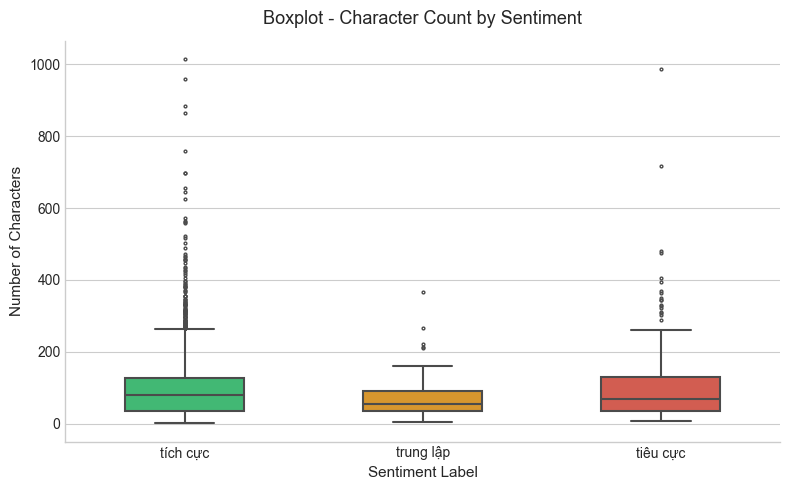
\includegraphics[width=0.9\textwidth]{graphics/boxplot_character_count_by_sentiment.png}
    \caption{Biểu đồ hộp số lượng ký tự theo nhãn cảm xúc.}
    \label{fig:boxplot_character_count_sentiment}
\end{figure}

Quan sát trực quan từ biểu đồ hộp của số lượng ký tự theo nhãn cảm xúc (Hình~\ref{fig:boxplot_character_count_sentiment}) cũng cho thấy khác biệt rõ ở phần đuôi phân phối. Mặc dù phần lớn bình luận của cả ba nhóm đều tập trung dưới ngưỡng 200 ký tự, nhóm tiêu cực có dải phân tán rộng hơn và xuất hiện nhiều ngoại lai ở vùng giá trị rất cao; một số mẫu vượt xa mốc 700 đến gần 1.000 ký tự. Ngược lại, nhóm trung lập có phân bố hẹp hơn, ít biến động và số lượng ngoại lai thấp hơn đáng kể, phản ánh xu hướng để lại nhận xét ngắn, trực tiếp và ít diễn giải.

\vspace{0.5em}
\noindent\textcolor{lightblue}{\textbf{Kiểm định Mann--Whitney U}}\par
\vspace{0.5em}
Để kiểm chứng một cách chặt chẽ giả thuyết rằng bình luận tiêu cực có xu hướng dài hơn bình luận tích cực, nhóm nghiên cứu áp dụng kiểm định phi tham số Mann--Whitney U trên phân phối số từ giữa hai nhóm. Việc lựa chọn kiểm định này là cần thiết vì phân phối độ dài văn bản bị lệch và không thỏa mãn giả định phân phối chuẩn. Kết quả thu được cho thấy thống kê kiểm định đạt $U = 538.779$, giá trị $p$ một phía bằng $0{,}032884$ và hệ số kích thước hiệu ứng đạt $r = 0{,}0271$. Đồng thời, trung vị số từ của nhóm tiêu cực là $15{,}0$, trong khi nhóm tích cực đạt $16{,}0$.

Với mức ý nghĩa $\alpha = 0{,}05$, giá trị $p < 0{,}05$ cho phép bác bỏ giả thuyết không, qua đó xác nhận rằng phân phối độ dài giữa hai nhóm có khác biệt về mặt thống kê. Tuy nhiên, cần nhấn mạnh rằng khác biệt này chủ yếu đến từ phần đuôi phân phối của nhóm tiêu cực --- nơi xuất hiện nhiều bình luận rất dài --- chứ không phản ánh sự chênh lệch lớn ở phần trung tâm của toàn bộ dữ liệu.

\vspace{0.5em}
\noindent\textcolor{lightblue}{\textbf{Kết luận thống kê}}\par
\vspace{0.5em}
Từ góc nhìn thực tiễn, mặc dù kiểm định cho kết quả có ý nghĩa thống kê, hệ số kích thước hiệu ứng $r = 0{,}0271$ là cực nhỏ và trung vị giữa hai nhóm gần như tương đương nhau. Điều này cho thấy đối với phần lớn bình luận thông thường, độ dài văn bản không tạo ra sự phân tách mạnh giữa cảm xúc tích cực và tiêu cực. Nói cách khác, đặc trưng độ dài chỉ mang tín hiệu bổ sung ở các trường hợp ngoại lệ, đặc biệt là những phản hồi tiêu cực có xu hướng mô tả dài và chi tiết hơn mức thông thường.

Do đó, \texttt{word\_count} và \texttt{char\_count} nên được xem là các đặc trưng phụ trợ thay vì đặc trưng quyết định. Khi kết hợp với các biểu diễn nội dung như TF-IDF hoặc vector ngữ nghĩa, nhóm đặc trưng này vẫn có giá trị trong việc bổ sung tín hiệu về cường độ diễn đạt, nhưng không đủ mạnh để sử dụng độc lập như nền tảng chính cho mô hình phân loại cảm xúc.

\subsubsection{Phân tích từ vựng}

\vspace{0.5em}
\noindent\textcolor{lightblue}{\textbf{Trực quan hóa đám mây từ vựng}}\par
\vspace{0.5em}
Trực quan hóa các từ vựng xuất hiện phổ biến nhất của các nhóm bình luận tích cực, trung lập và tiêu cực dưới dạng đám mây từ vựng giúp nhận diện nhanh những từ khóa trọng tâm cũng như khác biệt tổng quan về mặt ngữ nghĩa giữa các nhóm cảm xúc.

\begin{figure}[H]
    \centering
    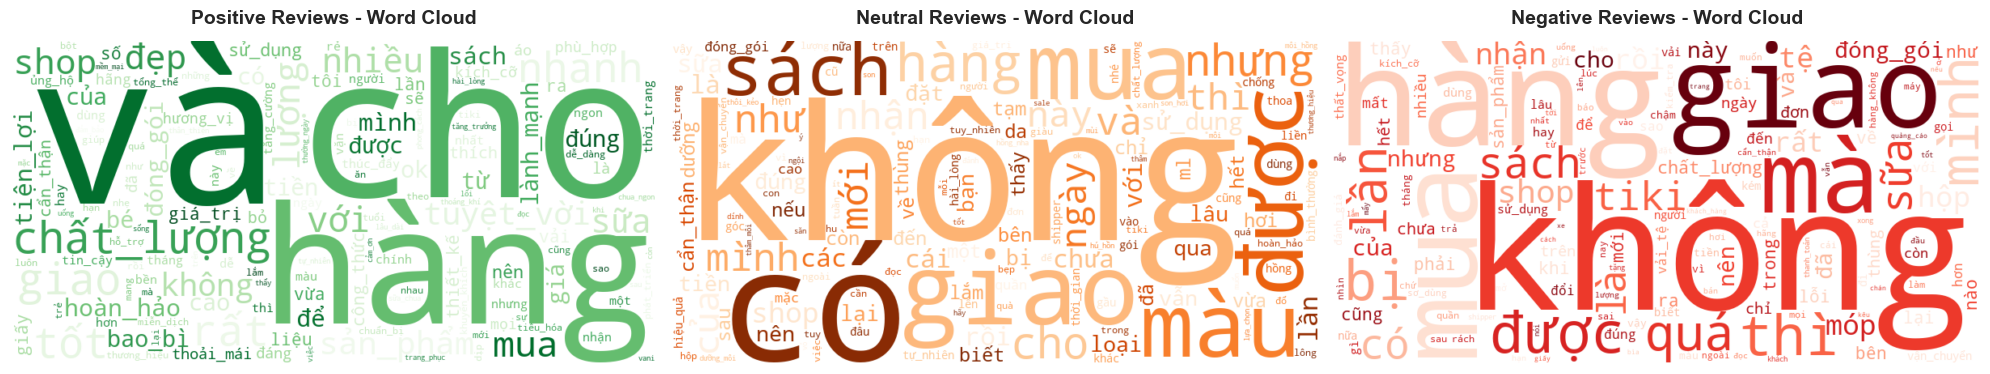
\includegraphics[width=\textwidth]{graphics/wordcloud_sentiment_groups.png}
    \caption{Đám mây từ vựng của ba nhóm cảm xúc: tích cực, trung lập và tiêu cực.}
    \label{fig:wordcloud_sentiment_groups}
\end{figure}

Nhận xét từ Hình~\ref{fig:wordcloud_sentiment_groups} có thể tóm lược như sau:

\begin{itemize}[labelsep=10pt, leftmargin=2cm]
    \item \textbf{Nhóm tích cực:} nổi bật với các từ khóa mang sắc thái khen ngợi rõ ràng như ``chất\_lượng'', ``tốt'', ``đẹp'', ``nhanh''. Điều này cho thấy người dùng chủ yếu bày tỏ sự hài lòng về chất lượng sản phẩm và tốc độ giao hàng.
    \item \textbf{Nhóm trung lập:} xuất hiện nhiều từ mang tính kể lể hoặc cấu trúc tương phản như ``nhưng'', ``không'', ``có''. Điều này cho thấy các đánh giá trung lập thường chứa cả yếu tố khen lẫn chê, phản ánh thái độ chấp nhận ở mức vừa phải.
    \item \textbf{Nhóm tiêu cực:} bị áp đảo bởi các từ chỉ sự cố và thái độ thất vọng như ``không'', ``bị'', ``tệ'', ``quá'', ``móp''. Khách hàng trong nhóm này tập trung phản ánh tình trạng hàng hóa lỗi hoặc trải nghiệm dịch vụ không đạt kỳ vọng.
\end{itemize}

\vspace{0.5em}
\noindent\textcolor{lightblue}{\textbf{Phân tích n-gram theo nhóm cảm xúc}}\par
\vspace{0.5em}
Phân tích top 20 unigram, bigram và trigram theo từng nhóm cảm xúc giúp bộc lộ các cụm từ đặc trưng mà phân tích đơn lẻ từng từ không thể nắm bắt được. Nhóm sử dụng \texttt{TfidfVectorizer} với \texttt{use\_idf=False} để đo tần suất thuần, tức chỉ xét tần suất xuất hiện của từ mà không điều chỉnh theo trọng số IDF.

\begin{figure}[H]
    \centering
    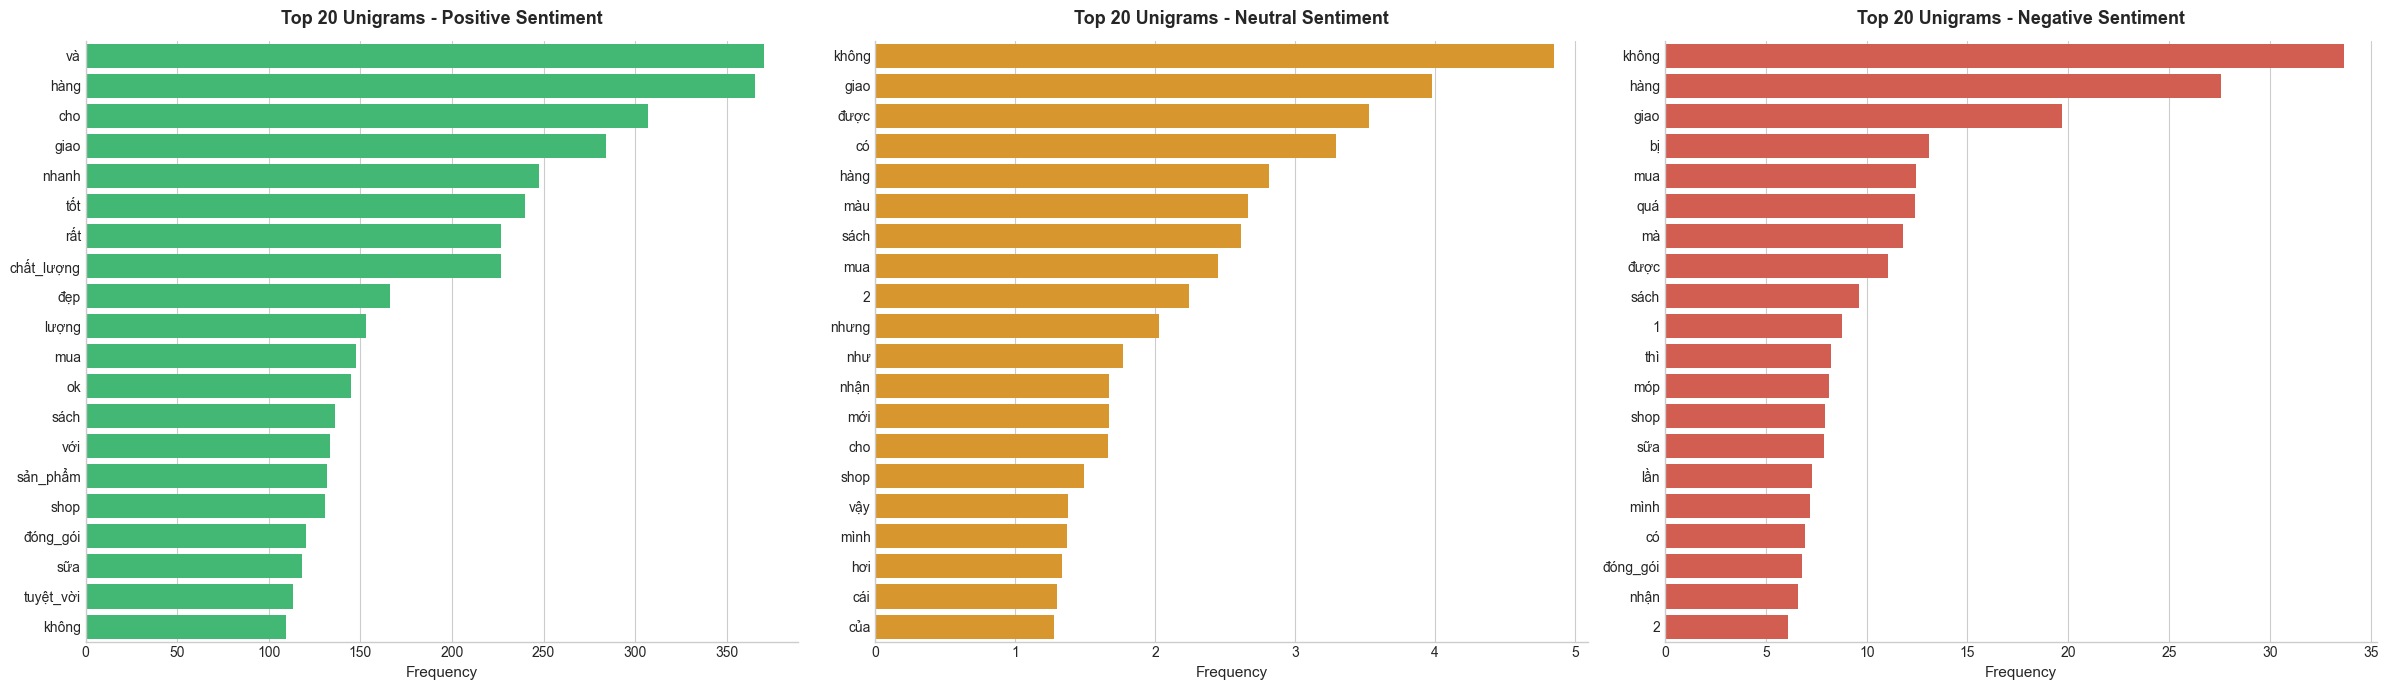
\includegraphics[width=\textwidth]{graphics/ngram_unigram_top20.png}
    \caption{Top 20 unigram theo ba nhóm cảm xúc: tích cực, trung lập và tiêu cực.}
    \label{fig:ngram_unigram_top20}
\end{figure}

\begin{figure}[H]
    \centering
    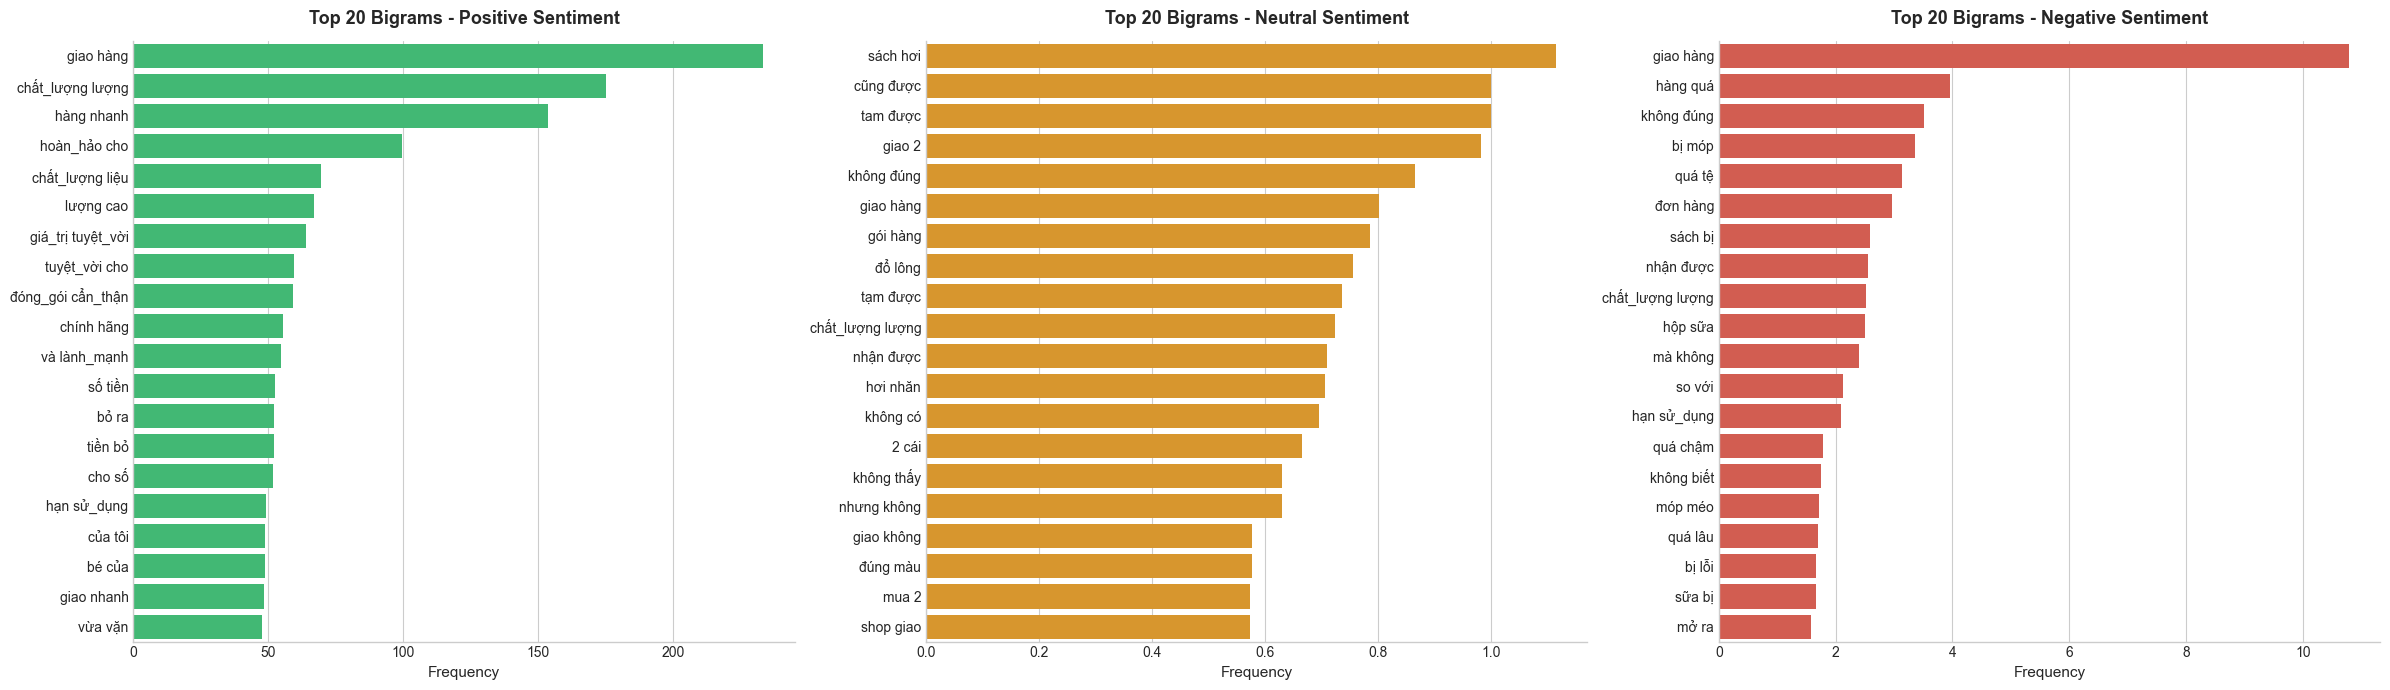
\includegraphics[width=\textwidth]{graphics/ngram_bigram_top20.png}
    \caption{Top 20 bigram theo ba nhóm cảm xúc: tích cực, trung lập và tiêu cực.}
    \label{fig:ngram_bigram_top20}
\end{figure}

\begin{figure}[H]
    \centering
    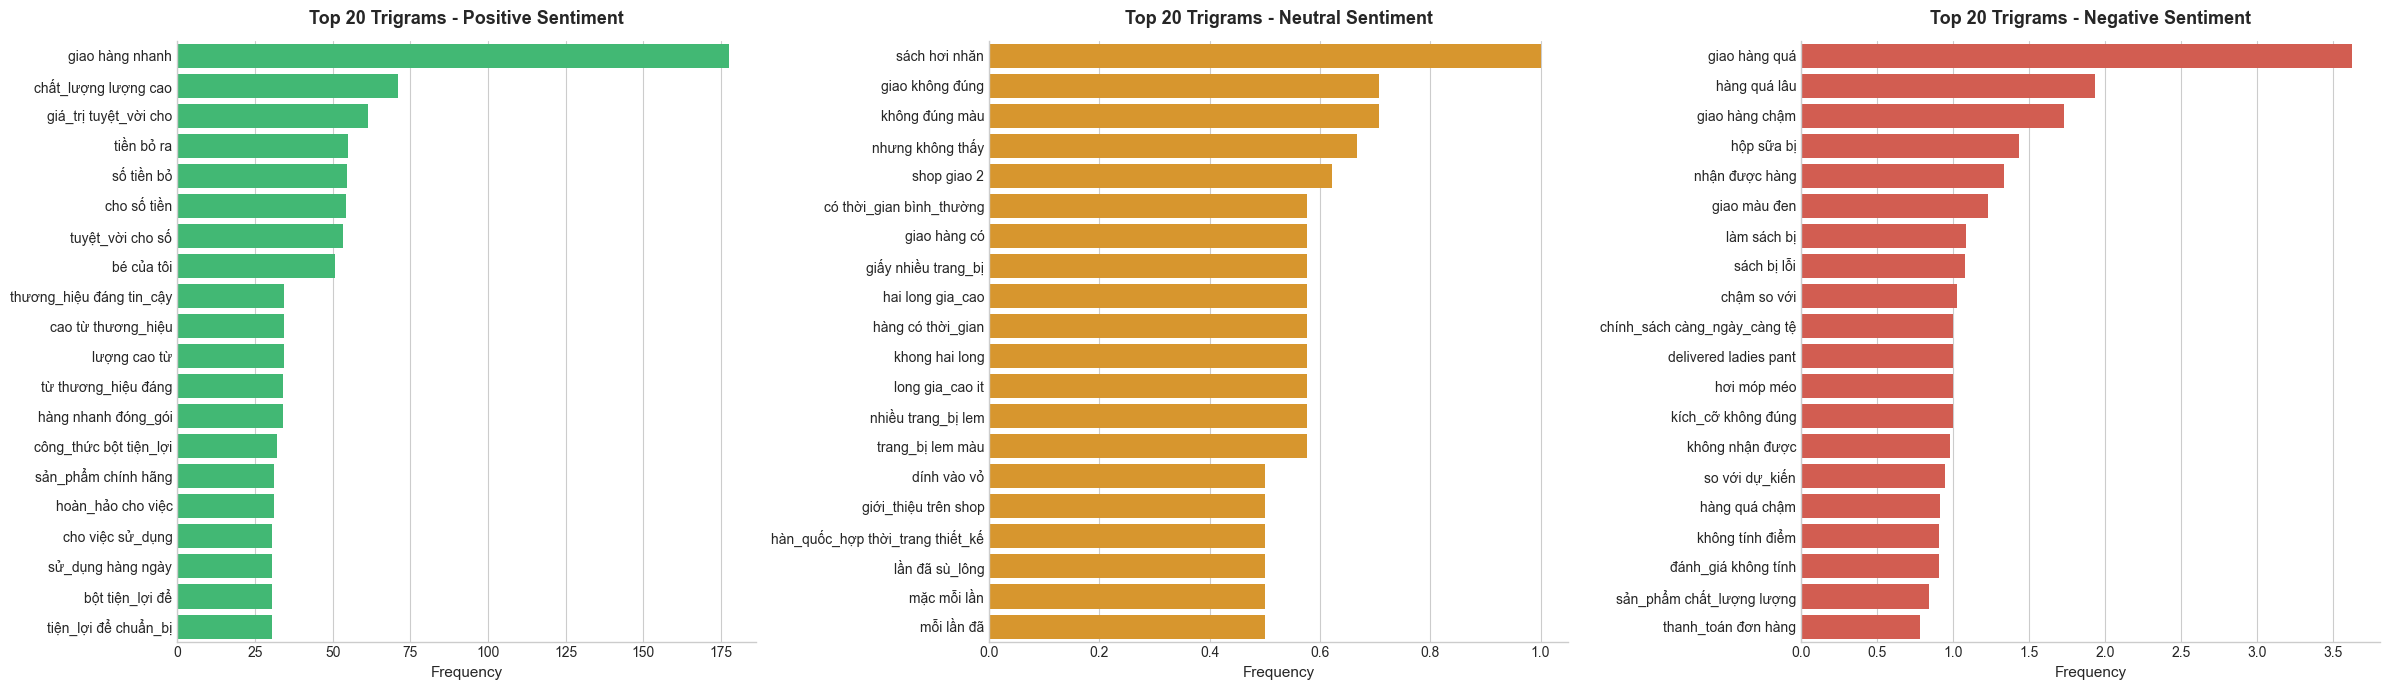
\includegraphics[width=\textwidth]{graphics/ngram_trigram_top20.png}
    \caption{Top 20 trigram theo ba nhóm cảm xúc: tích cực, trung lập và tiêu cực.}
    \label{fig:ngram_trigram_top20}
\end{figure}

Kết quả phân tích có thể được tóm lược như sau:

\begin{itemize}[labelsep=10pt, leftmargin=2cm]
    \item Ở cấp độ unigram, cả ba nhóm đều chứa các từ chung như ``hàng'' và ``giao'', do đó khả năng phân biệt sắc thái cảm xúc còn hạn chế.
    \item Khi chuyển sang bigram, ngữ cảnh đánh giá trở nên rõ ràng hơn đáng kể: nhóm tích cực thường gắn với các cụm như ``giao hàng nhanh'' và ``chất lượng tốt'', trong khi nhóm tiêu cực nổi bật với các biểu thức như ``giao hàng chậm'', ``bị móp'' hoặc ``không đúng''. Đối với nhóm trung lập, các cụm ``cũng được'' và ``tạm ổn'' phản ánh thái độ chấp nhận ở mức vừa phải.
    \item Ở cấp độ trigram, các tín hiệu ngữ nghĩa tiếp tục được củng cố. Những cụm như ``giao hàng quá lâu'' hoặc ``sách bị lỗi'' là các dấu hiệu phân biệt rất mạnh cho nhóm tiêu cực.
    \item Từ các quan sát trên, có thể kết luận rằng việc sử dụng cấu hình \texttt{ngram\_range=(1,\,2)} hoặc \texttt{(1,\,3)} trong bước vector hóa là cần thiết để thu thập được các tín hiệu ngôn ngữ phức hợp, thay vì chỉ dựa vào các từ đơn lẻ.
\end{itemize}

\vspace{0.5em}
\noindent\textcolor{lightblue}{\textbf{Tỷ lệ loại trên tổng số từ}}\par
\vspace{0.5em}
Tỷ lệ loại trên tổng số từ đo lường mức độ phong phú của từ vựng trong từng nhóm cảm xúc, được xác định bằng tỉ số giữa số lượng từ duy nhất và tổng số từ xuất hiện. Giá trị càng cao cho thấy ngôn ngữ càng đa dạng; ngược lại, giá trị thấp phản ánh xu hướng lặp lại khuôn mẫu diễn đạt.

\begin{center}
\renewcommand{\arraystretch}{1.4}
\begin{tabularx}{\textwidth}{|l|c|c|c|}
\hline
\rowcolor[HTML]{E8E8E8}
\textbf{Nhóm cảm xúc} & \textbf{Tổng số từ} & \textbf{Số từ duy nhất} & \textbf{Tỷ lệ loại trên tổng số từ} \\
\hline
Tích cực & $> 79.000$ & $\approx 4.400$ & $0{,}0560$ \\
\hline
Tiêu cực & $\approx 9.000$ & $\approx 1.900$ & $0{,}2076$ \\
\hline
Trung lập & $\approx 823$ & $\approx 385$ & $0{,}4678$ \\
\hline
\end{tabularx}
\captionof{table}{\centering Tỷ lệ loại trên tổng số từ theo nhóm cảm xúc}
\end{center}

Kết quả cho thấy nhóm tích cực có tỷ lệ thấp nhất dù quy mô dữ liệu lớn nhất, chứng tỏ các bình luận khen ngợi thường sử dụng một tập từ vựng khá lặp lại như ``tốt'', ``đẹp'', ``ok'', ``nhanh''. Ngược lại, nhóm tiêu cực có tỷ lệ cao hơn rõ rệt, phản ánh xu hướng dùng ngôn ngữ phong phú và chi tiết hơn để mô tả lỗi hoặc trải nghiệm không hài lòng. Đối với nhóm trung lập, giá trị cao nhất chủ yếu chịu ảnh hưởng bởi kích thước mẫu nhỏ; theo định luật Heap, tập dữ liệu càng nhỏ thì chỉ số này càng dễ tăng cao, do đó cần thận trọng khi diễn giải.

\vspace{0.5em}
\noindent\textcolor{lightblue}{\textbf{Kiểm chứng định luật Zipf}}\par
\vspace{0.5em}
Định luật Zipf phát biểu rằng tần suất của một từ tỷ lệ nghịch với thứ hạng của nó trên đồ thị log--log. Việc kiểm chứng quy luật này trên toàn bộ tập văn bản giúp đánh giá mức độ tự nhiên của ngôn ngữ và nhận diện vùng từ hiếm trước khi xây dựng ma trận đặc trưng.

\begin{figure}[H]
    \centering
    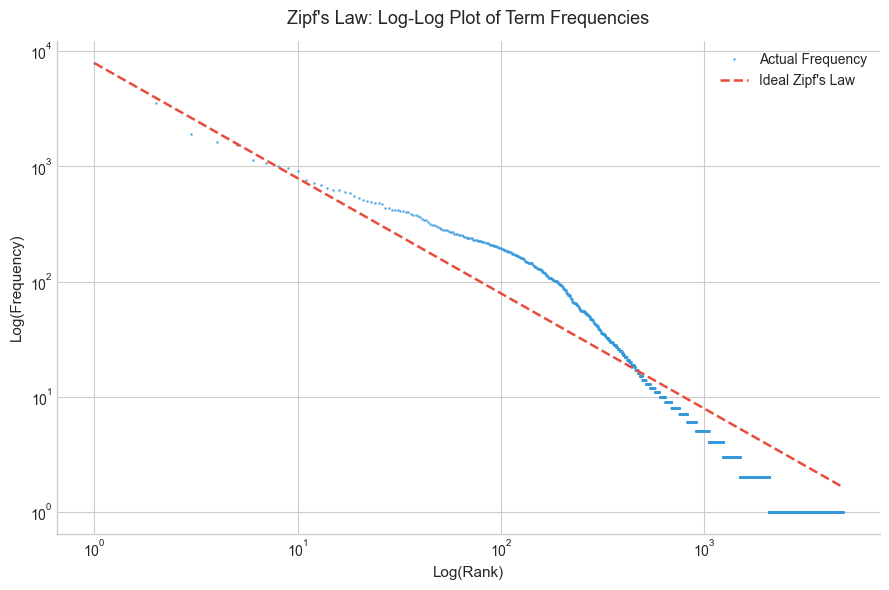
\includegraphics[width=0.9\textwidth]{graphics/zipf_kiem_chung.png}
    \caption{Kiểm chứng định luật Zipf trên tập văn bản đánh giá.}
    \label{fig:zipf_kiem_chung}
\end{figure}

Kết quả cho thấy đường quan sát bám khá sát đường Zipf lý tưởng ở phần đầu phân phối, xác nhận rằng tập dữ liệu tuân theo quy luật tự nhiên của ngôn ngữ con người và không bị chi phối bởi văn bản sinh ngẫu nhiên hay nhiễu bất thường. Ở dải thứ hạng từ 10 đến 100, đường quan sát nhô lên so với đường lý thuyết, phản ánh đặc điểm chuyên ngành của dữ liệu thương mại điện tử khi các từ như ``giao'', ``hàng'', ``chất lượng'' hay ``shop'' được lặp lại với tần suất cao hơn ngôn ngữ thông thường. Ở phần đuôi, đường cong giảm rất nhanh và tạo thành các bậc thang, cho thấy sự hiện diện của số lượng lớn từ hiếm chỉ xuất hiện một hoặc hai lần --- thường là lỗi chính tả, từ viết tắt bất thường hoặc tên sản phẩm đặc thù. Điều này củng cố sự cần thiết của việc thiết lập tham số \texttt{min\_df} trong bước vector hóa nhằm loại bỏ các từ quá hiếm và tránh làm ma trận TF-IDF phình to không cần thiết.

\subsubsection{Biểu diễn đặc trưng thưa --- TF-IDF}

Biểu diễn đặc trưng thưa bằng TF-IDF là một phương pháp kinh điển trong xử lý ngôn ngữ tự nhiên. Cách tiếp cận này biến đổi tập văn bản thành một không gian véc-tơ dựa trên tần suất xuất hiện tương đối của từ hoặc cụm từ n-gram, đồng thời làm giảm ảnh hưởng của các đơn vị ngôn ngữ xuất hiện quá phổ biến trong toàn bộ tập dữ liệu. Kết quả thu được là một ma trận dạng \texttt{(số tài liệu $\times$ số đặc trưng)} mà phần lớn các phần tử có giá trị bằng 0, qua đó phản ánh đúng bản chất thưa của dữ liệu văn bản sau vector hóa.

\vspace{0.5em}
\noindent\textcolor{lightblue}{\textbf{Vector hóa TF-IDF}}\par
\vspace{0.5em}
Ở bước này, nhóm nghiên cứu khởi tạo và huấn luyện bộ biến đổi TF-IDF để chuyển tập đánh giá thành ma trận đặc trưng thưa. Quá trình này đồng thời kiểm soát số chiều của không gian biểu diễn và loại bỏ các từ quá hiếm thông qua các tham số như \texttt{min\_df} và \texttt{max\_features}, nhằm cân bằng giữa khả năng biểu diễn nội dung và chi phí tính toán.

\begin{center}
\renewcommand{\arraystretch}{1.4}
\begin{tabularx}{0.75\textwidth}{|X|c|}
\hline
\rowcolor[HTML]{E8E8E8}
\textbf{Thuộc tính} & \textbf{Giá trị} \\
\hline
Kích thước ma trận (tài liệu $\times$ đặc trưng) & $4.651 \times 4.408$ \\
\hline
Số phần tử khác 0 & $102.320$ \\
\hline
Tỷ lệ thưa thớt & $99,50\%$ \\
\hline
Bộ nhớ sử dụng & $0,82$ MB \\
\hline
\end{tabularx}
\captionof{table}{\centering Các thuộc tính chính của ma trận TF-IDF}
\end{center}

Các thông số trên cho thấy ma trận đặc trưng sau vector hóa có mức độ thưa thớt rất cao, với chỉ khoảng $0,5\%$ số phần tử khác 0. Đây là đặc điểm điển hình của biểu diễn TF-IDF trên dữ liệu đánh giá ngắn, nơi mỗi văn bản chỉ kích hoạt một tập nhỏ đặc trưng trong toàn bộ từ vựng. Dung lượng bộ nhớ chỉ ở mức $0,82$ MB cho thấy biểu diễn này vẫn khá gọn nhẹ, phù hợp cho các mô hình học máy tuyến tính và các bước phân tích không gian đặc trưng tiếp theo.

\vspace{0.5em}
\noindent\textcolor{lightblue}{\textbf{Trực quan hóa t-SNE}}\par
\vspace{0.5em}
Nhóm nghiên cứu tiếp tục áp dụng thuật toán giảm chiều t-SNE để chiếu không gian TF-IDF xuống mặt phẳng hai chiều. Bước này giúp trực quan hóa hình học của không gian đặc trưng và đánh giá xem các nhóm cảm xúc có thực sự phân tách thành các cụm riêng biệt hay không.

\begin{figure}[H]
    \centering
    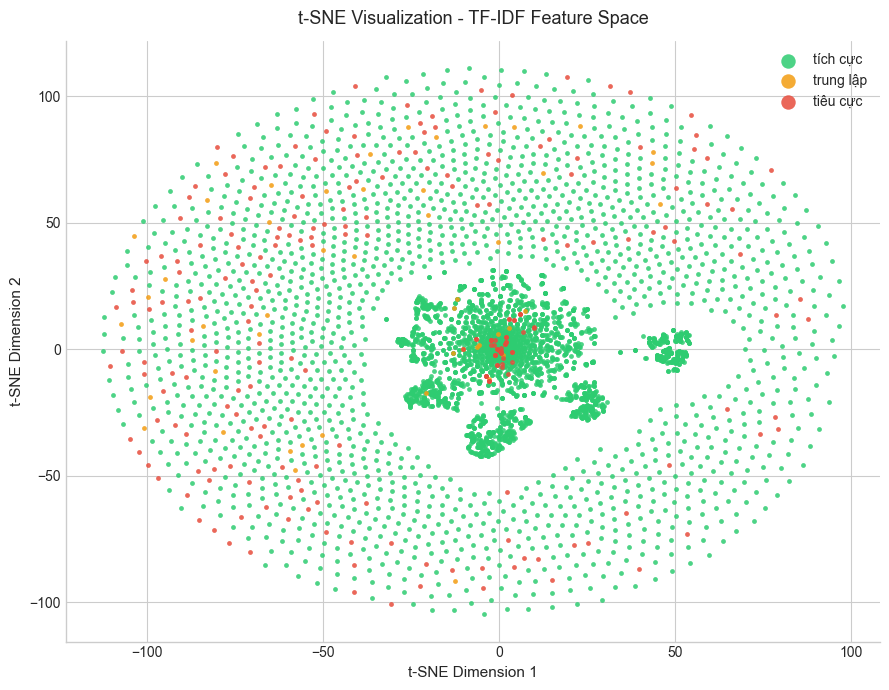
\includegraphics[width=0.92\textwidth]{graphics/tsne_tfidf_feature_space.png}
    \caption{Trực quan hóa t-SNE không gian đặc trưng TF-IDF theo ba nhóm cảm xúc.}
    \label{fig:tsne_tfidf_feature_space}
\end{figure}

Nhận xét từ biểu đồ t-SNE trong Hình~\ref{fig:tsne_tfidf_feature_space} có thể được tóm lược như sau:

\begin{itemize}[labelsep=10pt, leftmargin=2cm]
    \item \textbf{Bị chi phối bởi dữ liệu mất cân bằng:} lớp tích cực chiếm số lượng áp đảo và phủ gần như toàn bộ không gian phân phối. Điều này phản ánh đúng tình trạng mất cân bằng nhãn của tập dữ liệu gốc, trong đó phần lớn đánh giá thuộc nhóm tích cực.
    \item \textbf{Ranh giới phân loại chồng lấp mạnh:} các điểm tiêu cực và trung lập phân tán rải rác, đồng thời trộn lẫn đáng kể vào đám mây điểm tích cực. Chúng không hình thành các cụm độc lập, tách biệt rõ ràng trong không gian hai chiều.
    \item \textbf{Hạn chế của biểu diễn TF-IDF:} sự chồng lấp trên cho thấy TF-IDF chủ yếu gom nhóm dựa trên sự xuất hiện của các từ vựng bề mặt phổ biến như ``hàng'', ``giao'', ``shop'' mà chưa đủ khả năng tách bạch các sắc thái ngữ nghĩa sâu hơn. Điều này dự báo rằng các mô hình phân loại tuyến tính cơ bản sẽ gặp khó khăn khi phải xác định ranh giới quyết định chính xác, đặc biệt đối với các lớp thiểu số.
\end{itemize}

\subsubsection{Biểu diễn ngữ nghĩa dày đặc --- Vietnamese SBERT}

Trái ngược với biểu diễn TF-IDF vốn chủ yếu dựa trên tần suất bề mặt của từ vựng, biểu diễn ngữ nghĩa dày đặc hướng tới việc bảo toàn ngữ nghĩa sâu của câu thông qua các mô hình biến áp câu. Trong nghiên cứu này, nhóm sử dụng mô hình \texttt{keepitreal/vietnamese-sbert} để mã hóa mỗi bình luận thành một véc-tơ có số chiều cố định nhưng chứa hàm lượng thông tin ngữ nghĩa cao. Trong không gian này, các câu có ý nghĩa tương đồng có xu hướng nằm gần nhau về mặt hình học, ngay cả khi chúng không chia sẻ cùng từ vựng bề mặt.

\vspace{0.5em}
\noindent\textcolor{lightblue}{\textbf{Mã hóa bằng Vietnamese SBERT}}\par
\vspace{0.5em}
Nhóm nghiên cứu sử dụng mô hình SBERT chuyên biệt cho tiếng Việt để chuyển đổi toàn bộ tập bình luận thành các véc-tơ nhúng dày đặc. Khác với TF-IDF chỉ đếm số lần xuất hiện của từ khóa, SBERT có khả năng nắm bắt ngữ cảnh và mức độ tương đồng ngữ nghĩa giữa các câu, kể cả trong trường hợp cách diễn đạt khác nhau nhưng nội dung tương đương.

\begin{center}
\renewcommand{\arraystretch}{1.4}
\begin{tabularx}{0.7\textwidth}{|X|c|}
\hline
\rowcolor[HTML]{E8E8E8}
\textbf{Thuộc tính} & \textbf{Giá trị} \\
\hline
Kích thước ma trận nhúng dày đặc & $(4.651,\ 768)$ \\
\hline
Số tài liệu $\times$ số chiều & $4.651 \times 768$ \\
\hline
Bộ nhớ sử dụng & $14,3$ MB \\
\hline
\end{tabularx}
\captionof{table}{\centering Các thuộc tính chính của ma trận nhúng ngữ nghĩa dày đặc}
\end{center}

Kích thước ma trận cho thấy mỗi bình luận được ánh xạ vào một véc-tơ 768 chiều, tạo thành không gian đặc trưng dày đặc có khả năng biểu diễn nội dung ở mức ngữ nghĩa thay vì chỉ ở mức từ vựng rời rạc. Mặc dù dung lượng bộ nhớ tăng lên so với biểu diễn TF-IDF, chi phí này đổi lại khả năng mã hóa tốt hơn các quan hệ ngữ nghĩa giữa các câu, từ đó mở ra tiềm năng phân tách lớp hiệu quả hơn trong các bước trực quan hóa và mô hình hóa tiếp theo.

\vspace{0.5em}
\noindent\textcolor{lightblue}{\textbf{Trực quan hóa t-SNE trên không gian dày đặc}}\par
\vspace{0.5em}
Sau khi thu được ma trận nhúng ngữ nghĩa, nhóm tiếp tục áp dụng thuật toán t-SNE để giảm chiều không gian dày đặc xuống hai chiều nhằm phục vụ trực quan hóa. Việc đối chiếu biểu đồ này với biểu đồ t-SNE của TF-IDF sẽ giúp đánh giá liệu biểu diễn SBERT có thực sự kéo các bình luận cùng sắc thái cảm xúc lại gần nhau hơn và tách các nhóm tốt hơn hay không.

\begin{figure}[H]
    \centering
    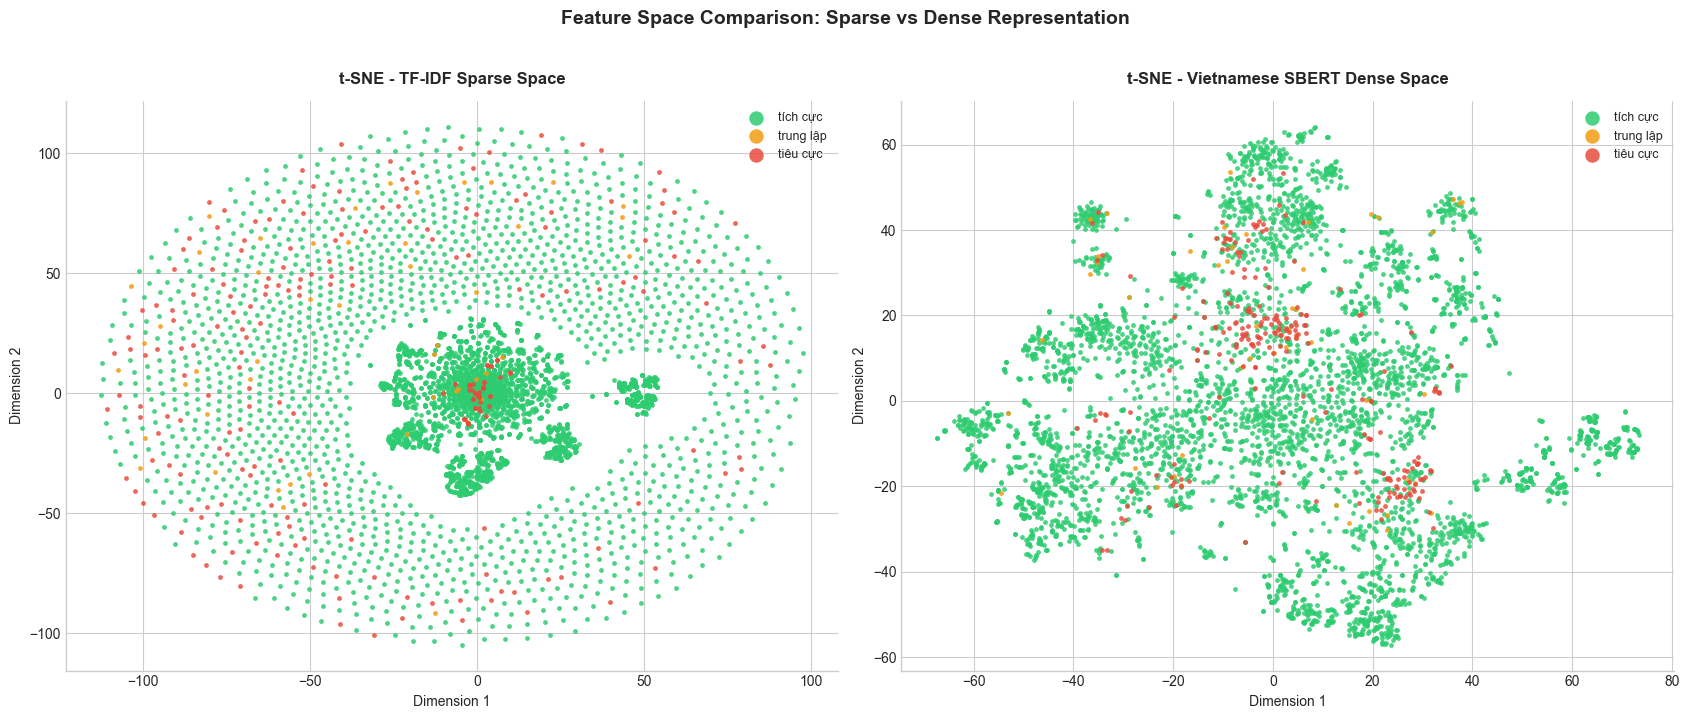
\includegraphics[width=\textwidth]{graphics/compare_tfidf_sbert_tsne.png}
    \caption{So sánh trực quan không gian đặc trưng TF-IDF và Vietnamese SBERT sau khi giảm chiều bằng t-SNE.}
    \label{fig:compare_tfidf_sbert_tsne}
\end{figure}

Nhận xét khi so sánh hai không gian đặc trưng trong Hình~\ref{fig:compare_tfidf_sbert_tsne} có thể được tóm lược như sau:

\begin{itemize}[labelsep=10pt, leftmargin=2cm]
    \item \textbf{Hình thái phân bố:} biểu đồ TF-IDF tạo ra một cấu trúc hình khuyên khá nhân tạo với lõi đặc và viền thưa, vốn là một dạng hiện tượng thường gặp khi áp dụng t-SNE trên dữ liệu quá thưa. Ngược lại, không gian SBERT phân bố tự nhiên và hữu cơ hơn, hình thành nhiều cụm nhỏ mang ý nghĩa ngữ nghĩa rõ ràng hơn.
    \item \textbf{Khả năng gom nhóm:} trong không gian TF-IDF, các điểm tiêu cực và trung lập rải rác khá ngẫu nhiên và bị hòa lẫn mạnh vào lớp tích cực. Khi chuyển sang không gian dày đặc của SBERT, các điểm tiêu cực bắt đầu có xu hướng co cụm tại một số vùng cục bộ, cho thấy biểu diễn ngữ nghĩa đã giữ lại được tín hiệu cấu trúc tốt hơn.
    \item \textbf{Kết luận trực quan:} mặc dù hiện tượng chồng lấp vẫn tồn tại do tập dữ liệu mất cân bằng nặng, biểu đồ cho thấy SBERT đã nắm bắt tốt hơn các tương đồng ngữ nghĩa sâu xa và kéo các bình luận có nội dung gần nhau lại gần hơn so với phương pháp đếm từ khóa bề mặt như TF-IDF.
\end{itemize}

\subsubsection{Thử nghiệm gom cụm K-Means không giám sát}

Nhóm nghiên cứu tiến hành thử nghiệm thuật toán gom cụm K-Means với số cụm $k=3$ trên không gian nhúng ngữ nghĩa của SBERT mà không sử dụng trước nhãn cảm xúc. Mục tiêu của phép thử này là đánh giá xem cấu trúc hình học của không gian SBERT có đủ mạch lạc để tự hình thành các cụm tự nhiên hay không, từ đó cung cấp thêm bằng chứng về chất lượng biểu diễn ngữ nghĩa dày đặc.

\begin{figure}[H]
    \centering
    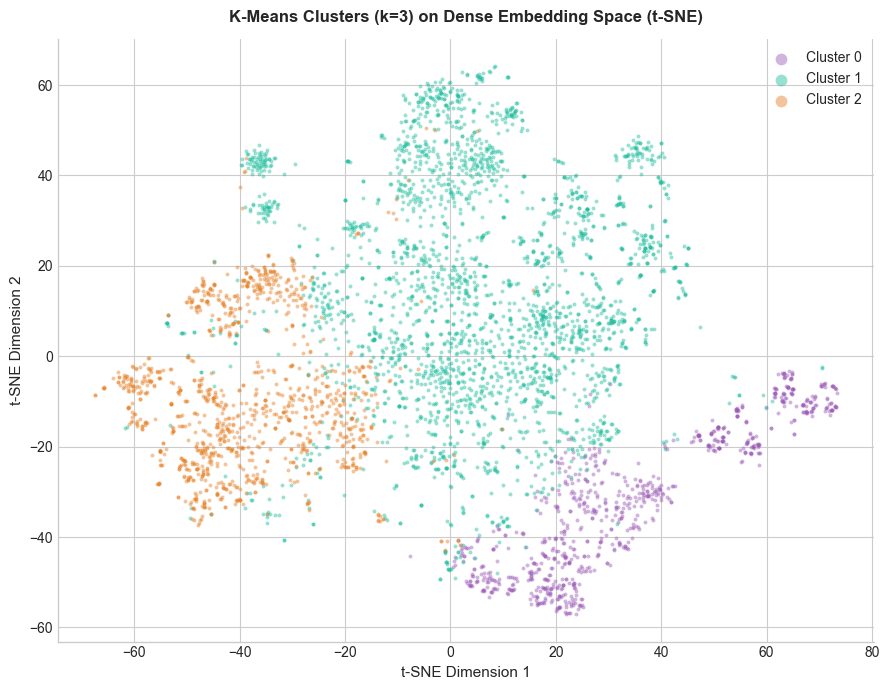
\includegraphics[width=0.92\textwidth]{graphics/kmeans_sbert_tsne.png}
    \caption{Các cụm K-Means $(k=3)$ trên không gian nhúng SBERT sau khi giảm chiều bằng t-SNE.}
    \label{fig:kmeans_sbert_tsne}
\end{figure}

Nhận xét từ kết quả gom cụm trong Hình~\ref{fig:kmeans_sbert_tsne} có thể được tóm lược như sau:

\begin{itemize}[labelsep=10pt, leftmargin=2cm]
    \item \textbf{Phân cụm rõ nét:} dù không được cung cấp nhãn cảm xúc từ trước, thuật toán K-Means vẫn tự động chia không gian SBERT thành ba cụm hình học tương đối tách biệt. Điều này cho thấy không gian đặc trưng dày đặc sở hữu cấu trúc toán học đủ ổn định để hỗ trợ các phương pháp học không giám sát.
    \item \textbf{Gom cụm theo chủ đề ngữ nghĩa:} do dữ liệu tích cực chiếm tỷ trọng áp đảo, ba cụm thu được không nhất thiết tương ứng hoàn toàn với ba nhãn cảm xúc, mà nhiều khả năng phản ánh ba chủ đề ngữ nghĩa tự nhiên trong đánh giá của khách hàng, chẳng hạn như khen giao hàng, khen sản phẩm hoặc phản ánh vấn đề phát sinh.
    \item \textbf{Ưu thế của SBERT:} kết quả trực quan này củng cố nhận định rằng SBERT vượt trội hơn TF-IDF trong việc nắm bắt quan hệ ngữ nghĩa sâu. Nhờ đó, biểu diễn này đặc biệt phù hợp làm đầu vào cho các mô hình học sâu hoặc các chiến lược học biểu diễn nâng cao ở giai đoạn tiếp theo.
\end{itemize}

\subsection{Khám phá chuyên sâu đặc trưng dữ liệu hình ảnh ngoại tuyến}
% Nội dung đồng đội cần viết:
% - Thống kê chất lượng hình ảnh: trực quan hóa phân bố độ phân giải và giá trị phân bố điểm ảnh của tập dữ liệu thị giác.
% - Phân tích đặc tính thị giác: khảo sát độ sáng tối trung bình và độ tương phản giữa các nhóm nhãn hình ảnh khác nhau nhằm nhận diện ngoại lệ (ảnh quá mờ hoặc lóa).
% - Kiểm tra chất lượng nâng cao: ứng dụng thuật toán băm cảm nhận để quét và định lượng tỷ lệ trùng lặp hình ảnh, phát hiện các trường hợp mượn ảnh từ nguồn khác để đánh giá.
\label{sec:phan_tich_du_lieu_anh}

Phần này trình bày kết quả phân tích khám phá đối với tập ảnh sau bước kiểm
tra chất lượng (Mục~\ref{sec:kiem_tra_du_lieu_anh}), tập trung vào bốn khía
cạnh: phân bố độ phân giải gốc, phân phối cường độ điểm ảnh theo kênh màu,
đặc trưng quang học theo nhãn kết hợp nhận diện ngoại lệ, và phân tích chuyên
sâu về trùng lặp ảnh nhằm phát hiện khả năng gán nhãn sai liên nhãn.

% ─────────────────────────────────────────────────────────────────────────────
\paragraph{Phân bố độ phân giải.}
Quét toàn bộ 7.987 ảnh ở kích thước gốc (không áp dụng resize) cho kết quả
thống kê mô tả được trình bày tại Bảng~\ref{tab:resolution_stats} và trực quan
hóa tại Hình~\ref{fig:resolution_distribution}.

\begin{table}[H]
    \centering
    \caption{Thống kê mô tả độ phân giải gốc của tập dữ liệu hình ảnh}
    \label{tab:resolution_stats}
    \begin{tabular}{lrrr}
        \hline
        \textbf{Chỉ số} & \textbf{Chiều rộng (px)} & \textbf{Chiều cao (px)}
            & \textbf{Tỉ lệ khung hình} \\
        \hline
        Trung bình  &   975,6 & 1.256,1 & 0,8 \\
        Độ lệch chuẩn & 931,5 &   967,3 & 0,4 \\
        Nhỏ nhất    &    85,0 &    51,0 & 0,3 \\
        Phân vị 25  &   360,0 &   640,0 & 0,6 \\
        Trung vị    &   692,0 &   834,0 & 0,7 \\
        Phân vị 75  & 1.080,0 & 1.440,0 & 0,8 \\
        Lớn nhất    & 5.760,0 & 5.712,0 & 6,1 \\
        \hline
    \end{tabular}
\end{table}

\begin{figure}[H]
    \centering
    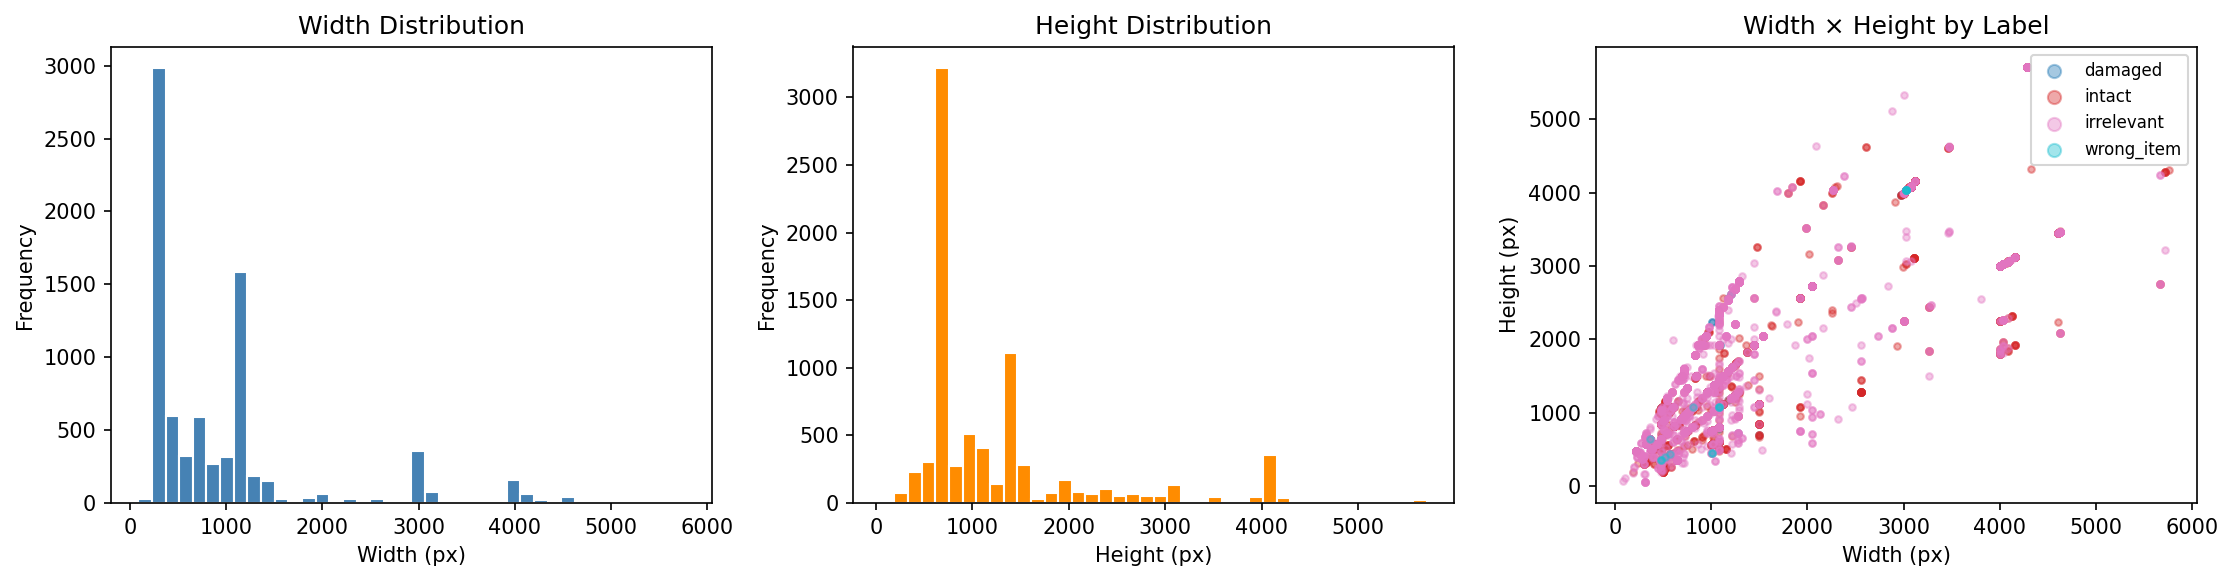
\includegraphics[width=\textwidth]{graphics/resolution_distribution.png}
    \caption{Phân bố chiều rộng, chiều cao và tương quan Width$\times$Height
        theo nhãn của toàn bộ tập dữ liệu.}
    \label{fig:resolution_distribution}
\end{figure}

Phân bố chiều rộng biểu hiện dạng lưỡng đỉnh với cực đại đầu tiên tập trung
quanh 360\,px và cực đại thứ hai quanh 1.080\,px, phản ánh sự tồn tại của hai
nhóm ảnh có nguồn gốc thu thập khác nhau. Phân bố chiều cao tập trung mạnh
quanh 960\,px nhưng có đuôi phải kéo dài đến hơn 5.000\,px, cho thấy một số
ảnh dọc có tỉ lệ khung hình đặc biệt. Biểu đồ tán xạ Width$\times$Height cho
thấy phần lớn mẫu thuộc nhãn \texttt{irrelevant} nằm rải rác trên toàn không
gian độ phân giải, trong khi các nhãn \texttt{damaged} và \texttt{intact} có xu
hướng tập trung hơn. Tổng số ảnh dưới ngưỡng 64$\times$64\,px là 6 mẫu
(0,08\%), toàn bộ thuộc nhãn \texttt{irrelevant}, xác nhận rằng mức độ ảnh có
độ phân giải quá thấp là không đáng kể trong tập dữ liệu.

Độ phân giải trung vị đạt 692$\times$834\,px với tỉ lệ khung hình trung vị 0,7
(ảnh dọc), biện hộ cho ngưỡng resize tối thiểu $64\times64$\,px đã được xác lập
trong bước kiểm tra chất lượng (Mục~\ref{sec:kiem_tra_du_lieu_anh}) và kích
thước làm việc $128\times128$\,px được chọn cho các phân tích nặng.

% ─────────────────────────────────────────────────────────────────────────────
\paragraph{Phân phối cường độ điểm ảnh.}
Phân tích phân phối cường độ điểm ảnh theo từng kênh màu trên tập mẫu 518 ảnh
(Hình~\ref{fig:pixel_distribution}) cho thấy cả ba kênh R, G, B đều biểu hiện
phân phối lưỡng đỉnh: cực đại thứ nhất tập trung ở vùng cường độ thấp (lân cận
0) và cực đại thứ hai nằm trong khoảng cường độ trung bình đến cao
(100\textendash 180). Cấu trúc phân phối này phản ánh sự tồn tại đồng thời của
hai nhóm ảnh có điều kiện chiếu sáng đối lập trong tập dữ liệu và xác nhận sự
cần thiết của bước chuẩn hóa cường độ điểm ảnh trước khi đưa dữ liệu vào mô
hình.

\begin{figure}[H]
    \centering
    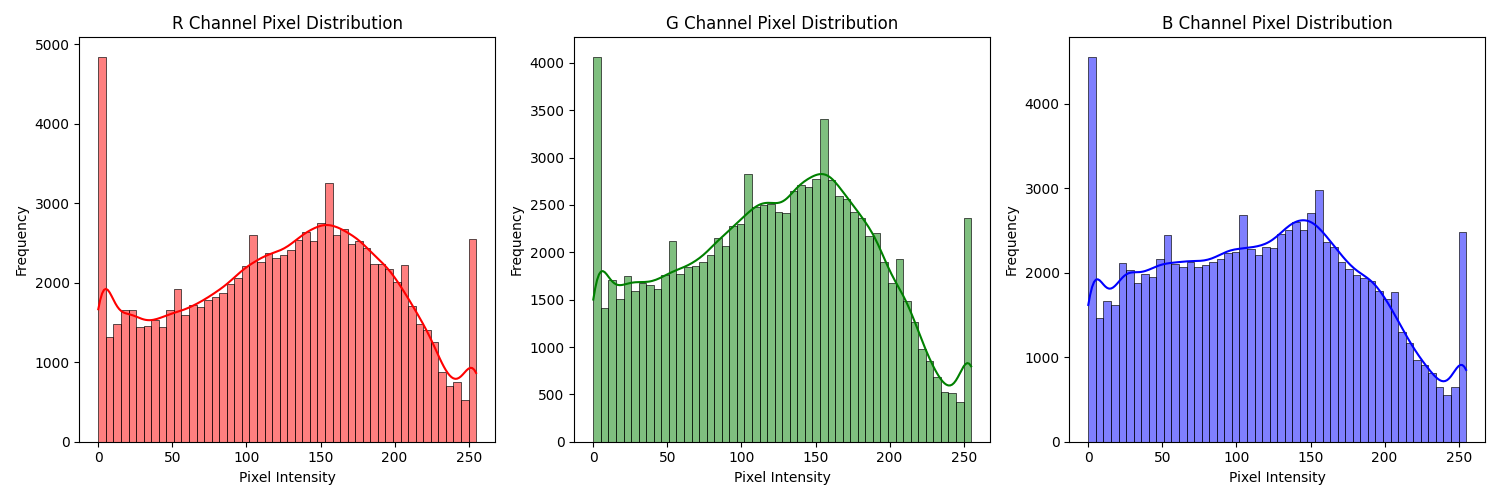
\includegraphics[width=\textwidth]{graphics/pixel_distribution.png}
    \caption{Phân phối cường độ điểm ảnh theo ba kênh màu R, G, B trên tập
        mẫu 518 ảnh.}
    \label{fig:pixel_distribution}
\end{figure}

% ─────────────────────────────────────────────────────────────────────────────
\paragraph{Đặc trưng quang học theo nhãn và nhận diện ngoại lệ.}
Cường độ sáng trung bình và độ tương phản --- đo bằng độ lệch chuẩn cường độ
trên ảnh thang xám --- được tổng hợp theo nhãn tại
Bảng~\ref{tab:brightness_contrast} và Hình~\ref{fig:brightness_contrast}.

\begin{table}[H]
    \centering
    \caption{Cường độ sáng trung bình và độ tương phản theo nhãn}
    \label{tab:brightness_contrast}
    \begin{tabular}{lcc}
        \hline
        \textbf{Nhãn} & \textbf{Cường độ sáng trung bình}
            & \textbf{Độ tương phản (độ lệch chuẩn)} \\
        \hline
        \texttt{damaged}     & 127,87 & 53,38 \\
        \texttt{intact}      & 123,03 & 51,36 \\
        \texttt{irrelevant}  & 116,92 & 45,60 \\
        \texttt{wrong\_item} & 107,30 & 53,58 \\
        \hline
    \end{tabular}
\end{table}

\begin{figure}[H]
    \centering
    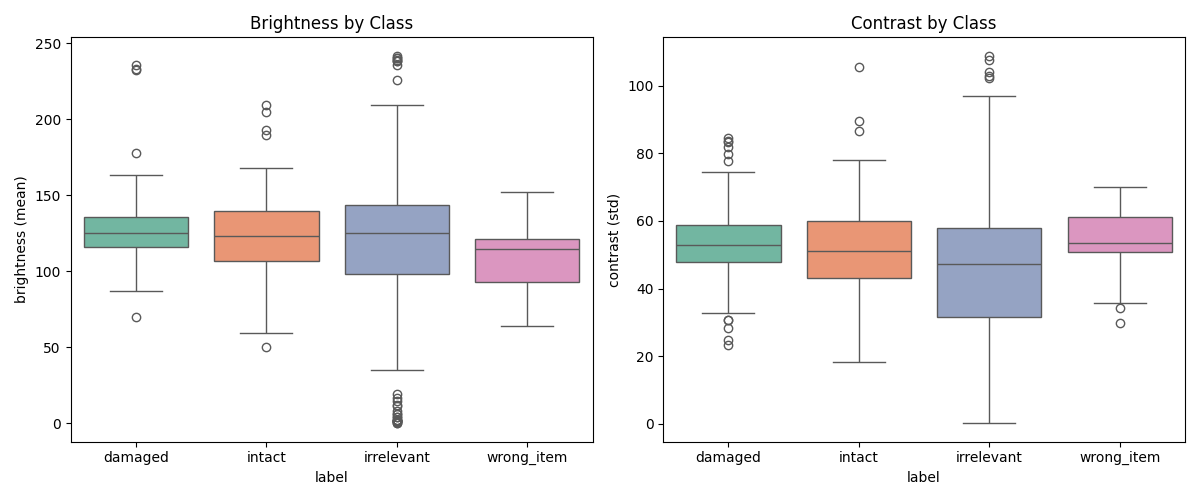
\includegraphics[width=\textwidth]{graphics/brightness_contrast_boxplot.png}
    \caption{Phân bố cường độ sáng và độ tương phản theo nhãn (biểu đồ hộp).}
    \label{fig:brightness_contrast}
\end{figure}

Nhãn \texttt{damaged} ghi nhận cường độ sáng trung bình cao nhất (127,87),
trong khi nhãn \texttt{wrong\_item} có giá trị thấp nhất (107,30). Nhãn
\texttt{irrelevant} có độ tương phản thấp nhất (45,60), phản ánh đặc tính cấu
trúc ảnh đồng nhất hơn so với các nhãn còn lại --- phù hợp với bản chất của
các ảnh không liên quan đến đối tượng sản phẩm cần phân loại.

Áp dụng ngưỡng phát hiện ngoại lệ (cường độ sáng $<50$ hoặc $>200$; độ tương
phản $<20$) trên tập mẫu 518 ảnh phát hiện 49 ảnh ngoại lệ, chiếm 9,5\% tập
mẫu. Bảng~\ref{tab:outlier_summary} trình bày phân bố ngoại lệ theo nhãn và
loại lỗi.

\begin{table}[H]
    \centering
    \caption{Phân bố ảnh ngoại lệ theo nhãn và loại lỗi quang học}
    \label{tab:outlier_summary}
    \begin{tabular}{llc}
        \hline
        \textbf{Nhãn} & \textbf{Loại ngoại lệ} & \textbf{Số lượng} \\
        \hline
        \texttt{damaged}    & Quá sáng (\textit{overexposed})              &  3 \\
        \texttt{intact}     & Độ tương phản thấp (\textit{low\_contrast})  &  1 \\
        \texttt{intact}     & Quá sáng (\textit{overexposed})              &  2 \\
        \texttt{intact}     & Quá tối (\textit{too\_dark})                 &  1 \\
        \texttt{irrelevant} & Độ tương phản thấp (\textit{low\_contrast})  &  3 \\
        \texttt{irrelevant} & Quá sáng (\textit{overexposed})              & 10 \\
        \texttt{irrelevant} & Quá tối (\textit{too\_dark})                 & 10 \\
        \texttt{irrelevant} & Quá tối + Độ tương phản thấp                & 19 \\
        \hline
        \textbf{Tổng}       &                                              & \textbf{49} \\
        \hline
    \end{tabular}
\end{table}

Nhãn \texttt{irrelevant} chiếm ưu thế tuyệt đối với 42/49 trường hợp ngoại lệ,
trong đó nhóm ảnh vừa quá tối vừa có độ tương phản thấp (19 mẫu) đặc trưng cho
các ảnh gần như hoàn toàn đen --- nhiều khả năng là ảnh lỗi từ thiết bị thu
thập. Các ngoại lệ này không bị loại bỏ tự động nhưng được lưu vào tệp
\texttt{outlier\_report.csv} để phục vụ rà soát thủ công, đặc biệt đối với
nhãn \texttt{damaged} nhằm tránh làm giảm chất lượng tín hiệu học của nhãn
thiểu số.

% ─────────────────────────────────────────────────────────────────────────────
\paragraph{Phân tích chuyên sâu trùng lặp ảnh.}
Kết quả quét pHash (Mục~\ref{sec:kiem_tra_du_lieu_anh}) cho thấy 2.984 cặp ảnh
gần trùng. Phân tích chuyên sâu phân loại các cặp này theo quan hệ nhãn
(Hình~\ref{fig:duplicate_analysis}) và trình bày tại
Bảng~\ref{tab:duplicate_summary}.

\begin{table}[H]
    \centering
    \caption{Phân loại cặp ảnh trùng lặp theo quan hệ nhãn}
    \label{tab:duplicate_summary}
    \begin{tabular}{lcc}
        \hline
        \textbf{Phân loại} & \textbf{Số cặp} & \textbf{Tỉ trọng (\%)} \\
        \hline
        Trùng lặp cùng nhãn (\textit{intra-class}) & 2.894 & 96,98 \\
        Trùng lặp khác nhãn (\textit{cross-class}) &    90 &  3,02 \\
        \quad Trong đó: trùng chính xác (khoảng cách Hamming = 0) & 46 & 1,54 \\
        \hline
        \textbf{Tổng}      & 2.984 & 100,00 \\
        \hline
    \end{tabular}
\end{table}

\begin{figure}[H]
    \centering
    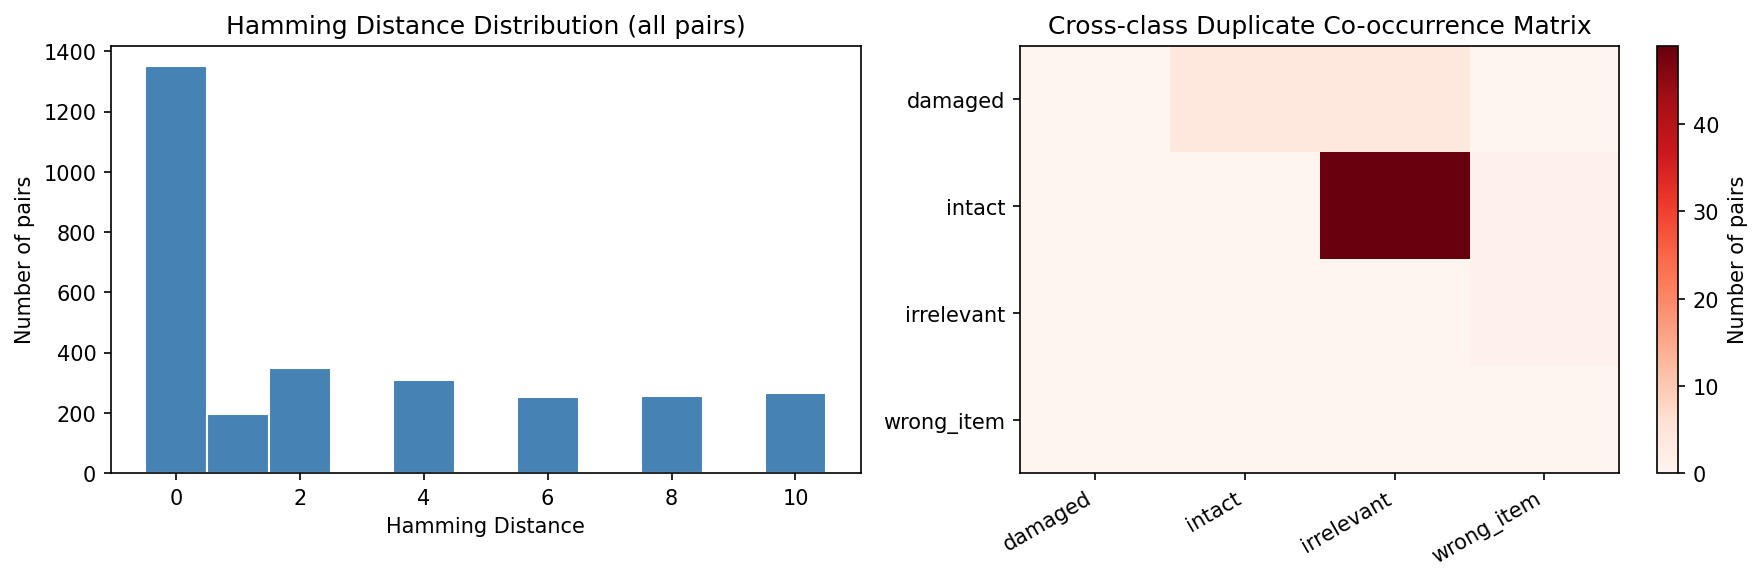
\includegraphics[width=\textwidth]{graphics/duplicate_analysis.png}
    \caption{Phân phối khoảng cách Hamming toàn bộ cặp trùng lặp (trái) và ma
        trận đồng xuất hiện trùng lặp liên nhãn (phải).}
    \label{fig:duplicate_analysis}
\end{figure}

Phân phối khoảng cách Hamming cho thấy khoảng 1.350 cặp có khoảng cách bằng 0
--- tức trùng chính xác ở cấp độ nội dung thị giác --- và tần suất giảm dần
khi khoảng cách tăng lên đến ngưỡng 10. Đáng chú ý, ma trận đồng xuất hiện
liên nhãn cho thấy cặp \texttt{intact}--\texttt{irrelevant} có tần suất cao
nhất (~35 cặp), tiếp theo là cặp \texttt{damaged}--\texttt{intact}. Trong số 90 cặp cross-class, có 46 cặp trùng chính xác (khoảng cách Hamming = 0) --- đây là các trường hợp cùng một ảnh xuất hiện dưới hai nhãn khác nhau, có khả năng cao là do lỗi gán nhãn hoặc ảnh bị mượn từ nhóm nhãn khác trong quá trình thu thập. Danh sách 46 cặp này đã được xuất ra tệp


\clearpage

\phantomsection
\addcontentsline{toc}{section}{Các nguồn tài liệu tham khảo}

\bibliographystyle{IEEEtran}
\bibliography{refs/example.bib}
\nocite{*}

\end{document}
